%%%%% INSTRUCTIONS FOR COMPILING THE DOCUMENT %%%%%
%% Overleaf: just click Recompile.
%% Terminal:
%%  1. pdflatex main.tex
%%  2. makeindex -s main.ist -t main.glg -o main.gls main.glo
%%  3. biber main
%%  4. pdflatex main.tex
%%  5. pdflatex main.tex
%% Similar sequence of commands is also required
%% in LaTeX specific editors.
%%%%%%%%%%%%%%%%%%%%%%%%%%%%%%%%%%%%%%%%%%%%%%%%%%%

%%%%% PREAMBLE %%%%%

%%%%% Document class declaration.
% The possible optional arguments are
%   finnish - thesis in Finnish (default)
%   english - thesis in English
%   numeric - citations in numeric style (default)
%   authoryear - citations in author-year style
%   apa - citations in APA 7 (available only in English)
%   ieee - citations in IEEE style
%       apa and ieee provide biblatex basic styles as is!
%   draft - for faster non-final works, also skips images
%           (recommended, remove in final version)
%   programs - if you wish to display code snippets
% Example: \documentclass[english, authoryear]{tauthesis}
%          thesis in English with author-year citations
\documentclass[english, numeric, fleqn, draft]{tauthesis}

% The glossaries package throws a warning:https://www.overleaf.com/project/62e7923e3f59d530f15d76e9
% No language module detected for 'finnish'.
% You can safely ignore this. All other
% warnings should be taken care of!

%%%%% Your packages.
% Graphs
% \usepackage{pgfplots}
% \pgfplotsset{compat=1.15}

% Subfigures and wrapping text
% \usepackage{subcaption}

% Mathematics packages
\usepackage{amsmath, amssymb, amsthm}
%\usepackage{bm}

% Text hyperlinking
\usepackage{hyperref}
%\hypersetup{hidelinks}

% (SI) unit handling
\usepackage{siunitx}
\sisetup{
    detect-all,
    math-sf=\mathrm,
    exponent-product=\cdot,
%    output-decimal-marker={,} % for theses in FINNISH!
}

%%%%% Your commands.

% Basic theorems in Finnish and in English.
% Remove [chapter] if you wish a simply
% running enumeration.
% \newtheorem{lause}{Lause}[chapter]
% \newtheorem{theorem}[lause]{Theorem}

% \newtheorem{apulause}[lause]{Apulause}
% \newtheorem{lemma}[lause]{Lemma}

% Use these versions for individually
% enumerated lemmas
% \newtheorem{apulause}{Apulause}[chapter]
% \newtheorem{lemma}{Lemma}[chapter]

% Definition style
% \theoremstyle{definition}
% \newtheorem{maaritelma}{Määritelmä}[chapter]
% \newtheorem{definition}[maaritelma]{Definition}
% examples in this style

\usepackage{verbatim}

\usepackage{xparse}
\RenewDocumentCommand{\newacronym}
{ m m m O{#2s} O{#3s} }
{
    \newglossaryentry{#1}
    {
        name={#2},
        first={#2 (#3)},
        plural={#4},
        firstplural={#4 (#5)},
        description={#3}
    }
}

\usepackage{booktabs}

% Inspirational quotes
\usepackage{scrextend}
\newcommand{\inspquote}[2]%
{
    \vspace{-2em}
    \begin{addmargin}[.5in]{.5in}
        \textrm{\textit{``#1``}}
        \vspace{-1em}
        \par
        \raggedleft ---\textrm{#2}
    \end{addmargin}
    \vspace{1em}
}

\usepackage{float}
\usepackage{subcaption}
\usepackage{dirtree}
\usepackage[final]{listings}
\lstset{
  basicstyle=\small,
  mathescape
}
\usepackage{array}
\usepackage{makecell}
\usepackage{mathdots}

\renewcommand{\vec}[1]{\boldsymbol{\mathrm{#1}}}
\renewcommand{\phi}{\varphi}

\DeclareMathOperator*{\argmax}{arg\,max}
\DeclareMathOperator*{\argmin}{arg\,min}

\makeatletter
\newcommand*{\rom}[1]{\expandafter\@slowromancap\romannumeral #1@}
\makeatother

%%%%% Glossary information.

\loadglsentries[main]{src/glossary.tex}
\makeglossaries

\addbibresource{references.bib}

\begin{document}

%%%%% FRONT MATTER %%%%%

\frontmatter

%%%%% Thesis information and title page.

% The titles of the work. If there is no subtitle,
% leave the arguments empty. Pass the title in
% the primary language as the first argument
% and its translation to the secondary language
% as the second.
\title{Design and implementation of a multi-sensor data recording software}
    {Erään monisensorijärjestelmän datannauhoitusohjelman suunnittelu ja toteutus}
\subtitle{}
    {}

% The author name.
\author{Juhani Kupiainen}

% The examiner information.
% If your work has multiple examiners, replace with
% \examiner[<label>]{<name> \\ <name>}
% where <label> is an appropriate (plural) label,
% e.g. Examiners or Tarkastajat, and <name>s are
% replaced by the examiner names, each on their
% separate line.
\examiner[Examiners]{
    Prof. Mikko Valkama \\
    Prof. Bo Tan
}

% The finishing date of the thesis (YYYY-MM-DD).
%\finishdate{2021}{12}{24}
\finishdate{\year}{\month}{\day}

% The type of the thesis (e.g. Kandidaatintyö
% or Master of Science Thesis) in the primary
% and the secondary languages of the thesis.
\thesistype{ Master's thesis }{ Diplomityö }

% The faculty and degree programme names in
% the primary and the secondary languages of
% the thesis.
\facultyname
{ Faculty of Information Technology and Communication Sciences }
{ Informaatioteknologian ja viestinnän tiedekunta }

\programmename
{ Master's Programme in Information Technology }
{ Tietotekniikan DI-ohjelma }

% The keywords to the thesis in the primary and
% the secondary languages of the thesis
\keywords%
    { Human activity recognition, Data set, Sensor fusion, Radar }
    { Aktiviteetintunnistus, Datasetti, Sensorifuusio, Tutka }

\maketitle

%%%%% Abstracts and preface.
\abstract{src/abstract.tex}
\otherabstract{src/tiivistelmä.tex}
\preface{src/foreword.tex}{Tampere}

%%%%% Table of contents.
\tableofcontents

%%%%% Lists of figures, tables, listings and terms.
% \listoffigures
% \listoftables
% \lstlistoflistings

% Print the glossary of terms.
\glossary

%%%%% MAIN MATTER %%%%%

\mainmatter

\chapter{Introduction}
\label{ch:1-introduction}
As the power of computer grows and capability of sensors increases,
more and more incredible things are becoming possible.
One such thing is \gls{har},
for which the applications are many.

Not only is it possible to detect when people are running or walking \cite{running-walking},
but even respiratory rates \cite{breathing}, falling down \cite{falling}, shoplifting \cite{shoplifting},
operating room procedures \cite{operatingroom}, hand gestures \cite{handgestures},
and certain illnesses \cite{parkinsson} have been proven to be recognizable by sensors.
The possibilities seem almost limitless.

For long, the focus in \gls{har} research has been in visible spectrum video.
While it is undeniably a powerful sensing mechanism for the purpose,
it has multiple major downsides.
Visible spectrum imaging is very prone to occlusion and lighting conditions.
In addition, due to face recognition, there are genuine concerns about the privacy issues related to visible spectrum sensing. \cite{sensing-survey}
Many actions can also look very similar depending on the viewing angle.
With additional sensors, extra information can be used to better distinguish otherwise similar action from each other.

Wearable sensors are a well-established mechanism human activity recognition \cite{wearables}.
This is already being used in multiple commercial applications,
such as exercise and sleep recognition in smart watches.
The downside of wearable sensors is that they can be cumbersome and unfashionable
require willful equipping and rarely can be connected to mains.
Clearly, if high-performance remote sensing can be achieved with a reasonable price,
it is the superior alternative.

In addition to visible spectrum imaging,
remote sensors include depth imaging (stereo camera),
infrared imaging, acoustic sensing (microphones) and electromagnetic sensing (e.g. radar).
Different kinds of proximity sensors, such as magnetic switches, pressure sensors, temperature sensors,
and electrostatic proximity sensors can also be used,
although their installation may be more labour-intensive \cite{sensing-survey}.

It has been shown that depth imaging can achieve at least similar performance in activity recognition as visible spectrum imaging,
while simultaneously preserving privacy \cite{depth}.
In complex scenes, using depth imaging can increase the performance of activity recognition substantially \cite{depth-2}.
Depth imaging still suffers from many of the same problems as visible spectrum imaging,
most importantly obstruction.

Radar devices are capable of sensing through visual obstructions
and have been demonstrated to achieve very good performance at \gls{har},
especially when operating on the \gls{mmwave} spectrum.
Another upside for radar imaging is that unlike cameras, 
they are not susceptible to lightning conditions. \cite{radar-survey}
As a downside, they are active devices in the sense that they must also have an active transmitter.
Although passive radars exist, the sensing performance is compromised.
WiFi signals and channel state information have also been demonstrated to be an effective alternative to radar sensing
in environments where WiFi is available \cite{sensing-survey}.

Even with as low as $8 \times 8$ pixel resolution infrared cameras,
recognizing some activities has been proven possible.
In some cases the recognized activities have been very simple,
such as sitting, standing, or lying on ground \cite{ir-simple-activities}.
With some additional context information,
more complex household activities can also be recognized \cite{ir-household}.

Sometimes it bay be hard to distinguish activities from each other based on only a single sensor.
Consider for example cutting vegetables in the kitchen and making a sandwich.
A low resolution infrared sensor might only recognize that a person is occupying the same place,
but may not detect what exactly is being done. A microphone could detect the sound being emitted
or a radar could detect the distinct velocity spectrum of the activity.

Sensor fusion can provably be leveraged to improve \gls{har} accuracy \cite{fusion1, fusion2}.
Not a wide range of data sets exist for this purpose and they often consider only a limited number of sensors \cite{sensing-survey}.
It is important to have a wide range of data sets available for training machine learning models
and to assess the performance of different sensors and algorithms.
In the field of machine learning and \gls{har}, transfer learning has also been a subject of much interest in the recent years \cite{transfer}.

For the aforementioned reason,
it was considered valuable to create a portable multi-modal sensing system that can be used for recording data sets.
As the product of this thesis, such a system was created.
The sensors installed in the systems were a combined visible and depth spectrum camera,
an $8 \times 8$ pixel infrared camera, a $4 \times 4$ channel microphone and a 60 GHz radar.

In Chapter \ref{ch:2-premise}, the sensors used in the system will be presented in more detail.
Additionally, requirements will be out for the developed system.
In Chapter \ref{ch:3-system}, the implementation of the system will be detailed on an architectural level.
Details of the source code will not be discussed. The source code of the project is publicly available for viewing on GitHub \cite{github-link}.
The data formats produced by the recording system will be documented in Chapter \ref{ch:4-files-and-post} along some data processing examples.
The quality and performance of the system will be briefly discussed in Chapter \ref{ch:5-evaluation},
and finally, Chapter \ref{ch:6-conclusion} will conclude the thesis.

\chapter{Premise}
\label{ch:2-premise}
The model developed by White \cite{white87} and later refined for \gls{har} by Fu et al. \cite{sensing-survey} 
can be used to categorize sensors and data modalities recorded by them.
To produce a versatile data set, 
multiple data modalities should be included.
This requires the inclusion of multiple devices in the array.
The categorization model is presented in Figure \ref{fig:sensor-categories}.

The sensors used for the system, with the recorded modalities and highlight colour in parentheses,
were as follows:
\begin{itemize}
    \item Texas Instruments IWR6843ISK + DCA1000EVM (radar, cyan)
    \item Panasonic Grid-EYE (infrared, yellow)
    \item Intel RealSense D435i (RGB-D video, red)
    \item MiniDSP UMA-16 (acoustic, green)
\end{itemize}

The modalities recorded by the sensors are highlighted in different colours in Figure \ref{fig:sensor-categories}.
From the figure, it can be observed that three out of five sensor categories are present,
and from the present sensor categories all but three modalities can be recorded.
Most of the excluded sensors are rather laborious to install in contrast to the included sensors.
Capacitive sensing only works on ranges up to half a meter,
ambient temperature sensing provides very minimal information about human activities,
and magnetic sensing requires a large number of sensors compared to the useful information gained from them.
The excluded acoustic sensors could provide useful information with very little installation cost.
WiFi based electromagnetic sensing could also potentially bring more value to the system,
but radar can detect movements with a much finer resolution and the radar devices are perhaps easier to interface with. \cite{sensing-survey}
All in all, most of the interesting data modalities are recorded by the sensors in the system,
with some room for improvement.

\begin{figure}[H]
    \centering
    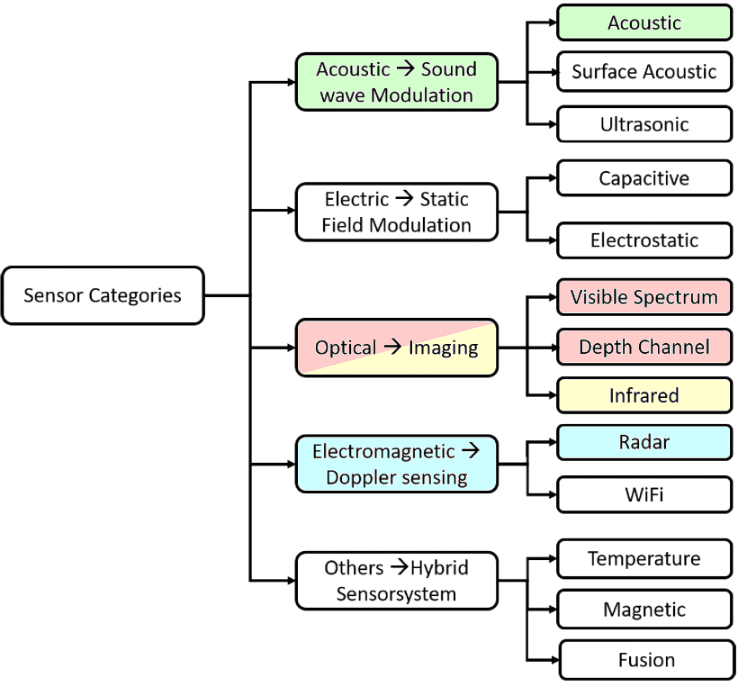
\includegraphics[width=0.7\textwidth]{fig/2/sensor-categories.png}
    \caption{
        Sensor categorization model by Fu et al. \cite{sensing-survey}.
        Data modalities present in the data collection system of this thesis are highlighted in different colours.
    }
    \label{fig:sensor-categories}
\end{figure}

The sensors are mounted on a single steel plate,
giving them an uniform perspective to the target.
The mounting bracket can be attached to a standard camera tri-pod.
The system is very portable as the sensors can be connected via USB to a computer,
and only two of the devices require an external power source:
USB cannot deliver enough power for the radar device, and the microphone requires a 12-volt input voltage.

The mounting bracket and the positions of the sensors on it are illustrated in Figure \ref{fig:sensor-array}.
The mounting bracket is drawn in white.
The blue outline represents the components of the radar device,
yellow outline represents the infrared camera,
red outline represents the RGB-D camera,
and the green outline represents the microphone.
The deeper-coloured circles represent the screw holes the sensors were mounted on.
The white circle represents the tri-pod attachment point.

\begin{figure}[H]
    \centering
    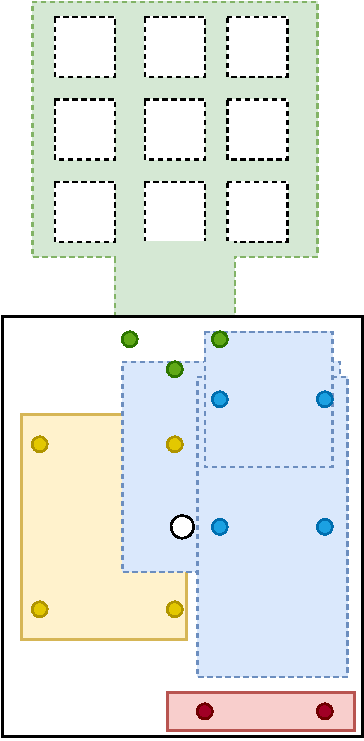
\includegraphics{fig/3/sensor-array.pdf}
    \caption{The sensor array illustrated, not in scale.}
    \label{fig:sensor-array}
\end{figure}

With the sensors chosen,
before a data collection campaign can ensue,
software needs to be written to interface with the sensors and to record the data produced by them.
The contribution of this thesis in the data collection project is to develop this software.

The following sections (\ref{sec:2-radar}--\ref{sec:2-mic}) will discuss the operating characteristics, connection interfaces,
and recorded data modalities of the included sensors.
Finally, Section \ref{sec:2-requirements} will discuss the requirements
and evaluation criteria for the data collection software developed for this thesis.

\section{Radar}
\label{sec:2-radar}
The radar used in the assembly is a Texas Instruments IWR6843ISK mmWave radar evaluation board.
It is capable of outputting various continuous radar signals.
It operates on 60--64 GHz frequency and has a maximum of 120-degree horizontal \gls{fov} and 30-degree vertical \gls{fov}.
It has a monostatic radar with distinct transmitting and receiving antennas mounted side-by-side.
The receiving antenna is a uniform linear array that consists of four antennas with 1/2-wavelength separation.
The transmitting antenna consists of three antennas, also separated by 1/2-wavelength.
The transmitting antenna is non-linear with the middle antenna slightly raised.
The antennas are illustrated in figure \ref{fig:antennas}.

\begin{figure}[H]
    \centering
    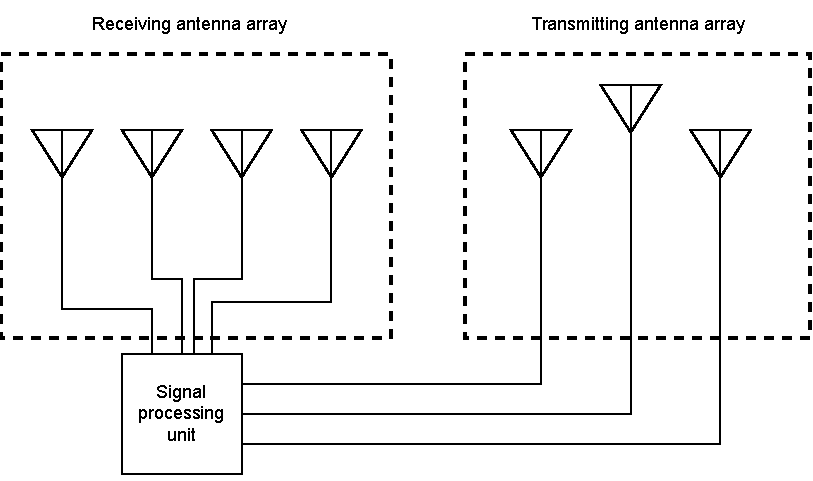
\includegraphics[width=0.8\textwidth]{fig/3/antennas.pdf}
    \caption{Antenna arrays illustrated. More detailed documentation is available in the device user guide \cite{ti-iwr-user-guide}.}
    \label{fig:antennas}
\end{figure}

By using all of the antennas,
the location of the target can be detected in all three dimensions.
The antennas can be toggled on and off via a special configuration file.
The same configuration file can be used to define nearly arbitrary signal formats. \cite{mmwave-sdk-user-guide}

The IRW6843ISK is capable of processing the radar samples into radar frames on-board,
but but depending on the operating parameters,
its performance is limited to around 1--4 frames per second.
To get more performance out of the device,
the DCA1000EVM is used to interface with the IWR6843ISK to record the raw samples without processing them on-board.
The processing is instead done separately by external software to form the radar frames.

The DCA1000EVM outputs the radar samples in a rather complicated format,
that is documented in detail in the user guide for the device.
The frames output by the device depend on its configured operating mode.
In this system, the device is configured in such a way that the frames consist of a 4-byte sequence number,
6-byte length field and a 48--1462-byte payload. \cite{dca1000-user-guide}.

\begin{figure}[H]
    \centering
    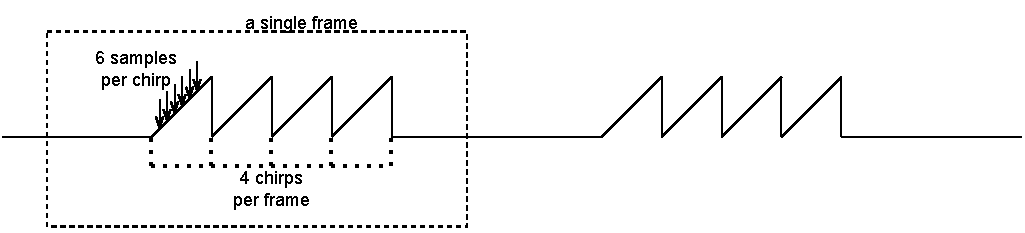
\includegraphics[width=0.9\textwidth]{fig/2/2-radar-sampling.pdf}
    \caption{Illustration of samples, chirps, and frames. With 2 receiving antennas,
    the equation \ref{eq:bytes-per-frame} would give $N = 4\cdot6\cdot4\cdot2 = 192$ bytes per frame.
    In a practical situation, the numbers would, of course, be much higher.}
    \label{fig:2-radar-signal-sampling}
\end{figure}

The data field of the frames consist of 2-byte complex samples,
that can be arranged to 4-byte I/Q samples \cite{dca1000-raw-data-capture},
i.e. four bytes of data are output for each sample.
The number of samples in a single radar frame can therefore be calculated as give nby equation \ref{eq:bytes-per-frame}.

\begin{equation}
\label{eq:bytes-per-frame}
    N = 4 \cdot S \cdot C \cdot K,
\end{equation}

where $N$ is the number of samples per frame,
$S$ is the number of samples per chirp,
$C$ is the number of chirps per frame,
and $K$ is the number of active receivers.
Figure \ref{fig:2-radar-signal-sampling} illustrates the formula.

As the frames output by the DCA1000EVM do not correspond exactly to the $N$-byte radar frames,
the data segments should simply be concatenated in the order indicated by the sequence number until a full frame can be stored or processed.
The developed data collection software saves the data segments on disk as-is,
and the exact format of the data segments is presented in more detail in Section \ref{sec:radar-file}.

The radar sensor has proven to be effective in \gls{har}.
Unlike optical and acoustic sensors,
radar is insensitive to environmental factors such as weather, lightning and acoustic noise.
It is also capable of sensing through most (non-conductive) walls,
making it less prone to occlusion.
Using \gls{mmWave} frequencies, radar is capable of detecting movements even in the sub-millimeter range.

After processing, multiple various information can can be extracted from the data:
\begin{itemize}
    \item range
    \item azimuth and altitude angle
    \item Doppler-spectrum (velocity as a function of range)
    \item radar cross-section
\end{itemize}
From \gls{har} perspective, the first three items of the list are the most interesting,
especially the doppler-spectrum (time-frequency spectrogram) \cite{sensing-survey}.

The radar can effectively detect various activities based on the Doppler-spectrum
\cite{bumblebee-micro-doppler-har, seifert19, liu12, kim16}.
Additionally it can very effectively measure the location of a target,
which can be used as additional information for other sensors.
As a downside, radar devices are very expensive and power-consuming.
This can limit its usefulness in low-power or low-budget applications.

\section{Optical}
The optical sensors consist of conventional visible spectrum imaging (RGB video),
depth imaging, and infrared imaging.
The system in this thesis includes sensors that can record all these modalities.
The Intel RealSense D435i is capable of both visual spectrum and depth imaging,
while the Panasonic Grid-EYE records the \gls{ir} spectrum.

Visible spectrum video is one of the best studied areas in computer vision and \gls{har}.
The primary approach to \gls{har} from RGB video is using convolutional neural networks.
Models such as AlexNet \cite{alexnet}, and C3D have proven to be effective,
the latter reaching as high as 90 \% accuracy in detecting human actions \cite{c3d}. 

Using a stereo camera, depth information can be extracted.
This allows for much simpler segmentation and pose estimation
compared to RGB video. \cite{sensing-survey}
Combining the RGB and depth channels,
detection accuracies as high as 98 \% have been recorded on some data sets \cite{cippitelli16}.

RGB video based segmentation and \gls{har} in general can be problematic in some scenarios.
If the image has poor contrast, proper segmentation may not be possible.
In addition to unfortunate colors,
this may be caused by bad lightning conditions, i.e. under- or overexposure or extreme fog.
Visible spectrum imaging also raises some privacy concerns in certain environments.

Thermal cameras are capable of detecting the heat radiation emitted from warm objects.
This makes them capable of detecting human motion from the background regardless of the lightning conditions \cite{han05}.
Additionally, very low resolution (from 8x8 px to 16x16 px) \gls{ir} sensors
have been demonstrated to be capable of detecting human actions \cite{10.1145/2632048.2636084}.
With a frame rate of 10 fps, detection accuracy of 85 \% and above has been reached depending on the action \cite{sensing-survey, tao18}.
Although the detection accuracy is not as good as with the RGB-D camera,
the possibility of operating in any lightning conditions and with high respect to privacy
make the \gls{ir} camera a viable choice.

\subsection{RGB and Depth video}
The RGB and Depth modalities are provided by an Intel RealSense D435i RGB-D camera.
The D435i model uses a stereo camera aided by an infrared dot matrix to measure depth,
making it similar in operating principle to the popular Microsoft Kinect.

The depth camera has a 87-degree horizontal \gls{fov} and a 58-degree vertical \gls{fov}.
It can record up to 90 frames per second with up to 1280x720 pixel resolution.
The ideal operating range is 0.3--3.0 meters and the depth measurement error is <2\% at 2 meters.
The RGB camera has a 69-degree horizontal \gls{fov} and a 42-degree vertical \gls{fov}.
It can record at up to 1920x1080 resolution and up to 30 frames per second. \cite{realsense-datasheet}

Intel provides a library that can be used to interface with the camera programmatically.
The library can be used natively from C++,
and wrappers are provided for multiple languages and toolkits,
perhaps most importantly Python, Matlab, and ROS (1 and 2).
\cite{librealsense2}
The Python wrapper was used in the data collection software.
It provides methods for getting the RGB-values, depth-values and time stamps of each frame \cite{librealsense2-python-docs}.
 
\subsection{Infrared}
The \gls{ir} camera used in the assembly is the Panasonic GRID-EYE (part no. AMG8834).
It is an infrared camera with a resolution of 8-by-8 pixels.
It has both vertical and horizontal \gls{fov} of 60 degrees,
making each pixel 6-by-6 degrees.
It can operate in temperatures of 0--\SI{80}{\celsius},
and measure temperature with a resolution of \SI{0.5}{\celsius},
while the absolute temperature accuracy is 2.5--\SI{3.0}{\celsius}.
According to the manufacturer,
it can produce data at the rate of either 1 or 10 frames per second. \cite{grid-eye-manual}
While developing the data collection software,
it was measured that the actual frame rate was approximately 8.62 frames per second, though.

The evaluation kit outputs data in 135-byte segments,
where the first 3 bytes are header bytes, followed by 130 bytes of data, and 2 bytes of tail (padding).
The first two bytes of the data represent the temperature 
of the internal thermistor of the device (ambient temperature)
and the following 128 bytes represent the \gls{ir} camera matrix packed in row-major order.
Temperatures are represented as multiples of four with little-endian two-byte integers. \cite{grid-eye-protocol}
The real temperature is therefore the unpacked number divided by four.

\section{Audio}
\label{sec:2-mic}
The microphone used in the assembly is a MiniDSP UMA-16,
which is a 4-by-4 uniform rectangular array of microphones.
It is capable of sampling at up to 48 kHz.
Other possible sampling rates are 8, 11.025, 12, 16, 32, and 44.1 kHz.
The microphone uses 24-bit quantization.

The microphone connects to the computer via USB,
and can be interfaced with like any other microphone.
Multiple convenience libraries exist for interfacing with microphones via code.
Examples include SoundDevice (Python)\cite{sounddevice-docs},
Simple DirectMedia Layer 2.0 (C, C\texttt{++}, C\#, Python)\cite{SDL2}, PortAudio (C, C\texttt{++})\cite{portaudio}.

\section{Data recording software requirements}
\label{sec:2-requirements}

To produce a high-quality data set,
some requirements are also set for the software that ties the sensors together.
In addition to giving guidelines for developing the data collection software,
having defined requirements also allows evaluating the quality of the product.

As stated earlier in this chapter,
the sensor array could be improved by including some different sensors.
Therefore, the software must be extensible.
The latency between data generation and application of time stamps must also be minimized,
which calls for parallelism.
In addition to software design choices, there are some requirements for the data it produces.
The data shall:
\begin{itemize}
    \item be time-synchronized,
    \item be labelled,
    \item be well-structured, and
    \item include sufficient metadata.
\end{itemize}

Time synchronization, in the case of the data set,
means that the beginning of the data in each recorded modality
corresponds to the same point in time.
In other words, given a common starting time $T_{s}$,
the first data point should correspond to $T_{s}$ in each recorded modality.
In addition, the recorded data for any modality shall not end before a common ending time $T_{e}$.
Given a known sampling rate $N_{s}$,
satisfying this requirement allows easily mapping any moment in time ($t$) to a sample number ($n$) (equation \ref{eq:time-to-sample}).

\begin{equation}
    \label{eq:time-to-sample}
    n = \mathrm{round}(N_{s} t)
\end{equation}

For the data to be useful in supervised learning,
the current activity at any given time must be included in the data set;
the data must be labelled.
Labelling can be done in various ways.

The most accurate labelling method is manual labelling:
someone goes over the data and applies appropriate labels to each activity.
Although this results in superior accuracy,
it is very laborious and therefore not very desirable.

The activities could also be sourced from some sensors and algorithms that are 
already capable of recognising activities with a high accuracy.
As previously stated, there are numerous algorithms that can recognize activities from RGB-D video.
The RGB-D video provided by the sensor array could therefore be used to map labels for the activities on the time domain.
Using equation \ref{eq:time-to-sample}, the labels could then be generalized for the whole data set.

In addition to time synchronization and labels,
the data must be structured in such a way that the data produced by each sensor in a single recording
can be mapped to one another and the corresponding metadata and labels.
It would additionally be beneficial to be able to pick and choose the sensors that are processed.
The simplest way to achieve this is to produce one file per sensor and store them in a common directory.
Another way would be to pack the data from different sensors into a single file,
but this would be rather complicated especially because the recorded data is heterogenous in length.

\chapter{System implementation}
\label{ch:3-system}
The system was implemented completely using Python (3.10),
which is one of the most widely known programming languages \cite{developer-survey}.
Multiple libraries exist for Python for implementing a wide variety of tasks.
Using high-level libraries is expected to save development time and the popularity of Python
is expected to make the source-code easily approachable for future programmers.

To minimize the latency in reading the data from the sensors,
the system was designed to use parallelism.
The system implements a producer-consumer pattern,
using the Python build-in Multiprocessing library.

The Multiprocessing library is the best of the python built-in parallelism libraries for the task at hand.
The program is synchronous, hence Asyncio is perhaps a too complex solution \cite{python-asyncio}.
While the Threading library would otherwise be a good solution,
it is not truly concurrent as the Python \gls{gil} locks its thread model to a single process \cite{python-threading}.
Multiprocessing, instead, implements process-level parallelism and is capable of achieving "true" concurrency \cite{python-multiprocessing}.

The structure of the program is presented in Figrure \ref{fig:3-block-diagram} as a block diagram.
The program consists of a Main block and five sub-blocks:
\begin{itemize}
    \item Recorder,
    \item Radar module,
    \item RGB-D module,
    \item Infrared module, and
    \item Microphone module.
\end{itemize}

The aforementioned producer-consumer pattern is implemented with all the different blocks being created as parallel processes.
The Radar, Microphone, Infrared and RGB-D modules fetch data from the sensors, making them producers.
The producers output data to queues which are then read by the Recorder block,
hence the Recorder is a consumer.
The main block is neither a producer or a consumer; rather it is responsible for allocating resources for the sub-blocks,
spawning the sub-block processes (subprocesses), controlling them, providing a user interface and writing the metadata file.

\begin{figure}[h]
    \centering
    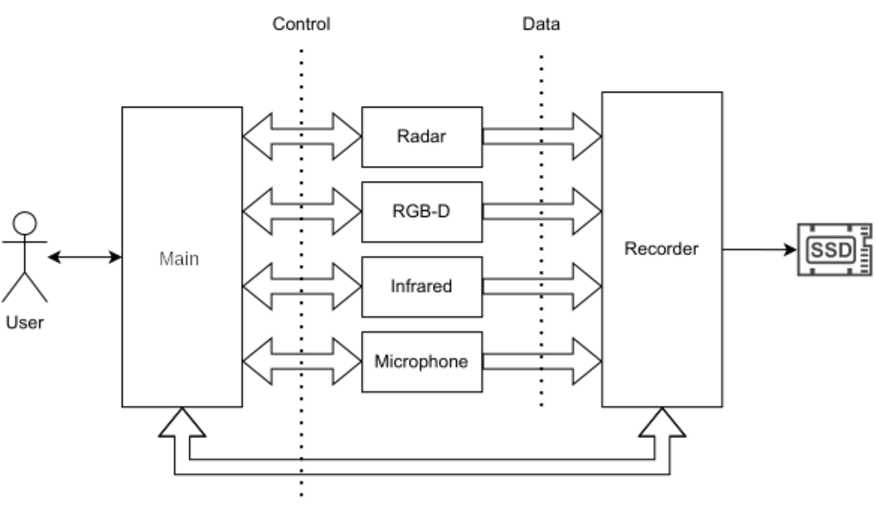
\includegraphics[width=.8\textwidth]{fig/3/block_diagram.pdf}
    \caption{Block diagram of the system.}
    \label{fig:3-block-diagram}
\end{figure}

Inter-process communication is done via \gls{fifo} queues.
Each subprocess is connected to the main process via a single queue.
These queues are colloquially called signaling queues.
In addition, the producers are connected to the Recorder via queues,
one queue per producer. These queues are called the data queues.
The main process creates all these queues and passes them to appropriate subprocesses.

Queues are presented in Figure \ref{fig:3-block-diagram} as single- or double-headed arrows.
A double-headed arrow means that the queue can be written to and read from in both ends,
and single-headed arrow means that data can be read from the pointy end and written from the other.
The signaling queues are read from and written to from both ends,
whereas the data queues are only written to by the producers and read from by the consumer.

While using multiple queues introduces some complexity to the system,
it prevents having to deal with race-conditions.
Another option would have been to use only a single Data queue
and to lock it for writing via mutexes in each of the producers.
The locking operation can block if the mutex is locked from somewhere else,
which could add latency to the data reading operations,
making the multiple queues -approach a better solution.

The control queues are used by the Main process to advance the subprocesses to their next phase.
The subprocesses write to the control queues to indicate their state.
Three kinds of control messages are defined: START, STARTED, and STOP.
The control messages are simply Python String objects with defined content and meaning.
The control messages are documented in Table \ref{tab:control-messages}.

\begin{table}[H]
    \centering
    \begin{tabular}{l l l}
        \toprule
        \textbf{Message} & \textbf{Sender} & \textbf{Meaning} \\
        \midrule
        START & Main & Recipient should start its primary function \\
        STARTED & Producers & Sender has initialized and entered its primary function \\
        STOP & Main & Recipient process should exit \\
        \bottomrule
    \end{tabular}
    \caption{Control messages in the program}
    \label{tab:control-messages}
\end{table}

The flow of the processes consists of three phases: initialization, primary function, and cleanup.
The Main process and the data producers enter the primary function autonomously after the initialization phase is over.
The data producers write the STARTED message to the control queue after this transition.
The Recorder process instead waits for the START message before transitioning from initialization to primary function.
None of the subprocesses enters the cleanup phase autonomously.
They all wait for the Main process to write the STOP message to the control queue before transitioning.
The phases of the subprocesses are discussed in more detail in Sections \ref{sec:3-recorder}--\ref{sec:3-mic}.

The initialization phase of the Main process consists of parsing command line arguments,
spawning the subprocesses, and waiting for the STARTED messages.
After receiving the STARTED message from aech data producer,
the Main process sends the START message to the Recorder process and enters its primary function, which is a user interface loop.

The user interface is a simple interactive command line interface that can be used for semi-automatic data labelling and stopping the program.
A file containing activity labels is provided via the command line arguments to the program.
The program reads activities separated by a newline character into a list,
and each time the user hits the Enter key,
the time elapsed since sending the START message is recorded.
The activity and timestamp are then written into a file and the list iterator is advanced.
When either the list ends, the current activity label is "STOP", or the user writes the "q" character and then presses Enter,
the primary function of the Main process ends, and the user interface loop is exitted.

After ending the primary function,
it records the stopping time and sends the STOP signal to the data producers.
After sending the STOP signal, the Main process waits for the data producer processes to exit.
Then it sends the STOP signal and the current time to the Recorder process and waits until the process exits.
After all the subprocesses have exitted, the Main process writes the metadata file and exits,
ending the program.
The flow of the main process is represented as a flowchart in Figure \ref{fig:3-main-flowchart}.

\begin{figure}[H]
    \centering
    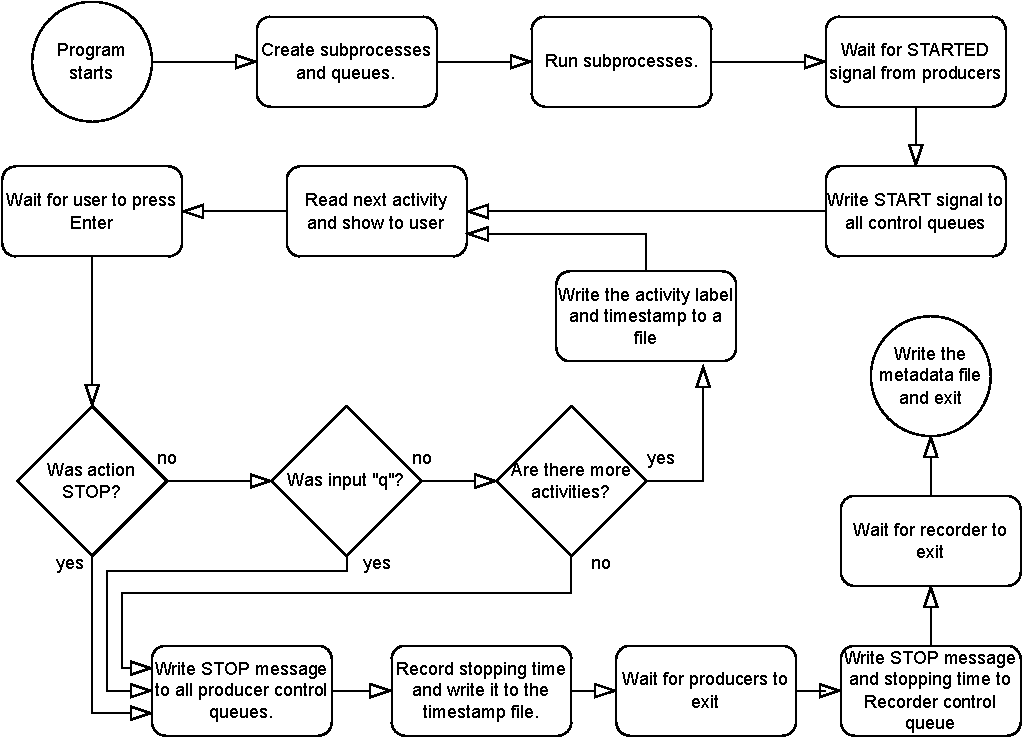
\includegraphics[width=0.9\textwidth]{fig/3/main-flowchart.pdf}
    \caption{Flow of the main process}
    \label{fig:3-main-flowchart}
\end{figure}

The following Sections (\ref{sec:3-recorder}--\ref{sec:3-mic}) will document the implementation of the subprocesses.
For the data producers, communication with the sensors will be documented, and for the Recorder,
the time-domain synchronization mechanism will be documented.
The three phases of operation will be described similar to the former description of the Main process.
Section \ref{sec:3-usage} will briefly cover usage of the software.

\section{Recorder block}
\label{sec:3-recorder}
The Recorder module is the only consumer in the program.
It takes the data produced by the producers and writes it into a file.
It is also responsible for time-domain synchronization of the different data streams.

The initialization phase of the Recorder block consists of opening file handles for the output files and initializing some counters.
In the beginning of the second phase, i.e. after receiving the START message,
the Radar block finds the common starting point for each data producer and synchronizes the data streams to the common starting point.
After the data streams are synchronized, the Recorder enters a loop in which it simply reads the data from each data queue and writes it onto a disk.

Time synchronization is achieved in the Recorder block by observing the time stamps that the producers add to the packets they write in data queues.
Each packet is a dict object that contains a segment of data and the time stamp when the data segment was recorded.

By the time the START message is received from the control queue,
all the data producers have started producing data and have written their first message to the data queues.
After the START message, the Main process also writes the current time to the control queue of the Radar block.
The common starting point is found by comparing the time stamps in the data queues to the starting time provided by the Radar block.
The data in each data queue is simply discarded until the timestamp is within half-a-frame from the starting time.
After the appropriate amount of data has been discarded from each queue,
the data streams are synchronized and the Recorder starts writing the data into files.
The data starting point synchronization procedure is presented in pseudocode in Listing \ref{lst:synchronization}.
The half-a-frame accuracy is omitted from the listing for brevity.

\begin{lstlisting}[language=Python, caption={Data synchronization pseudocode}\label{lst:synchronization}]
while control_queue.pop() != "START":
    pass
start_time = control_queue.pop()

for queue in data_queues:
    message = queue.pop()
    timestamp = message["timestamp"]
    data = message["data"]
    
    while (timestamp < start_time):
        message = queue.pop()
        timestamp = message["timestamp"]
        data = message["data"]
\end{lstlisting}

Finally, when the user stops the system, the Main process sends the STOP message to the Recorder control queue,
and in succession, the stopping time .
By this time, the data producers have already exitted and no more data will be written to the output queues.
The Recorder then enters the last phase of operation,
which is the stream end synchronization.

The stopping time is recorded before the STOP signal is sent to the data producers.
Knowing this, finding the common ending point is trivial,
and the algorithm presented in Listing \ref{lst:synchronization} can be modified for the purpose.
Instead of the starting time, the time stamps are compared to the ending time,
and instead of discarding the data, it is written into a file.
The modified algorithm is presented in Listing \ref{lst:end-synchronization}.

\begin{lstlisting}[language=Python, caption={Data synchronization pseudocode}\label{lst:end-synchronization}]
while (control_queue.empty() or control_queue.pop() != "STOP"):
    for queue in data_queues:
        message = queue.pop()
        data = message["data"]
        # write data to file
        
end_time = control_queue.pop()

for queue in data_queues:
    message = queue.pop()
    timestamp = message["timestamp"]
    data = message["data"]
    
    while (timestamp < end_time):
        message = queue.pop()
        timestamp = message["timestamp"]
        data = message["data"]
        # write data to file
\end{lstlisting}

After the end synchronization procedure is finished,
the Recorder will flush the data queues discarding all remaining data,
and close the file handles.
After freeing the resources and flushing the queues, the process will exit.

\section{Radar block}
\label{sec:3-radar}
The radar module actually consists of two devices: the Texas Instruments IWR6834ISK and the DCA1000EVM Radar Data capture card.
In this section, the former is referred to as the "radar device" and the latter as the "capture card".
The radar device connects to the computer via USB and implements a simple serial interface.
The capture card uses Internet Protocol version 4 to connect to the computer and transfers data over the User Datagram Protocol.

In the Radar block, the Pyserial third-party library is used to connect to the serial interface.
The Pyserial library implements an easy-to-use high-level serial port \gls{api}. \cite{python-serial}
The serial port was configured to use a baud rate of 115200 bps and no parity.

For reading data from the capture card, the built-in Socket library is used.
The Socket library implements the Berkeley Socket interface.
By default, the capture card is listening at address \texttt{192.168.33.180:4096} and sends data to address \texttt{192.168.33.30:4098}.
The addresses could be configured differently, but it was deemed easier to just configure an extra \gls{ipv4} address to the host computer. \cite{dca1000-user-guide}

In the initialization phase, the Radar block configures the radar device and the capture card.
Configuring the radar device is done by writing a special configuration file to the serial interface.
The exact format of the configuration file is documented in the Texas Instruments mmWave SDK user guide \cite{mmwave-sdk-user-guide}.
The configuration file used during the testing and development of this system is included as Appendix \ref{app:config}.

The capture card is configured by transmitting special configuration packets to the address it is listening to.
The packets consist of a header (\texttt{0x055A}), a two-byte unsigned integer length field, command identifier, body, and a footer (\texttt{0xEEAA}).
The commands are listed in the DCA1000EVM user guide \cite{dca1000-user-guide} and the details of the command bodies are documented in 
DCA1000EVM CLI Software Developer guide, which is included in the Texas Instruments mmWave studio collection of tools \cite{mmwave-studio}.
For the sake of availability, the commands and their bodies are also documented in Appendix \ref{app:dca1000evm-commands}.
While most settings are left to default values, the LVDS mode is changed to 2lane and Data format mode is changed to 16-bit.
This is done via the CONFIG\_FPGA\_GEN\_CMD\_CODE command (Appendix \ref{app:dca1000evm-commands}, Section \ref{app:sec:config-fpga}).

After configuration is done, the devices must also be started.
The radar device can be started by writing "\texttt{sensorStart\textbackslash n}" to the serial interface.
The capture card is started by sending the RECORD\_START\_CMD\_CODE (Appendix \ref{app:dca1000evm-commands}, Section \ref{app:sec:start-record}).
The capture card should then respond with status 0, indicating that the recording has been successfully started,
thus concluding the initialization phase.

After starting the radar device and the capture card,
the Radar module writes the STARTED message to the control queue and begins its primary function phase.
In the primary function,
the Radar module listens to the socket \texttt{192.168.33.30:4098} and reads data from it whenever available.

The Radar process can read the number of samples per frame from the radar configuration file.
With this information, it is possible to organize the received data into frames and write them into the data queue frame-by-frame.
The inter-frame time is also known from the configuration file.
The radar device or the capture card do not add any timing information to the outputted data.
The Radar process therefore records the current time when the first byte of the first frame is received, i.e. the starting time.
The starting time is then used to calculate time stamps for the frames.
For each received frame, a counter is incremented. The time offset of the frame is calculated from the counter and the inter-frame time and added to the starting time
to form the time stamp for the frame.

The process simply reads data from the socket to a buffer until the buffer contains a single frame.
When enough data is in the buffer, a dict-object containing the data of the frame and a time stamp for the frame is written into the data queue.
The frame is then deleted from the beginning of the buffer and the loop is continued until the STOP message is received.
The flow of the Radar module is represented as a flow chart in Figure \ref{fig:3-radar-flowchart}.

\begin{figure}[H]
    \centering
    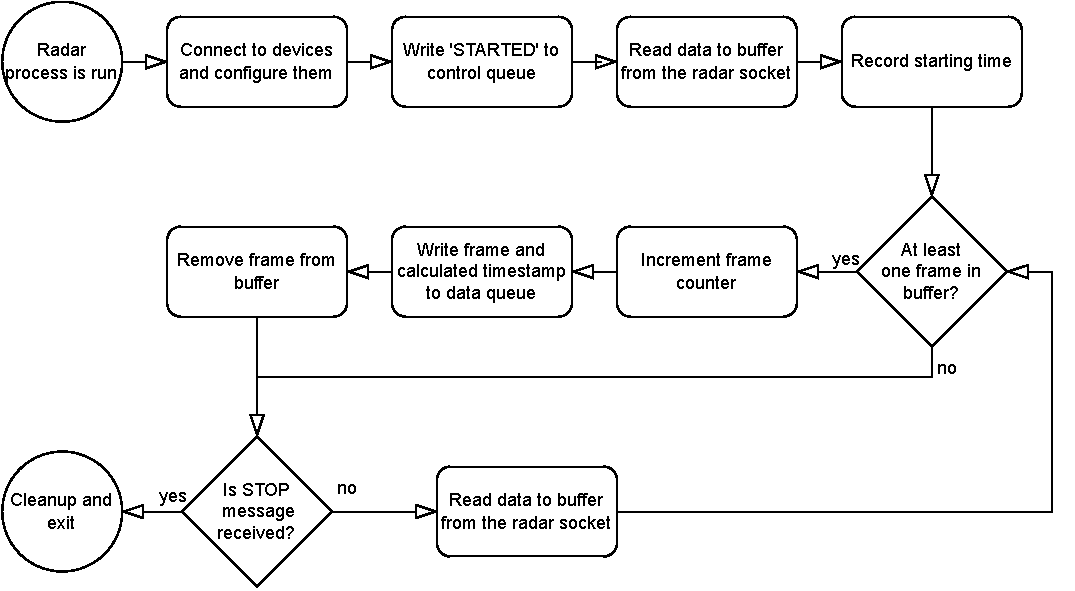
\includegraphics[width=\textwidth]{fig/3/radar-flowchart.pdf}
    \caption{Flow of the Radar module}
    \label{fig:3-radar-flowchart}
\end{figure}

After the STOP message is received,
all the sockets and serial connections are closed.
Additionally, the remaining data from the buffer is discarded and the data queue is closed from being written to.
Thus, the clean up is concluded and the Radar process exits.

\section{RGB-D block}
\label{sec:3-rgb-d}
Intel provides the Librealsense library for working with the camera with multiple programming languages.
For this implementation, the Pyrealsense2 library was used, which implements Python bindings for the Librealsense library. \cite{librealsense2}
The Librealsense provides a high-level \gls{api} for configuring the device and reading data from it.
Configuring is done via a \texttt{Config} object and reading data is done via a \texttt{Pipeline} object. \cite{librealsense2-python-docs}

In the initialization phase of the RGB-D process, the \texttt{Config} and \texttt{Pipeline} objects are created.
The used data streams must be explicitly enabled via the \texttt{Config} object.
The depth and color streams are enabled.
The functions that enable the streams also configure the frame rate, resolution, and number format for the data.
In this implementation, the resolutions and frame rates are read from a configuration file provided by the user.
The colored stream is configured to output data in the RGB8 format, where each pixel is represented by three bytes.
The bytes are one-byte unsigned integers. The first byte is the red value, second byte is the green value and third byte is the blue value.
The depth stream is configured to output data as 2-byte floating point numbers,
where each pixel, or a 2-byte floating point number, represents the distance from the camera in the direction of the pixel.

After configuring the data streams, the \texttt{Pipeline} object is used to start the sensor.
After the sensor has been started, the process writes the STARTED message to the control queue and enters its primary function.

In the primary function, the process reads frames from the \texttt{Pipeline} object using a member function of the Pipeline object that blocks until a frame is available.
The function call returns a \texttt{composite\_frame} object that contains the stream data, a time stamp, and some other less interesting metadata.
The RGB-D process reads the color stream data and the depth stream data into arrays and stores them in a \texttt{dict} object along the time stamp for the frame,
which is also read from the \texttt{composite\_frame}.
The \texttt{dict} object is then written into the data queue and the process is repeated until the STOP message is received from the control queue.

When the STOP message is received,
the RGB-D process transitions into its cleanup phase.
In the cleanup phase, the process simply exits,
which calls the destructors of the Pyrealsense2 objects,
which in turn stop the sensors and free their allocated resources.
Figure \ref{fig:3-rgbd-flowchart} illustrates the flow of the RGB-D process.

\begin{figure}
    \centering
    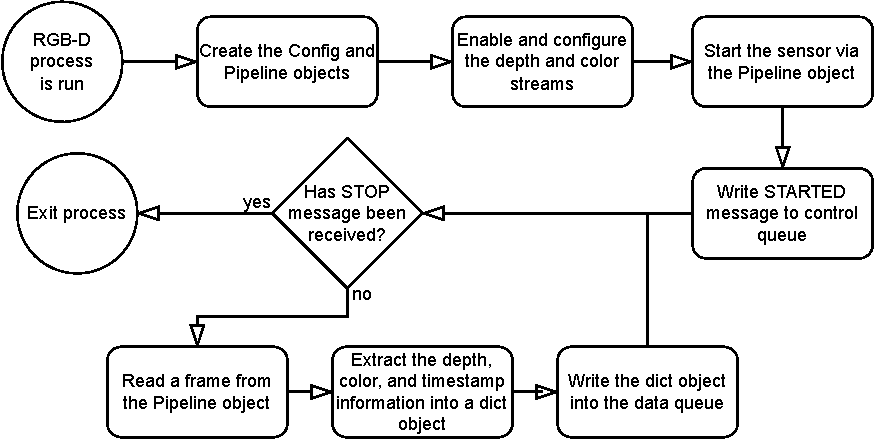
\includegraphics{fig/3/rgbd-flowchart.pdf}
    \caption{Flow of the RGB-D process}
    \label{fig:3-rgbd-flowchart}
\end{figure}

\section{Infrared block}
\label{sec:3-ir}
Similar to the TI IWR6843ISK, the Panasonic GRID-EYE implements a simple serial interface over USB.
Pyserial was also used for connecting to the GRID-EYE.
Two kinds of packets are implemented for the GRID-EYE protocol: Sensor Data frames and Command frames.
The Command frames are used by the connecting computer to configure the device and after being started,
the device will write Sensor Data frames to the serial port.
The Command frames can be used to set the sensor into either 10 \gls{fps} for 1 \gls{fps} mode. \cite{grid-eye-protocol}
The sensor is used in the 10 \gls{fps} mode in the system, because the 1 \gls{fps} mode is only the sum of every 10 frames
and similar effect can easily be achieved by post-processing the data after recording \cite{grid-eye-manual}.

In the initialization phase, the IR process opens the serial port (9600 bps, no parity, one stop bit, 8-bit byte size).
The device requires no further configuration as it operates in the 10 \gls{fps} mode by default.
After opening the serial port, the data in the serial port is flushed,
and the STARTED message is written to the control queue,
concluding the initialization phase.

After the initialization phase, the process immediately begins the primary function.
In the primary function, the process reads data from the serial port in 135-byte chunks.
The 5th--132th (0-indexing) bytes contain the temperatures for each of the pixels as two-byte little-endian integers.
Every two bytes is a multiple of four of the temperature reading.

The Python built-in Struct library is used to unpack the raw data to numeric values.
Conveniently, two-byte floating point numbers can accurately represent integer multiples of $0.25$.
Using this knowledge, the unpacked numbers are divided by four and repacked as two-byte floating point numbers.
The repacked floating point numbers are then stored in a \texttt{dict} object with a time stamp that is sourced 
from the computer clock using the \texttt{perf\_counter} function from the Python built-in Time library.
The process is then repeated until the STOP message is received from the control queue.

After receiving the STOP signal, the clean-up phase begins.
In the clean up, the process simply exits,
which frees the serial port file handle.
No other resources were allocated in the process.
The flow of the system is illustrated in Figure \ref{fig:3-ir-flowchart}.

\begin{figure}
    \centering
    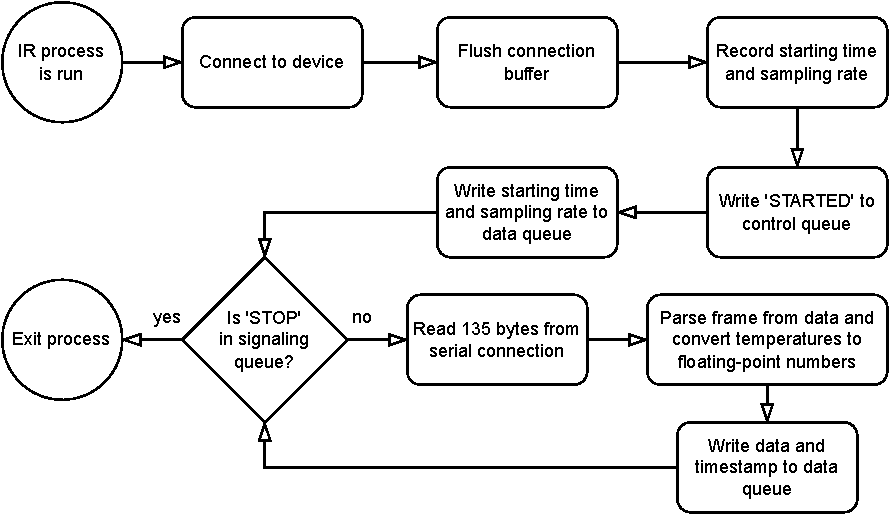
\includegraphics[width=\textwidth]{fig/3/ir-flowchart.pdf}
    \caption{Flow of the IR process}
    \label{fig:3-ir-flowchart}
\end{figure}

\section{Microphone block}
\label{sec:3-mic}
Unlike the other devices, the data produced by the microphone cannot be organized into frames.
It produces a continuous stream of data on all 16 channels at a configurable sampling rate and bit depth.
The SoundDevice library is used for interfacing with the device \cite{sounddevice-docs}.
It provides Python bindings for the PortAudio library,
which, among other features, has the ability to pick a sound device,
configure it to a wished sampling rate and bit depth, and record audio from it \cite{portaudio}.

Picking a device is done via the \texttt{query\_devices} function,
which returns information about available devices.
It accepts two arguments.
The first argument is a numeric device ID or the name of the device as a string.
If the first argument is given, only the information of one device is returned.
The second parameter can be used to list only input or output devices. \cite{sounddevice-docs}.

The SoundDevice library implements an \gls{api}, where \texttt{Stream} objects are created and attached to audio devices.
The \texttt{Stream} objects can then write to and read from devices.
A callback function may be passed to the constructor of the \texttt{Stream} object,
which is periodically called automatically by the PortAudio library.
The callback function handles writing data to the device and provides access to the read data. \cite{sounddevice-docs-stream}

The callback function may also be omitted,
in which case reading and writing should be done via the blocking \texttt{read} and \texttt{write} functions.
Using the callback function is the preferred way of using the interface,
as the callback function automatically has a high processing priority.
To achieve robust audio with minimal latency, 
the callback function should not call functions with long or unpredictable execution times. \cite{sounddevice-docs-stream}

After the \texttt{Stream} object has been instantiated,
the stream must also be started.
This can be done via \texttt{start} and \texttt{stop} functions.
The stream objects are also context managers and when used in the \texttt{with}-statement,
the \texttt{start} and \texttt{stop} functions are automatically called in the beginning and end of the statement, respectively. \cite{sounddevice-docs-stream}
Context managers and the \texttt{with} statement are a part of the Python programming language.

The initialization phase of the Microphone module finds the correct sound device and constructs and \texttt{InputStream} context manager,
which is a specialized \texttt{Stream} object that can only be used for input devices.
Searching the device is done via the \texttt{query\_devices} function with the first argument set to "micArray16".
The device is then set as the default device in the SoundDevice library.
Upon instantiation, the \texttt{InputStream} object will utilize the default device without further configuration.

The configuration is done in the constructor of the \texttt{InputStream} object.
The sampling rate is set to 44.1 kHz, bit depth to 32 bits and recording is done on all 16 channels of the device.
After instantiating the \texttt{InputStream} object, the STARTED signal is written to the control queue and the primary function is entered, ending the initialization phase.

The primary function is a simple busy-loop that observes the control queue.
The process runs until the STOP message is read from the control queue.
While waiting for the STOP message,
the callback function is being periodically called by the PortAudio library.
The callback function writes data from the device to the data queue along the timestamp for when the callback was called.
The timestamp is derived using the \texttt{perf\_counter} function from the built-in Time library.

\begin{figure}[H]
    \centering
    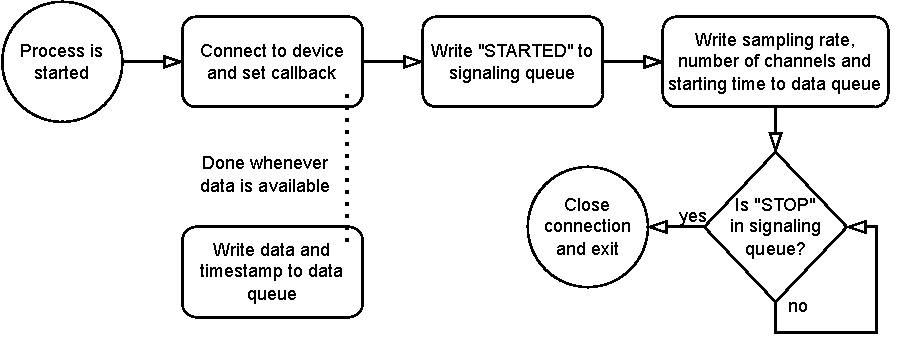
\includegraphics[width=\textwidth]{fig/3/mic-flowchart.pdf}
    \caption{Flow of the Microphone block}
    \label{fig:mic-flowchart}
\end{figure}

When the STOP message is received from the control queue,
the aforementioned busy-loop exits, ending the \texttt{with}-statement and stopping the \texttt{InputStream} instance.
The Microphone process then exits.
The logic of the Microphone process is presented as a flowchart in Figure \ref{fig:mic-flowchart}.

\section{Using the software}
\label{sec:3-usage}
The software is started via a \gls{cli} that is implemented using the Python built-in \texttt{argparse} library.
Three positional arguments must be provided for the program: \texttt{activities}, \texttt{config}, and \texttt{outdir}.
All of the arguments are file paths.

The first argument, \texttt{activities}, can be used to provide a list of activities for the software.
This can be used for semi-automatic activity labelling during the recording process.
This is useful when recording a predetermined list of activities.
The activities must be separated by newline (\texttt{\textbackslash n}) characters.
The software outputs a \gls{csv} file which contains the same list of activities,
but each activity is assigned a timestamp.
The file can also be empty, in which case no timestamps will be recorded other than the starting and stopping time.

The second argument, \texttt{config}, is a configuration file for the program.
The values present in the file are used to configure the sensors.
The file must follow the YAML data serialization language.
An example file is provided in Listing \ref{lst:config}.

\begin{lstlisting}[caption={Example configuration file}\label{lst:config}]
radar:
    config: filename
camera:
    resolution: [width, height]
    fps: integer
\end{lstlisting}

Under the key \texttt{radar}, the \texttt{filename} that is the value of \texttt{config} must refer to a configuration file for the TI IWR6843ISK radar device.
Under the key \texttt{camera}, the value of \texttt{resolution} must be a two-element list whose values are some supported resolution of the Intel RealSense 435i camera.
Similarly, the \texttt{fps} must be some supported frame rate of the camera.
The values under the key \texttt{camera} are used for both the RGB and Depth stream.
The \gls{ir} and microphone devices should preferrably be configured via the same file but due to time constraints,
they were left hardcoded.

The last argument, \texttt{outdir}, must be a directory path.
The files created by the software are written into this directory.
The output files and their exact formats are documented in Chapter \ref{ch:4-files-and-post}.


\chapter{Output file formats and post-processing}
\label{ch:4-files-and-post}
The software outputs seven files: five sensor data files, a metadata file, and a file containing time stamps and labels.
The file names and a general description of the content is documented in Table \ref{tab:3-files}.

\begin{table}[H]
    \centering
    \begin{tabular}{l l}
    \toprule
    \textbf{File name} & \textbf{Description} \\
    \midrule
    audio.wav & Microphone samples \\
    depth.raw & Depth camera record \\
    ir.raw & \gls{ir} camera record \\
    metadata.yaml & Metadata \\
    radar.raw & Radar samples \\
    rgb.raw & RGB camera record \\
    timestamps.csv & Activity labels and time stamps \\
    \bottomrule
    \end{tabular}
    \caption{Files output by the software.}
    \label{tab:3-files}
\end{table}

The sensor data files contain unprocessed (raw) data outputted by the sensors;
only the data in \texttt{ir.raw} has been repacked into a different number format.
To extract meaningful data from the files, the file formats must be understood.
Additionally, it may be beneficial to perform some post-processing for the data,
especially in the case of the \texttt{radar.raw} file.

The following sections will document the exact formats of the file
and present some relevant data processing algorithms for each data file format.

\section{Activity labels and time stamps}
The activity labels and their corresponding timestamps are stored in the \texttt{timestamps.csv} file.
As implied by the file name, the file follows the \gls{csv} format, delimited by the comma character (",", unicode U+002C).
The file contains two columns.
The first column contains time stamps and the second column contains labels.
Listing \ref{lst:labels} provides an example of the file.

\begin{lstlisting}[caption={Example \texttt{timestamps.csv} file.}\label{lst:labels}]
    0.000506,sitting
    1.689381,stand_up
    4.106970,walking
    7.184435,pick
    9.060120,walking
    12.494,STOP
\end{lstlisting}

The activities are sorted by time in an ascending order.
The time stamps tell the time elapsed since the beginning of the recording.
The frame rate (\gls{framerate}) for each sensor is recorded in the \texttt{metadata.yaml} file.
Based on the timestamps and the frame rate of each sensor, the mapping between frames and labels can be made.
The time of recording (from \gls{time-min} to \gls{time-max}) for a given frame can be calculated 
based on the frame number \gls{framenumber}
via equation \ref{eq:frame-number-to-time}.

\begin{equation}
    \label{eq:frame-number-to-time}
    \begin{cases}
        \gls{time-min} = \frac{\gls{framenumber}}{\gls{framerate}} \\
        \gls{time-max} = \frac{\gls{framenumber}+1}{\gls{framerate}}
    \end{cases}
\end{equation}

Given $\gls{time-min} \leq \gls{time} < \gls{time-max}$, where \gls{time} is the timestamp of an activity, the activity should be mapped to the frame.

\section{IR camera record}
\label{sec:ir-file}
The frames produced by the infrared block consist of 64 numbers (8x8 pixels).
The frames are stored in the \texttt{ir.raw} file.
Each pixel is represented by a half-precision (16-bit) floating point number.
The values represent the recorded temperatures in each pixel.

The pixels of each frame are stored in row-major order,
thus denoting the vector containing the recorded values as \gls{data},
the frames can be represented by equation $\ref{eq:ir-frame}$,
where \gls{frame-z} is the \gls{framenumber}:th frame, \gls{pixelrow} is the row of a pixel and \gls{pixelcol} is the column of a pixel.

\begin{equation}
    \label{eq:ir-frame}
    \forall \gls{pixelrow} \in [0, 7] \land \gls{pixelcol} \in [0, 7] \land \gls{framenumber} \in \left[ 0, \frac{|\gls{data}|}{64} \right] : \gls{frame-z}(\gls{pixelrow}, \gls{pixelcol}) = \gls{data}(64\gls{framenumber}+8\gls{pixelrow}+\gls{pixelcol})
\end{equation}

The origin of the image is in the upper left corner.
Figure \ref{fig:ir-orig} shows an example frame parsed from the file and \ref{fig:ir-rgb} shows the corresponding RGB image.
The data in frame \gls{frame-z}  may be used as-is, but the resolution of the image may be increased by interpolating.
Figures \ref{fig:ir-interp-2x} and \ref{fig:ir-interp-4x} illustrate the effects of increasing the resolution of the original image
to 16x16 and 32x32 using cubic interpolation.
A code example in Python for parsing the frames from the file is given in Appendix \ref{app:ir-parsing}.

\begin{figure}[H]
    \centering
    \begin{subfigure}[b]{0.475\textwidth}
        \centering
        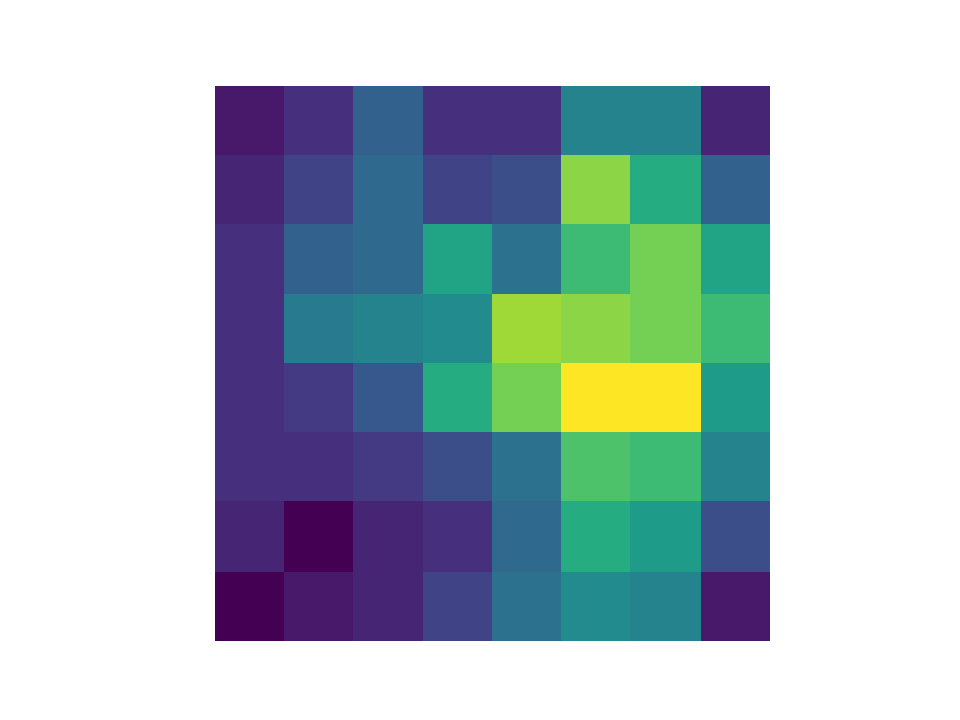
\includegraphics[width=\textwidth]{fig/4/ir-orig.pdf}
        \caption{Original 8x8 image.}
        \label{fig:ir-orig}
    \end{subfigure}
    \hfill
    \begin{subfigure}[b]{0.475\textwidth}
        \centering
        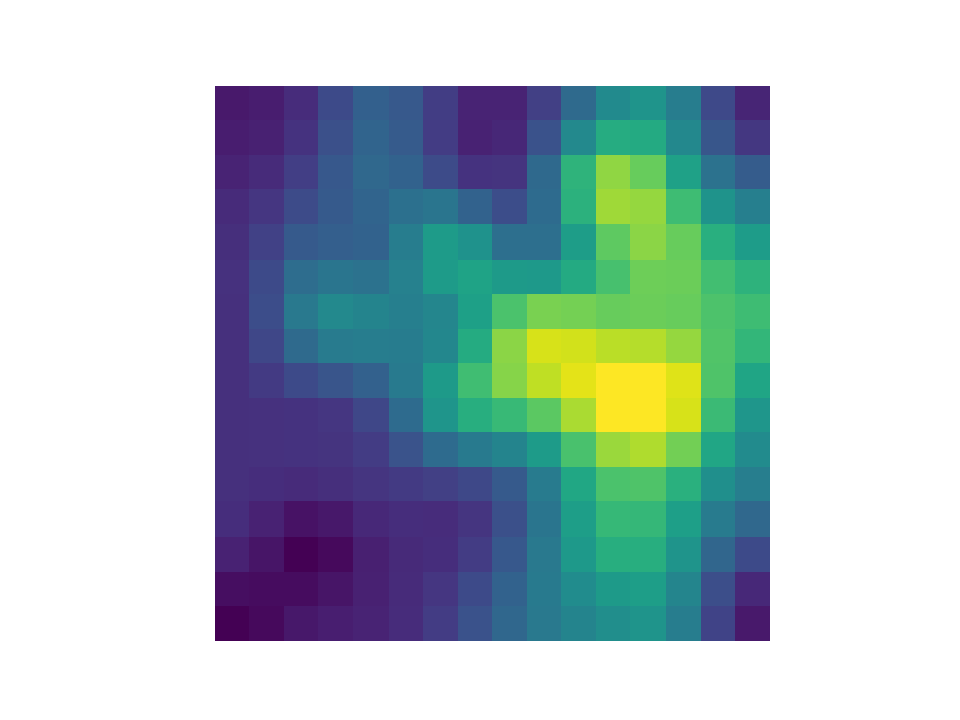
\includegraphics[width=\textwidth]{fig/4/ir16.pdf}
        \caption{Original image upscaled to 16x16 by interpolation.}
        \label{fig:ir-interp-2x}
    \end{subfigure}
    \vskip\baselineskip
    \begin{subfigure}[b]{0.475\textwidth}
        \centering
        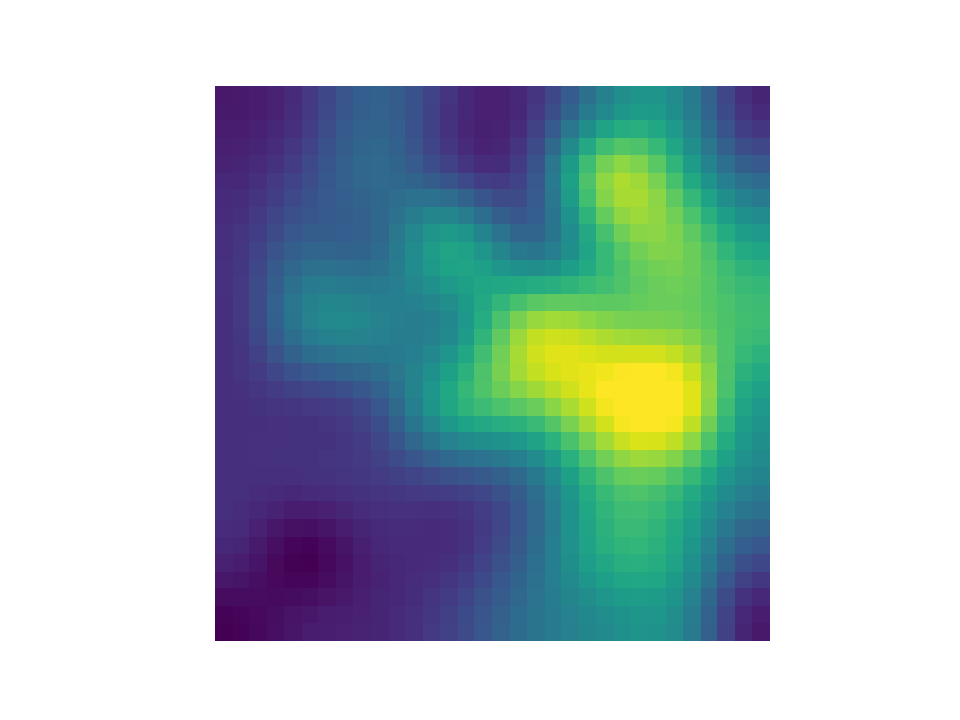
\includegraphics[width=\textwidth]{fig/4/ir32.pdf}
        \caption{Original image upscaled to 32x32 by interpolation.}
        \label{fig:ir-interp-4x}
    \end{subfigure}
    \hfill
    \begin{subfigure}[b]{0.475\textwidth}
        \centering
        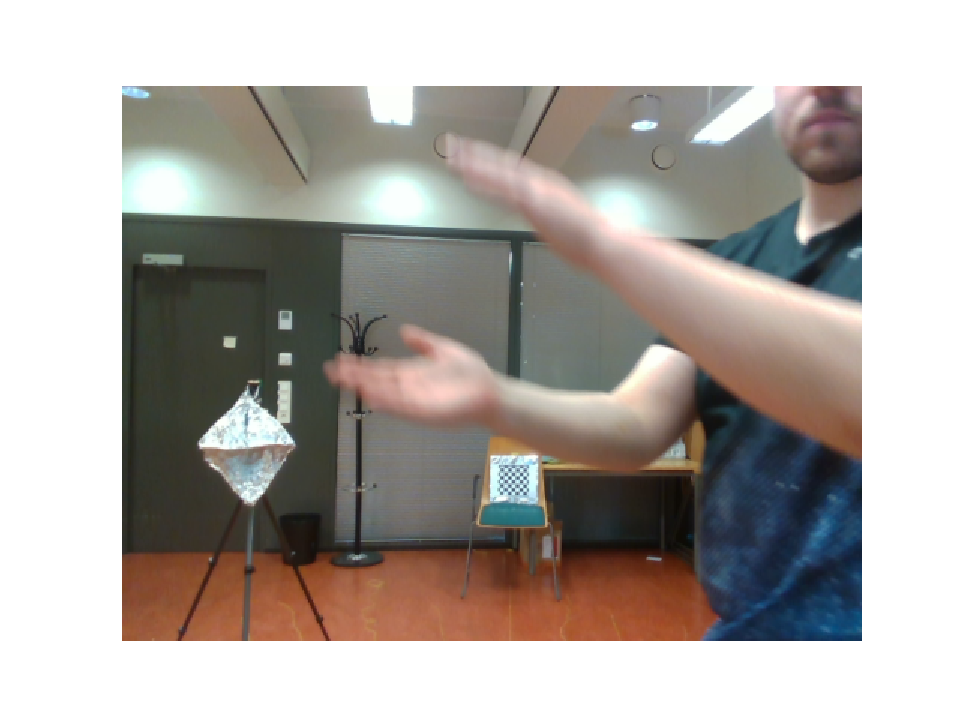
\includegraphics[width=\textwidth]{fig/4/ir-rgb.pdf}
        \caption{Corresponding RGB image.}
        \label{fig:ir-rgb}
    \end{subfigure}
    \caption{An \gls{ir} frame interpolated to different higher resolutions and the corresponding RGB frame.}
    \label{fig:ir-interpolated}
\end{figure}

\section{Radar samples}
\label{sec:radar-file}
The Texas Instruments mmWave Radar Device ADC Raw Data Capture application report defines multiple data formats for the DCA1000EVM data output format,
which is also the format the data is stored in the \texttt{radar.raw} file~\cite{dca1000-raw-data-capture}.
Combined with the TI6843ISK radar module, the data formats are limited to only one option~\cite{mmwave-sdk-user-guide}.
The data is sampled in the \gls{iq} format.
Given there are $N$ samples per chirp, $M$ chirps per frame, and $K$ active receivers,
the data can be arranged to radar cubes and frames via the procedure explained in Section \ref{sec:radar-data}.

After the raw data has been rearranged into radar cubes and frames of complex data,
numerous radar processing algorithms can be applied to the data to extract valuable information about the targets.
Algorithms for calculating the range-angle spectrum, range-velocity spectrum, and detecting targets are presented in Sections \ref{sec:range-angle}--\ref{sec:cfar}.

Throughout this section, the symbols listed in Table \ref{tab:radar-symbols} are used.
The values represented by the symbols are stored in the \texttt{metadata.yaml} file
under the \texttt{radar} section.
The keys that correspond to the values of the symbols and the meanings of the symbols, are also listed in the table.

\begin{table}[h]
    \centering
    \begin{tabular}{c l p{3in}}
    \toprule
        \textbf{Symbol} & \textbf{Key} & \textbf{Meaning} \\
    \midrule
         $N$ & samples\_per\_chirp & Number of samples per chirp \\
         $M$ & chirps\_per\_frame & Number of chirps per frame \\
         $K$ & num\_channels & Number of active receivers \\
         $T_{\mathrm{c}}$ & chirp\_cycle\_time & Time between each frame [s] \\
         $N_{\mathrm{FPS}}$ & framerate & Number of frames (radar cubes) recorded per second [Hz] \\
         \gls{samplerate} & samplerate & Sampling frequency in the receivers [Hz] \\
         $S$ & slope & Slope of the transmitted chirp [Hz/s] \\
    \bottomrule
    \end{tabular}
    \caption{
        Values that are recorded in in the \texttt{radar} section of the \texttt{metadata.yaml} file,
        their meanings, and corresponding symbols.
    }
    \label{tab:radar-symbols}
\end{table}

\subsection{Radar file format}
\label{sec:radar-data}

Based on the metadata, the raw samples in the \texttt{radar.raw} file can be rearranged into radar cubes.
Each radar cube consists of $\gls{numsamples} \times \gls{numchirps} \times \gls{numrcv}$ complex samples as illustrated in Figure \ref{fig:radar-cube}
Each complex sample in the raw data consists of two values: the in-phase and the quadrature component.
Both components are represented as 16-byte integers in the raw data.

Denoting the raw 16-byte integer samples as \gls{data}, the real (in-phase) and imaginary (quad-rature) components
of the complex samples can be extracted with the following formulas:

\begin{equation}
    \forall x \in \left[ 0, \frac{| \gls{data} |}{2} \right] : \begin{split}
        \begin{cases}
            \gls{realdata}(x) = \gls{data} (4x) \\
            \gls{imagdata}(x) = \gls{data} (4x+2)
        \end{cases} ,\bmod(n, 2) = 0 \\
        \begin{cases}
            \gls{realdata}(x) = \gls{data} (4x+1) \\
            \gls{imagdata}(x) = \gls{data} (4x+3)
        \end{cases} ,\bmod(x, 2) \neq 0
    \end{split}
\end{equation}

where $\gls{realdata}(x)$ is the $x$:th element of the vector containing the real samples,
and alike, $\gls{imagdata}(x)$ is the $x$:th element of the vector containing the imaginary samples.
Thus, the vector containing the complex samples \gls{samples-vec} is given by equation \ref{eq:complex-samples}, where \gls{imag-unit} is the imaginary unit.

\begin{equation}
    \label{eq:complex-samples}
    \gls{samples-vec} = \gls{realdata} + \gls{imag-unit} \gls{imagdata}
\end{equation}

Each $\gls{numsamples} \times \gls{numchirps} \times \gls{numrcv}$ elements of \gls{samples-vec} constitute a single radar cube.
The samples for the \gls{framenumber}:th cube (or frame), denoted as \gls{samples-vec-frame}, can be extracted from \gls{samples-vec} as given by equation \ref{eq:z-samples} 

\begin{equation}
    \label{eq:z-samples}
    \gls{samples-vec-frame} = \begin{bmatrix}
        \gls{samples-vec}(\gls{framenumber}\gls{numsamples}\gls{numchirps}\gls{numrcv}) &
        \gls{samples-vec}(\gls{framenumber}\gls{numsamples}\gls{numchirps}\gls{numrcv}+1) &
        \ldots 
        & \gls{samples-vec}(\gls{framenumber}\gls{numsamples}\gls{numchirps}\gls{numrcv}+(\gls{numsamples}\gls{numchirps}\gls{numrcv}-1))
    \end{bmatrix} ^{\gls{transpose}}
\end{equation}

Each radar cube consists of $\gls{numchirps} \times \gls{numrcv}$ chirps, whereas each chirp consists of $\gls{numsamples}$ samples.
Each $\gls{numsamples}$ samples in \gls{samples-vec-frame} constitutes for a chirp, thus the $\gls{chirpnumber}$:th chirp in \gls{samples-vec-frame}, i.e. \gls{chirp-m}, is given by equation \ref{eq:c_m}.

\begin{equation}
    \label{eq:c_m}
    \gls{chirp-m} = \begin{bmatrix}
        \gls{samples-vec-frame}(mN) &
        \gls{samples-vec-frame}(\gls{chirpnumber}\gls{numsamples}+1) &
        \ldots &
        \gls{samples-vec-frame}(\gls{chirpnumber}\gls{numsamples}+(\gls{numsamples}-1)) 
    \end{bmatrix}^{\gls{transpose}}
\end{equation}

The chirps are organized in such way in the data that each \gls{numrcv} chirps are sampled at the same time,
but in different receivers.
Thus, the frame \gls{samples-vec-frame} can be reshaped into a tensor \gls{cube-z} via the transformation given by equation \ref{eq:transformation}.

\begin{equation}
    \label{eq:transformation}
    \gls{cube-z} =
        \begin{bmatrix}
            \gls{chirp}_{0}   & \gls{chirp}_{\gls{numrcv}}    & \gls{chirp}_{2\gls{numrcv}} & \ldots & \gls{chirp}_{(\gls{numchirps}-1)\gls{numrcv}}   \\
            \gls{chirp}_{1}   & \gls{chirp}_{\gls{numrcv}+1}  & \gls{chirp}_{2\gls{numrcv}+1} & \ldots & \gls{chirp}_{(\gls{numchirps}-1)\gls{numrcv}+1} \\
            \vdots        & \vdots         & \vdots       & \ddots & \vdots             \\
            \gls{chirp}_{\gls{numrcv}-1} & \gls{chirp}_{2\gls{numrcv}-1} & \gls{chirp}_{3\gls{numrcv}-1} & \ldots & \gls{chirp}_{\gls{numchirps}\gls{numrcv}-1}
        \end{bmatrix}
\end{equation}

For each sample in \gls{cube-z} that has the same first dimension index has an equal sampling time.
The sampling time increases by \gls{chirptime} for each index in the second dimension of \gls{cube-z} and 
by $1 \div \gls{samplerate}$ for each index in the third dimension.
The third dimension is the index of the vectors \gls{chirp-m}.
The dimensions of the tensor \gls{cube-z} are therefore equal to the radar data cube presented in Figure \ref{fig:radar-cube}.

\begin{figure}
    \centering
    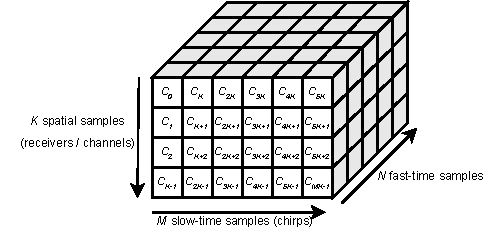
\includegraphics[width=0.9\textwidth]{fig/4/radar-cube.pdf}
    \caption{Radar cube with dimensions corresponding to \gls{cube-z}.}
    \label{fig:radar-cube}
\end{figure}

Using the described transformations, the vector \gls{samples-vec} can be transformed into a 4-dimensional tensor \gls{radarcube-array} given by \ref{eq:radarcube-array}.
The Appendix \ref{app:get_frames} presents an example of parsing the tensor $\vec{S}$ from the \texttt{radar.raw} file using Python and Numpy.

\begin{equation}
    \label{eq:radarcube-array}
    \gls{radarcube-array} = \begin{bmatrix}
        \gls{radarcube-array}_0 &
        \gls{radarcube-array}_1 &
        \gls{radarcube-array}_2 &
        \ldots &
        \gls{radarcube-array}_{| \gls{samples-vec} | \div \gls{numsamples} \gls{numchirps} \gls{numrcv} }
    \end{bmatrix}^{\gls{transpose}}
\end{equation}

To turn the radar data cubes into useful information,
multiple data processing algorithms can be applied to the data.
Since most \gls{har} methods for radar signals use the velocity spectrum,
the most interesting information is the target positions and the corresponding velocity spectra~\cite{sensing-survey}.
The position information can be used to track the targets and get continuous time-Doppler data for a given target.
Additionally, the position information can be used to aid in the microphone beam forming.

Section \ref{sec:range-angle} briefly covers the methods for extracting the range-azimuth information from the radar samples.
Section \ref{sec:cfar} briefly covers the methods for detecting and tracking targets from the data,
and finally, Section \ref{sec:doppler-spectrum} briefly covers the \gls{fft} based algorithm for extracting the Doppler-spectrum.

\subsection{Range-azimuth spectrum}
\label{sec:range-angle}

For extracting the range-azimuth data from the radar signals,
\gls{2d-music} is one of the most attractive methods.
Compared to the traditional \gls{fft} based methods, the \gls{2d-music} can achieve significantly better resolution
in both the angular domain and the range domain~\cite{2d-music-van-rossum}.
A major downside of the \gls{2d-music} algorithm is extremely high computational load and memory usage.
The use of \glspl{fpga} or \glspl{asic} may be used in applications to make the computations faster.

The radar device used in the sensor assembly can be configured to switch between two transmitting antennas,
such that odd chirps are transmitted on a different antenna than even chirps.
If this feature is used, the effective amount of spatial channels in the radar data is $2\gls{numrcv}$,
and each two radar cubes can be combined along the first axis to form another data cube.~\cite{ti-iwr-user-guide}
Based on this, a new tensor $\gls{radarcube-array-other}$ can be defined along a new variable $\gls{numrcv-other}$ that is the number of active receivers.

\begin{align}
    &\begin{cases}
        \forall \gls{framenumber} \in \left[ 0, \frac{ |\gls{samples-vec}| }{2\gls{numsamples}\gls{numchirps}\gls{numrcv}} \right] :
            \gls{radarcube-array-other}(z) = (\gls{radarcube-array}(2z) | \gls{radarcube-array}(2z+1)) \\
        \gls{numrcv-other} = 2\gls{numrcv}
    \end{cases},&&\text{if switching transmitters}
    \\
    &\begin{cases}
        \gls{radarcube-array-other} = \gls{radarcube-array} \\
        \gls{numrcv-other} = \gls{numrcv}
    \end{cases},&&\text{othwerwise}
\end{align}

The tensor augmentation operation $(\vec{A} | \vec{B})$ is defined by the transformation \\
$(\vec{A}^{\gls{numrcv} \times \gls{numchirps} \times \gls{numsamples}}, \vec{B}^{\gls{numrcv} \times \gls{numchirps} \times } \gls{numsamples}) \to \vec{(A|B)}^{2\gls{numrcv} \times \gls{numchirps} \times \gls{numsamples}}$, given by
equation \ref{eq:tensor-augmentation} where the magnitude of each element $|~(\vec{A}|\vec{B})(\gls{rcvnumber}, \gls{chirpnumber})~| = \gls{numsamples}$.

\begin{equation}
\label{eq:tensor-augmentation}
    (\vec{A} | \vec{B}) =
    \begin{bmatrix}
        \vec{A}(0, 0) & \vec{A}(0, 1) & \ldots & \vec{A}(0, M-1) \\
        \vec{A}(1, 0) & \vec{A}(1, 1) & \ldots & \vec{A}(1, M-1) \\
        \vdots        & \vdots        & \ddots & \vdots        \\
        \vec{A}(K-1, 0) & \vec{A}(K-1, 1) & \ldots & \vec{A}(K-1, M-1) \\
        \vec{B}(0, 0) & \vec{B}(0, 1) & \ldots & \vec{B}(0, M-1) \\
        \vec{B}(1, 0) & \vec{B}(1, 1) & \ldots & \vec{B}(1, M-1) \\
        \vdots        & \vdots        & \ddots & \vdots        \\
        \vec{B}(K-1, 0) & \vec{B}(K-1, 1) & \ldots & \vec{B}(K-1, M-1) \\
    \end{bmatrix},
\end{equation}

Similar to \gls{cube-z}, the \gls{framenumber}:th radar cube in \gls{radarcube-array-other} can be denoted by \gls{cube-z-other}.
Using these definitions, the \gls{2d-music} spectrum can be calculated.
The first and third dimension of the tensor \gls{cube-z-other} constitute for the samples recorded during a single dwell,
i.e. a chirp. It can be represented by the tensor \gls{dwell-m}, given by equation \ref{eq:tensor-D}.
The part of the data cube represented by \gls{dwell-m} is highlighted in Figure \ref{fig:tensor-D}.

\begin{equation}
\label{eq:tensor-D}
    \gls{dwell-m} = \begin{bmatrix} \gls{cube-z-other}(0, m) & \gls{cube-z-other}(1, m) & \ldots & \gls{cube-z-other}(K^{\prime}, m)  \end{bmatrix}^{\gls{transpose}}
\end{equation}

\begin{figure}[H]
    \centering
    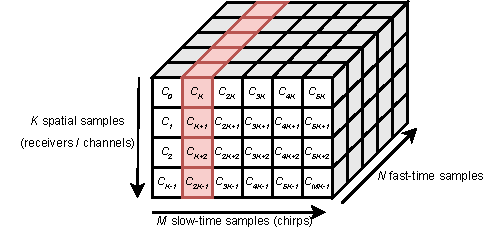
\includegraphics[width=0.8\textwidth]{fig/4/radar-cube-tensor-D.pdf}
    \caption{The part of the radar data cube represented by the tensor \gls{dwell-m} is highlighted in red ($\gls{chirpnumber} = 1$).}
    \label{fig:tensor-D}
\end{figure}

Under the narrowband assumption, the samples of the tensor \gls{dwell-m} can be modeled
as given by equation \ref{eq:sample-approximation}~\cite{music-based-algo}.
The symbols used in the equation  are defined in Table \ref{tab:sample-approximation-variables}.

\begin{equation}
\label{eq:sample-approximation}
\gls{dwell-m} (\gls{rcvnumber}, \gls{samplenumber}) =
    \sum_{\gls{targetnumber}=0}^{\gls{numtargets}-1} \gls{alpha-l} e^{\gls{imag-unit} \gls{phase}} ~
        e^{\gls{imag-unit} 2 \pi \frac{2 \gls{range-l} \gls{bandwidth}}{\gls{lightspeed} \gls{dwell-time} \gls{framerate}} \gls{samplenumber} } ~
        e^{\gls{imag-unit} \frac{2 \pi}{ \gls{wavelen} } \gls{rcv-dist} \gls{rcvnumber} \sin \gls{azimuth-l}}
        + \gls{noise}.
\end{equation}

\begin{table}[]
    \centering
    \begin{tabular}{c l l}
    \toprule
        \textbf{Symbol} & \textbf{Definition} \\
    \midrule
        \gls{rcvnumber} & Index of an antenna in the receiving uniform linear array \\
        \gls{samplenumber} & Index of a fast-time sample in \gls{chirp-m}\\
        \gls{numtargets} & Number of reflecting radar targets \\
        \gls{alpha-l} & Amplitude of the reflected signal from the $l$:th target \\
        $e^{\gls{imag-unit} \gls{phase}}$ & Phase of the reflected signal from the $l$:th target\\
        \gls{range-l} & Range from the receiver to the $l$:th target \\
        \gls{bandwidth} & The bandwidth of the chirp \\
        \gls{samplerate} & Sampling frequency \\
        \gls{lightspeed} & The speed of light \\
        \gls{dwell-time} & Dwell time: $\gls{numsamples} \div \gls{framerate}$\\
        \gls{azimuth-l} & Angle of arrival of the signal reflected from the $l$:th target \\
        $\gls{noise}$ & Additive white Gaussean noise in the \gls{samplenumber}:th sample of the \gls{rcvnumber}:th receiver \\
        \gls{rcv-dist} & The distance between adjacent receivers \\
    \bottomrule
    \end{tabular}
    \caption{Definitions of the symbols used in equation \ref{eq:sample-approximation}.}
    \label{tab:sample-approximation-variables}
\end{table}

The tensor \gls{dwell-m} may also be represented in matrix format as shown by the equations 
\ref{eq:matrix-sample-approximation-1}--\ref{eq:matrix-sample-approximation-6}.

\begin{align}
\label{eq:matrix-sample-approximation-1}
    &\gls{dwell-m} = \gls{angle-matrix}\vec{X}\gls{range-matrix} + \gls{noise-matrix} \\
\label{eq:matrix-sample-approximation-2}
    &\gls{angle-matrix} = \begin{bmatrix} \gls{angle-vector}(\gls{angle-az}_0) & \gls{angle-vector}(\gls{angle-az}_1) \ldots & \gls{angle-vector}(\gls{angle-az}_{\gls{numtargets}-1}) \end{bmatrix}_{\gls{numrcv} \times \gls{numtargets}} \\
\label{eq:matrix-sample-approximation-3}
    &\vec{X} = \begin{bmatrix} \alpha_{0}~e^{\gls{imag-unit}\gls{phase}_{0}} & & & \\ & \alpha_{1}~e^{\gls{imag-unit}\gls{phase}_{1}} & & \\ & & \ddots & \\ & & & \alpha_{L-1}~e^{\gls{imag-unit}\gls{phase}_{\gls{numtargets}-1}} \end{bmatrix}_{\gls{numtargets} \times \gls{numtargets}} \\
\label{eq:matrix-sample-approximation-4}
    &\gls{range-matrix} = \begin{bmatrix} \gls{range-vector}(\gls{range}_0) & \gls{range-vector}(\gls{range}_1) \ldots & \gls{range-vector}(\gls{range}_{\gls{numtargets}-1}) \end{bmatrix}_{\gls{numsamples} \times \gls{numtargets}} \\
\label{eq:matrix-sample-approximation-5}
    &\gls{angle-vector}(\gls{angle-az}_{\gls{targetnumber}}) = \begin{bmatrix} 1 & e^{ \gls{imag-unit} \frac{2 \pi}{ \gls{wavelen} } \gls{rcv-dist} \sin \gls{angle-az}_{\gls{targetnumber}}} & \ldots & e^{ \gls{imag-unit} \frac{2 \pi}{ \gls{wavelen} } \gls{rcv-dist}(\gls{numrcv}-1) \sin \gls{angle-az}_{\gls{targetnumber}}} \end{bmatrix}_{1 \times \gls{numrcv}} \\
\label{eq:matrix-sample-approximation-6}
    &\gls{range-vector}(\gls{range}_{\gls{targetnumber}}) = \begin{bmatrix} 1 & e^{ \gls{imag-unit} 2 \pi \frac{2 \gls{range}_{\gls{targetnumber}} \gls{bandwidth}}{\gls{lightspeed} \gls{dwell-time} \gls{samplerate}} } & \ldots & e^{ \gls{imag-unit} 2 \pi \frac{2 \gls{range}_{\gls{targetnumber}} \gls{bandwidth}}{\gls{lightspeed} \gls{dwell-time} \gls{samplerate}} (\gls{numsamples}-1) } \end{bmatrix}_{1 \times \gls{numsamples}}
\end{align}

Equation \ref{eq:matrix-sample-approximation-1} is equivalent to equation \ref{eq:sample-approximation}.
In equation \ref{eq:matrix-sample-approximation-1}, \gls{angle-matrix} is the angle steering matrix consisting of the steering vectors $\gls{angle-vector}(\theta_0)$ ... $\gls{angle-vector}(\gls{angle-az}_{\gls{numtargets}-1})$.
The matrix \gls{range-matrix} is the range steering matrix which consists of the range steering vectors $\gls{range-vector}(\gls{range}_0)$ ... $\gls{range-vector}(\gls{range}_{\gls{numtargets}-1})$.
The diagonal matrix $\vec{X}$ contains the complex amplitudes and phases of the reflected signals.
Finally, the \gls{noise-matrix} is the additive white Gaussian noise matrix.
Using this information, the \gls{2d-music} algorithm can be applied to calculate the range-azimuth spectrum.

The \gls{2d-music} algorithm is based on evaluation of the covariance matrix of the received signal and the separation of noise and target signal subspaces.
Multiple sweeps (chirps) are typically used for evaluating the covariance matrix.
The noise and target signal subspaces are estimated from the covariance matrix by applying eigenvalue decomposition to the covariance matrix.
The resulting eigenvalues are then used to estimate the number of targets to separate the subspaces.
The \gls{2d-music} spectrum is then estimated from the correlation of the noise subspace
and the range-azimuth steering matrix given by equation \ref{eq:steering-matrix}.~\cite{2d-music-van-rossum}

When the reflected signals are correlated, which is the case when a target spans multiple range or angle bins,
the dimension of the signal subspace is not equal to the number of targets.
This can be solved by applying smoothing techniques, such as \gls{fbss}, to the data.~\cite{2d-music-van-rossum, fbss-techniques}

For a $\gls{numrcv-other} \times \gls{numsamples}$ matrix, the \gls{fbss} algorithm is applied by defining a window with dimensions $\gls{smoothing-wnd-rows} \times \gls{smoothing-wnd-cols}$,
and then scanning the data matrix in all possible positions: 
$\gls{num-smoothing-rows} = \gls{numrcv-other} - \gls{smoothing-wnd-rows}$ positions in the angular dimension and $\gls{num-smoothing-cols} = \gls{numsamples} - \gls{smoothing-wnd-cols}$ positions in the range dimension.
For each scanning position, the sub-matrix is flattened in column-major order to form the vector $\gls{smoothing-vector}(\gls{smoothing-row}, \gls{smoothing-col})$,
where $\gls{smoothing-row} \in \left[ 0, \gls{num-smoothing-cols} \right)$ and $\gls{smoothing-col} \in \left[ 0, \gls{num-smoothing-cols} \right) $.
The vectors $\gls{smoothing-vector}(\gls{smoothing-row}, \gls{smoothing-col})$ are then stacked column-wise to form the spatial-smoothed data matrix \gls{smoothed-matrix}.
The scanning procedure is illustrated in Figure \ref{fig:data-matrix-scanning}.~\cite{2d-music-van-rossum, music-based-algo}

\begin{figure}[H]
    \centering
    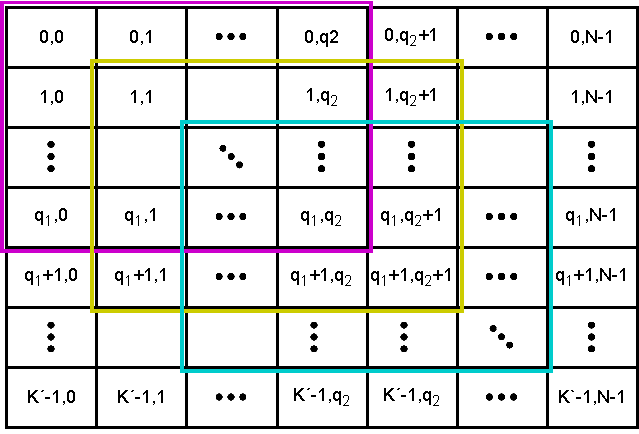
\includegraphics[width=0.67\textwidth]{fig/4/array-scanning.pdf}
    \caption{Scanning window procedure for the data matrix. The matrix is scanned in all possible positions where the $q_1 \times q_2$ window can fit.}
    \label{fig:data-matrix-scanning}
\end{figure}

\begin{equation}
\label{eq:fbss-scanning}
    \gls{smoothed-matrix} = \begin{bmatrix}  \gls{smoothing-vector}(0, 0) & \gls{smoothing-vector}(1, 0) & \ldots & \gls{smoothing-vector}(\gls{num-smoothing-cols}-1, 0) & \gls{smoothing-vector}(0, 1) & \gls{smoothing-vector}(1, 1) \ldots & \gls{smoothing-vector}(\gls{num-smoothing-cols}-1, \gls{num-smoothing-rows}-1) \end{bmatrix}
\end{equation}

The resulting dimensions of \gls{smoothed-matrix} are $\gls{smoothing-wnd-rows}\gls{smoothing-wnd-cols} \times \gls{num-smoothing-rows}\gls{num-smoothing-cols}$.
The vectors $\gls{smoothing-vector}(\gls{smoothing-row}, \gls{smoothing-col})$ are given by equation \ref{eq:scanning}.

\begin{equation}
    \label{eq:scanning}
    \gls{smoothing-vector}(\gls{smoothing-row}, \gls{smoothing-col})
    = \begin{bmatrix} 
        \gls{dwell-m}(\gls{smoothing-row},         \gls{smoothing-col}) \\
        \gls{dwell-m}(\gls{smoothing-row}+1,       \gls{smoothing-col}) \\
        \vdots \\
        \gls{dwell-m}(\gls{smoothing-row}+\gls{smoothing-wnd-rows}-1, \gls{smoothing-col}) \\
        \gls{dwell-m}(\gls{smoothing-row},         \gls{smoothing-col}+1) \\
        \gls{dwell-m}(\gls{smoothing-row}+1,       \gls{smoothing-col}+1) \\
        \vdots \\
        \gls{dwell-m}(\gls{smoothing-row}+\gls{smoothing-wnd-rows}-1, \gls{smoothing-col}+\gls{smoothing-wnd-cols}-1)
    \end{bmatrix}_{\gls{smoothing-wnd-rows}\gls{smoothing-wnd-cols} \times 1}
\end{equation}

Having formed the smoothed data matrix \gls{smoothed-matrix}, the data smoothed covariance matrix \gls{covariance-smoothed-matrix} 
can then be evaluated as given by equation \ref{eq:covariance-matrix}.
The matrix $\vec{J}$ in equation \ref{eq:covariance-matrix} is the transition matrix defined by equation \ref{eq:transition-matrix}.
\cite{2d-music-van-rossum, fbss-techniques}

\begin{equation}
    \label{eq:covariance-matrix}
    \gls{covariance-smoothed-matrix} =
        \frac{1}{2 \gls{num-smoothing-rows}\gls{num-smoothing-cols} }
        \left[
            \gls{smoothed-matrix} \gls{smoothed-matrix}^{\gls{hermitian}}
            + \vec{J}( \gls{smoothed-matrix} \gls{smoothed-matrix}^{\gls{hermitian}} )^{\gls{conjugate}}\vec{J} 
        \right]
\end{equation}

\begin{equation}
    \label{eq:transition-matrix}
    J = \begin{bmatrix}
        0      & 0      & \ldots & 1      \\
        \vdots & 0      & 1      & 0      \\
        0      & \iddots & 0      & \vdots \\
        1      & 0      & \ldots & 0      \\
    \end{bmatrix}_{\gls{smoothing-wnd-rows}\gls{smoothing-wnd-cols} \times \gls{smoothing-wnd-rows}\gls{smoothing-wnd-cols}}
\end{equation}

To estimate the signal and noise subspaces, the mean of the covariance matrices of multiple sweeps is used.
The final covariance matrix used for the eigenvalue decomposition is given by equation \ref{eq:mean-covariance-matrix}.
\cite{music-based-algo}

\begin{equation}
    \label{eq:mean-covariance-matrix}
    \gls{cov-matrix} = \frac{1}{\gls{numchirps}} \sum_{\gls{chirpnumber}=0}^{\gls{numchirps}-1} \gls{covariance-smoothed-matrix}
\end{equation}

The covariance matrix \gls{cov-matrix} can be factorized as

\begin{equation}
    \gls{cov-matrix} = \gls{eigvecs} \gls{eigvals} \gls{eigvecs}^{\gls{hermitian}},
\end{equation}

where \gls{eigvecs} contains the eigenvectors of \gls{cov-matrix} and \gls{eigvals} is a diagonal matrix containing the corresponding eigenvalues.
Given the number of targets \gls{numtargets} (equations \ref{eq:num-targets}--\ref{eq:music-mdl}),
the noise subspace \gls{noisespace} with dimensions $\gls{smoothing-wnd-rows}\gls{smoothing-wnd-cols} \times \gls{num-smoothing-rows}\gls{num-smoothing-cols} - \gls{numtargets}$
can be partitioned from \gls{eigvecs} as shown by equation \ref{eq:noise-subspace-partition}~\cite{2d-music-van-rossum}.

\begin{equation}
    \label{eq:noise-subspace-partition}
    \gls{noisespace} = \begin{bmatrix} \gls{eigvecs}(\gls{numtargets}) & \ldots & \gls{eigvecs}(\gls{num-smoothing-rows}\gls{num-smoothing-cols} - 1) \end{bmatrix}
\end{equation}

The number of targets \gls{numtargets} can be estimated using information theoretic criteria, such as \gls{aic} or \gls{mdl}.
As proposed by Wax and Kailath, equation \ref{eq:music-aic} shows the formula for \gls{aic} for this problem
and equation \ref{eq:music-mdl} shows the formula for \gls{mdl}.
For both equations, the number of targets is the argument of the minimum for the criteria (Equation \ref{eq:num-targets}).
\cite{wax-kailath-85}

\begin{equation}
    \label{eq:num-targets}
    \gls{numtargets} = \argmin\limits_{0\,\leq\,\gls{targetnumber}\,<\,\gls{smoothing-wnd-rows}\gls{smoothing-wnd-cols}q_{1}q_{2}}\, \mathrm{AIC}(\gls{targetnumber}) \quad \vee \quad \gls{numtargets} = \argmin\limits_{0\,\leq\,\gls{targetnumber}\,<\,\gls{smoothing-wnd-rows}\gls{smoothing-wnd-cols}}\, \mathrm{MDL}(\gls{targetnumber})
\end{equation}

\begin{equation}
    \label{eq:music-aic}
    \mathrm{AIC}(\gls{targetnumber}) = -2 \log \left(
        \frac
            {\prod\limits_{i = \gls{targetnumber}}^{\gls{smoothing-wnd-rows}\gls{smoothing-wnd-cols}-1} \Lambda(i,i)^{1 \div (\gls{smoothing-wnd-rows}\gls{smoothing-wnd-cols} - \gls{targetnumber})}} 
            {\frac{1}{\gls{smoothing-wnd-rows}\gls{smoothing-wnd-cols}-k} \sum\limits_{i=\gls{targetnumber}}^{\gls{smoothing-wnd-rows}\gls{smoothing-wnd-cols}-1} \gls{eigvals}(i,i)}
    \right)^{(\gls{smoothing-wnd-rows}\gls{smoothing-wnd-cols}-\gls{targetnumber})\gls{numrcv}} + 2\gls{targetnumber}(2\gls{smoothing-wnd-rows}\gls{smoothing-wnd-cols}-\gls{targetnumber})
\end{equation}

\begin{equation}
    \label{eq:music-mdl}
    \mathrm{MDL}(\gls{targetnumber}) = - \log \left( 
        \frac
            {\prod\limits_{i = \gls{targetnumber}}^{\gls{smoothing-wnd-rows}\gls{smoothing-wnd-cols}-1} \Lambda(i,i)^{1 \div (\gls{smoothing-wnd-rows}\gls{smoothing-wnd-cols} - \gls{targetnumber})}} 
            {\frac{1}{\gls{smoothing-wnd-rows}\gls{smoothing-wnd-cols}-\gls{targetnumber}} \sum\limits_{i=\gls{targetnumber}}^{\gls{smoothing-wnd-rows}\gls{smoothing-wnd-cols}-1} \Lambda(i,i)}
    \right)^{(\gls{smoothing-wnd-rows}\gls{smoothing-wnd-cols}-\gls{targetnumber})\gls{numrcv}} + \frac{1}{2}\gls{targetnumber}(2\gls{smoothing-wnd-rows}\gls{smoothing-wnd-cols}-l) \log \gls{numrcv}
\end{equation}

Having estimated the noise subspace, the \gls{2d-music} spectrum $\gls{power}(\gls{range}, \gls{angle-az})$ is given by equation \ref{eq:2d-music-spectrum}.
The range-azimuth steering matrix $\gls{steering}(\gls{angle-az}, \gls{range})$ is given by equation \ref{eq:steering-matrix},
where $\gls{angle-vector}(\gls{angle-az})$ and $\gls{range-vector}(\gls{range})$ are given by 
equations \ref{eq:matrix-sample-approximation-5} and \ref{eq:matrix-sample-approximation-6} respectively.~\cite{music-based-algo}

\begin{equation}
    \label{eq:2d-music-spectrum}
    \gls{power}(\gls{range}, \gls{angle-az}) = \frac{1}{ \gls{steering}(\gls{angle-az}, \gls{range})^{\gls{hermitian}} \gls{noisespace} \gls{noisespace}^{\gls{hermitian}} \gls{steering}(\gls{angle-az}, \gls{range}) }
\end{equation}

\begin{equation}
    \label{eq:steering-matrix}
    \gls{steering}(\gls{angle-az}, \gls{range}) = \gls{angle-vector}(\gls{angle-az}) \otimes \gls{range-vector}(\gls{range})
\end{equation}

An example implementation of the \gls{fbss} algorithm is provided in Appendix \ref{app:fbss-algorithm}
and an example implementation of the \gls{2d-music} algorithm is provided in Appendix \ref{app:2d-music-algorithm}.
Figure \ref{fig:2d-music-example} shows an example graph of a \gls{2d-music} spectrum.

\begin{figure}
    \centering
    \begin{subfigure}[b]{0.49\textwidth}
        \centering
        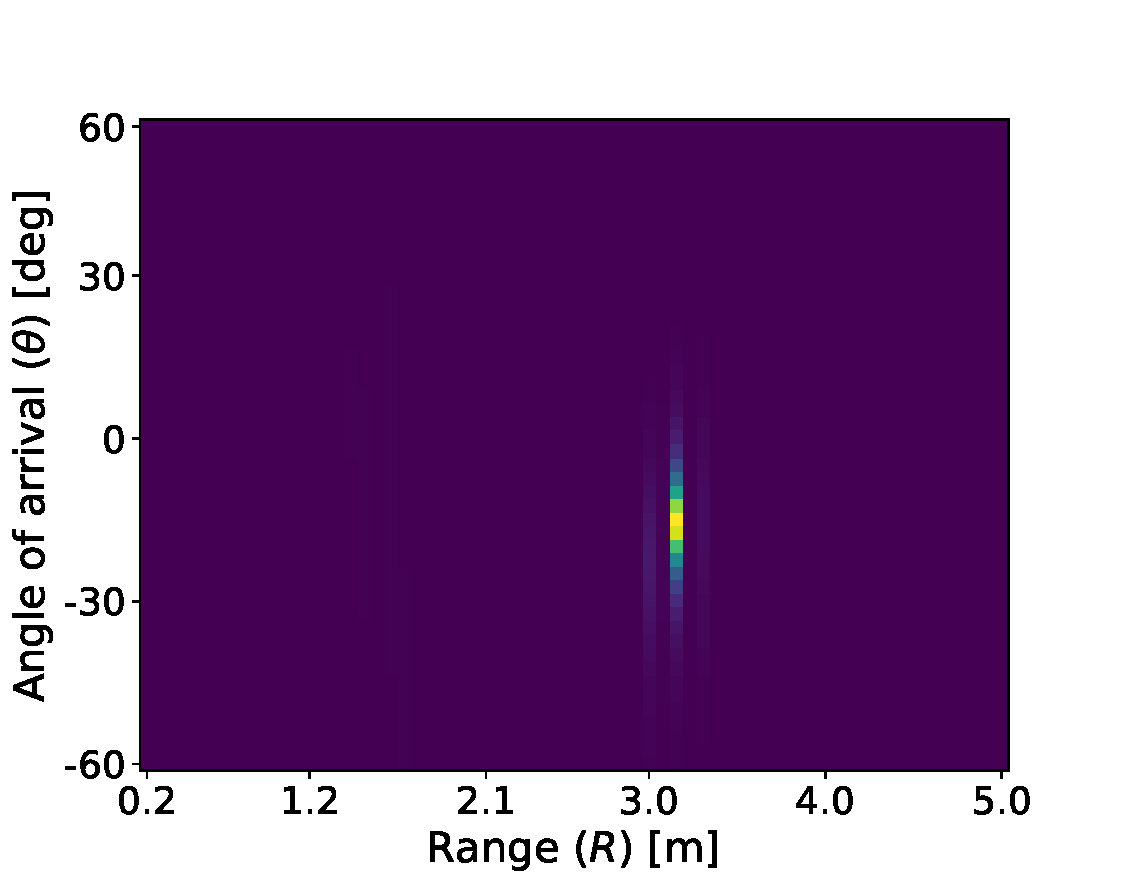
\includegraphics[width=\textwidth]{fig/4/music_spectrum.pdf}
        \caption{2D-MUSIC spectrum.}
    \end{subfigure}
    \hfill
    \begin{subfigure}[b]{0.49\textwidth}
        \centering
        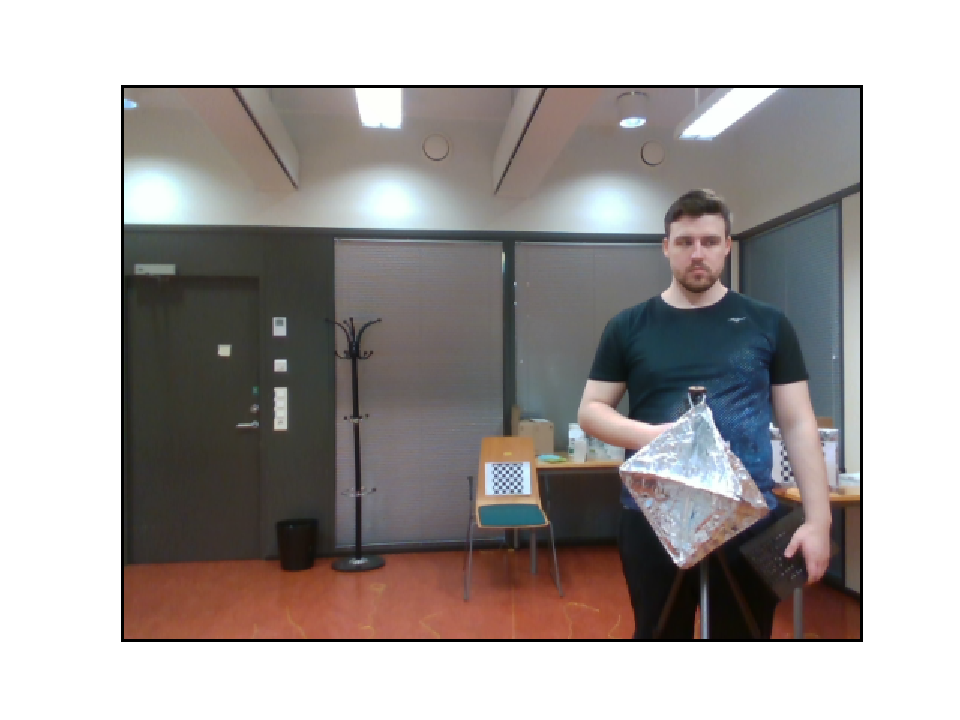
\includegraphics[width=\textwidth]{fig/4/music_corresponding_rgb_image.pdf}
        \caption{Corresponding RGB video frame.}
    \end{subfigure}
    \caption{2D-MUSIC spectrum and a corresponding RGB video frame.}
    \label{fig:2d-music-example}
\end{figure}

\subsection{Range-velocity spectrum}
\label{sec:doppler-spectrum}
When the range of a target changes by less than half-wavelength,
or the propagation distance changes by less than one wavelength,
the phase-shift in the received reflection is linearly proportional to the change in distance.
Because the time between two samples is known,
the change in phase between two samples is therefore proportional to the velocity of the target.
When the velocity of the target $\gls{velocity} \ll \frac{\gls{lightspeed}\gls{numchirps}}{\gls{txfreq} \gls{chirptime}}$,
the relation between the phase shift (\gls{phase-change}) and velocity (\gls{velocity}) is given by equation \ref{eq:phase-velocity-relation}
(derived in Appendix \ref{app:deriving-range-velocity-fft}),
where \gls{chirptime} is the chirp cycle time, \gls{txfreq} is the frequency of the transmitted signal and \gls{lightspeed} is the speed of light.

\begin{equation}
    \label{eq:phase-velocity-relation}
    \gls{phase-change} = \frac{4 \pi \gls{txfreq} \gls{velocity} \gls{chirptime}}{\gls{lightspeed}}
\end{equation}

The equation \ref{eq:phase-velocity-relation} could be used to create a velocity steering vector
and the \gls{2d-music} algorithm could applied to acquire the range-velocity spectrum.
The \gls{music} algorithm is computationally very demanding, though.
By taking multiple samples of the signal, a sufficient resolution can be had
for the range--velocity spectrum with \gls{2d-fft} method,
which is computationally much faster.

Given the signal is sampled $\gls{numsamples}$ times per each of the $\gls{numchirps}$ chirps on $\gls{numrcv}$ channels,
the dimensions of the resulting data cube are $\gls{numrcv} \times \gls{numchirps} \times \gls{numsamples}$ (Section \ref{sec:radar-data}).
For the \gls{2d-fft} method,
the range and velocity resolutions (\gls{range-resolution} and \gls{velocity-resolution} respectively),
the maximum range (\gls{maxrange}),
and the minimum and maximum velocities 
(\gls{minvelocity}and \gls{maxvelocity} respectively) are given by equations
\ref{eq:2dfft-range-resolution}--\ref{eq:2dfft-min-max-velocity}
(derived in Appendix \ref{app:deriving-range-velocity-fft}).

\begin{equation}
    \label{eq:2dfft-range-resolution}
    \gls{range-resolution} = \frac{\gls{samplerate} \gls{lightspeed}}{2\gls{numsamples}\gls{slope}}
\end{equation}
\begin{equation}
    \label{eq:2dfft-velocity-resolution}
    \gls{velocity-resolution} = \frac{\gls{lightspeed}}{2 \gls{numchirps} \gls{txfreq} \gls{chirptime}}
\end{equation}
\begin{equation}
    \label{eq:2dfft-max-range}
    \gls{maxrange} = \frac{\gls{samplerate} \gls{lightspeed}}{2 \gls{slope}}
\end{equation}
\begin{equation}
    \label{eq:2dfft-min-max-velocity}
    \gls{minvelocity} = -\gls{maxvelocity} = \frac{\gls{lightspeed}}{4 \gls{txfreq} \gls{chirptime}} \\
\end{equation}

The range-velocity spectrum is calculated by first averaging the data
cube corresponding to the \gls{framenumber}:th frame (\gls{cube-z})
along the first axis (receivers) to increase the \gls{snr},
which will result in the data matrix \gls{mean-chirp-matrix}, as given by equation \ref{eq:fft-snr-boost}.
The dimensions of \gls{mean-chirp-matrix} are $\gls{numchirps} \times \gls{numsamples}$.

\begin{equation}
    \label{eq:fft-snr-boost}
    \gls{mean-chirp-matrix}(\gls{chirpnumber}, \gls{samplenumber}) = \sum \limits_{\gls{rcvnumber} = 0}^{\gls{numrcv}-1} \gls{cube-z}(\gls{rcvnumber}, \gls{chirpnumber}, \gls{samplenumber})
\end{equation}

After calculating \gls{mean-chirp-matrix}, the Fourier transform is performed on the second axis of the matrix,
which is the fast-time samples. Denoting $\gls{mean-chirp-matrix} = \begin{bmatrix} \gls{fast-samples}(0) & \gls{fast-samples}(1) & \ldots & \gls{fast-samples}(\gls{numchirps}-1) \end{bmatrix}$,
where $\gls{fast-samples}(\gls{chirpnumber})$ is the vector containing the fast-time samples for the $\gls{chirpnumber}$:th chirp,
the operation is given by equation \ref{eq:fast-time-fft}.

\begin{equation}
    \label{eq:fast-time-fft}
    \gls{range-spectrum}(\gls{chirpnumber}) = \mathcal{F} \left\{ \gls{fast-samples}(\gls{chirpnumber}) \right\}
\end{equation}

The operation $\mathcal{F} \{ \cdot \}$ in equation \ref{eq:fast-time-fft} is the discrete Fourier transform.
The resulting vector $\vec{\hat p}$ has contains the Fourier transform of $\gls{fast-samples}(\gls{chirpnumber})$ as its $\gls{chirpnumber}$:th element.
Each bin in the vectors \gls{range-spectrum} corresponds to a range as given by equation \ref{eq:fast-time-fft-range}.
The function $\gls{range}(\gls{samplenumber})$ gives the corresponding range for the \gls{samplenumber}:th bin in vector $\gls{range-spectrum}(\gls{chirpnumber})$ (Appendix \ref{app:deriving-range-velocity-fft}).

\begin{equation}
    \label{eq:fast-time-fft-range}
    \gls{range}(\gls{samplenumber}) = \gls{samplenumber} \gls{range-resolution} = \frac{\gls{samplenumber} \gls{samplerate} \gls{lightspeed}}{2\gls{numsamples}\gls{slope}}
\end{equation}

Assuming the range of the target changes by less than half a wavelength between two chirps,
the phase difference between the $\gls{samplenumber}$:th element (frequency component) of vectors $\gls{range-spectrum}(\gls{chirpnumber})$ and $\gls{range-spectrum}(\gls{chirpnumber}+1)$
is dictated by the distance the target has moved (Appendix \ref{app:deriving-range-velocity-fft}).
Thus, denoting $\gls{range-spectrum-matrix} = \begin{bmatrix} \gls{range-spectrum}(0) & \gls{range-spectrum}(1) \ldots & \gls{range-spectrum}(\gls{numchirps}-1) \end{bmatrix}^{\gls{transpose}}$,
the Fourier transform can be applied along the first dimension of \gls{range-spectrum-matrix} to acquire the velocities of the targets.
The range-velocity power-spectrum can thus be denoted as 
\gls{range-velocity-unshifted} as given by equation \ref{eq:slow-time-fft-matrix},
where $\gls{velocity-spectrum}(\gls{samplenumber})$ is the velocity spectrum for the \gls{samplenumber}:th range bin, as given by equation \ref{eq:slow-time-fft}.

\begin{equation}
    \label{eq:slow-time-fft-matrix}
    \gls{range-velocity-unshifted} = \begin{bmatrix} \gls{velocity-spectrum}(0) & \gls{velocity-spectrum}(1) & \ldots & \gls{velocity-spectrum}(\gls{numsamples}-1)\end{bmatrix}
\end{equation}

\begin{equation}
    \label{eq:slow-time-fft}
    \gls{velocity-spectrum}(\gls{samplenumber}) = \mathcal{F} \left \{ \begin{bmatrix} \gls{range-spectrum-matrix}(0, \gls{samplenumber}) & \gls{range-spectrum-matrix}(1, \gls{samplenumber}) & \ldots \gls{range-spectrum-matrix}(\gls{numchirps}-1, \gls{samplenumber}) \end{bmatrix}^T \right \}
\end{equation}

Because the velocity can be either positive or negative, the matrix $\gls{range-velocity-unshifted}$ still needs to be shifted so
that the zero-velocity bin is in the center.
The shifted range-velocity spectrum can be defined as $\gls{power}$ as given by equation \ref{eq:fft-shift}.

\begin{equation}
    \label{eq:fft-shift}
    \begin{cases}
        \forall \gls{chirpnumber} < \frac{\gls{numchirps}}{2} :   \gls{power}(\gls{chirpnumber}, \gls{samplenumber}) = \gls{range-velocity-unshifted}(\gls{chirpnumber} + \frac{\gls{numchirps}}{2}, \gls{samplenumber}) \\
        \forall \gls{chirpnumber} \ge \frac{\gls{numchirps}}{2} : \gls{power}(\gls{chirpnumber}, \gls{samplenumber}) = \gls{range-velocity-unshifted}(\gls{chirpnumber} - \frac{\gls{numchirps}}{2}, \gls{samplenumber}) \\
    \end{cases}
\end{equation}

The velocity corresponding to the $\gls{chirpnumber}$:th bin on the first axis of $\gls{power}$ ($\gls{velocity}(\gls{chirpnumber})$) can be calculated from the 
minimum velocity and velocity resolution (equations \ref{eq:2dfft-min-max-velocity} and \ref{eq:2dfft-max-range}).
The velocity $\gls{velocity}(\gls{chirpnumber})$ is given by equation \ref{eq:slow-time-fft-bin-velocity}.

\begin{equation}
    \label{eq:slow-time-fft-bin-velocity}
    \gls{velocity}(\gls{chirpnumber}) = -\frac{\gls{lightspeed}}{4 \gls{txfreq} \gls{chirptime}} + \frac{\gls{chirpnumber} \gls{lightspeed}}{2 \gls{numchirps} \gls{txfreq} \gls{chirptime}}
\end{equation}

Therefore, the matrix $\gls{power}$ contains the range-velocity spectrum of the radar cube.
The power of the reflection in element $\gls{power}(\gls{samplenumber}, \gls{chirpnumber})$ is the absolute value of the element,
whereas the range and velocity are given by equations 
\ref{eq:fast-time-fft-range} and \ref{eq:slow-time-fft-bin-velocity} respectively.
Figure \ref{fig:range-velocity-unfiltered} shows an example range-velocity spectrum
and Figure \ref{fig:range-velocity-rgb} shows the corresponding RGB image.
The target is walking away from the sensor, thus the velocity is negative.

\begin{figure}[H]
    \centering
    \begin{subfigure}[b]{0.49\textwidth}
        \centering
        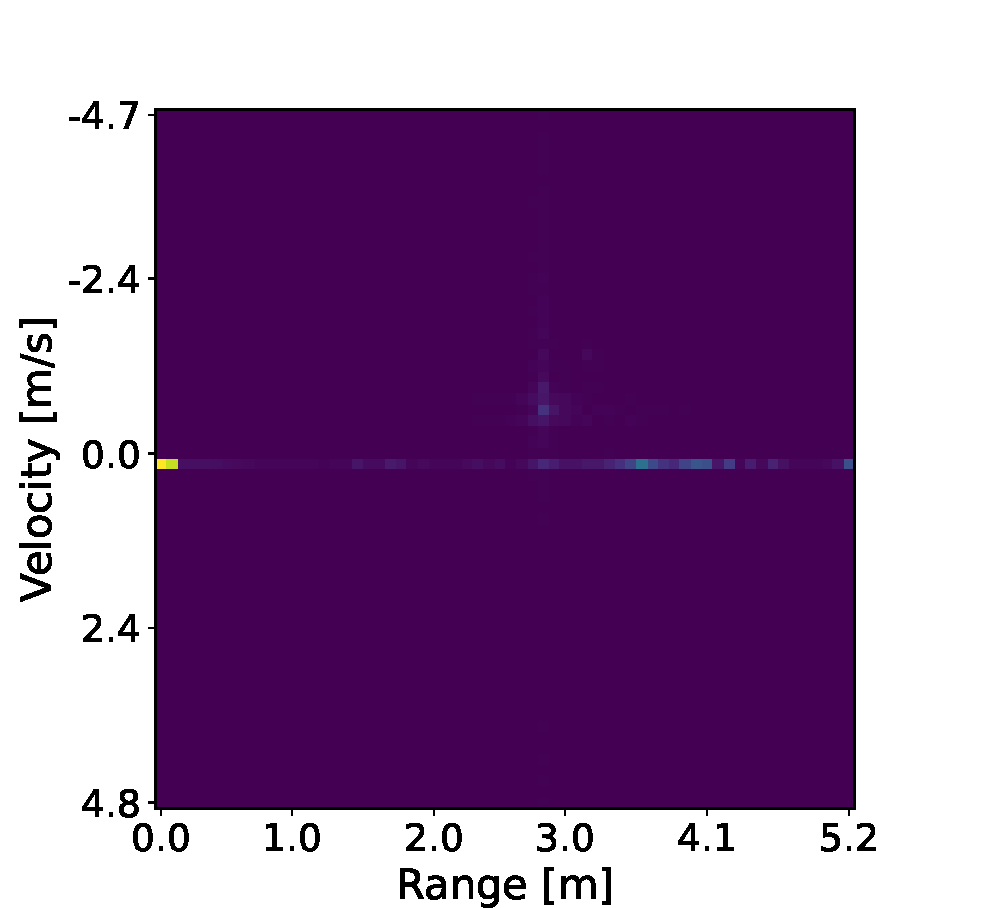
\includegraphics[width=\textwidth]{fig/4/range-velocity.pdf}
        \caption{Range-velocity spectrum (2D-FFT).}
        \label{fig:range-velocity-unfiltered}
    \end{subfigure}
    \hfill
    \begin{subfigure}[b]{0.49\textwidth}
        \centering
        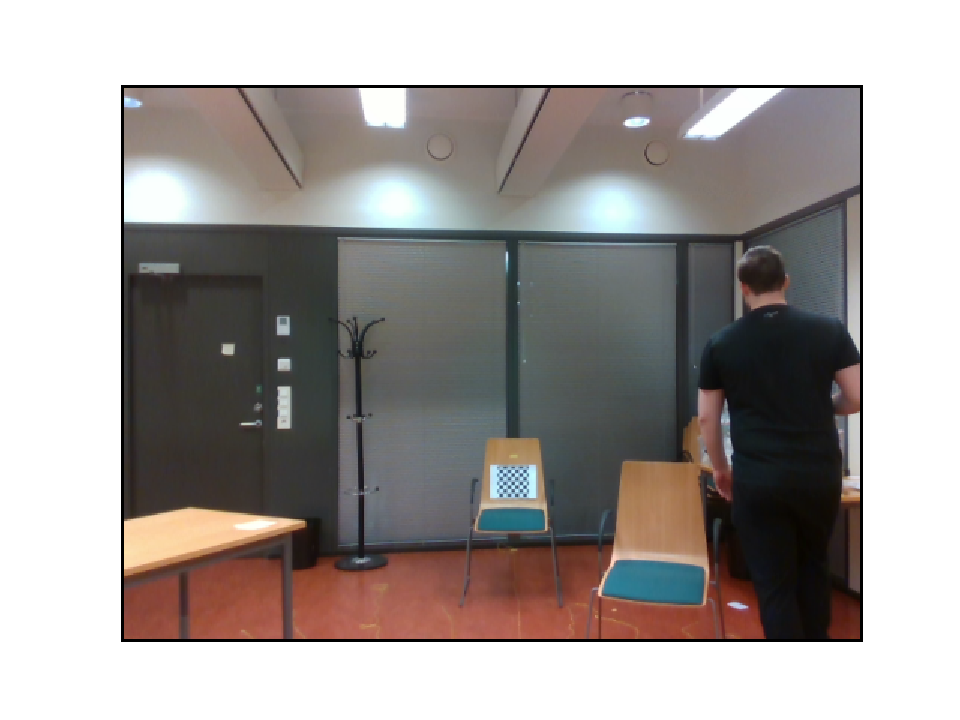
\includegraphics[width=\textwidth]{fig/4/range-velocity-rgb.pdf}
        \caption{Corresponding RGB video frame.}
        \label{fig:range-velocity-rgb}
    \end{subfigure}
    \caption{
        Range-velocity spectrum and the corresponding RGB video frame.
    }
\end{figure}

It is seen from Figure \ref{fig:range-velocity-unfiltered} that there is a lot of power on the near-zero range and in the zero-velocity bins.
The near-zero range power is caused mainly by self-interference in the radar and reflections of static nearby targets.
Static clutter appears in the zero-velocity bins.
The first few range bins should always be muted and if only moving targets are of interest,
also the zero-velocity bins should be muted.

Muting the bins can be done by defining vectors \gls{range-muting-vec} and \gls{velo-muting-vec} of magnitudes $\gls{numsamples}$ and $\gls{numchirps}$ respectively,
where $\gls{range-muting-vec}(\gls{samplenumber})$ is the amplification of the $\gls{samplenumber}$:th range bin
and $\gls{velo-muting-vec}(\gls{chirpnumber})$ is the amplification of the $\gls{chirpnumber}$:th velocity bin.
Corresponding diagonal matrices $\gls{range-muting-matrix}$ and $\gls{velo-muting-matrix}$ can then be defined with the elements
of $\gls{range-muting-vec}$ and $\gls{velo-muting-vec}$ along their diagonals.
Given a minimum range of interest $\gls{minrange}$,
the vectors $\gls{range-muting-vec}$ and $\gls{velo-muting-vec}$ can be defined via equations
\ref{eq:range-coefficients} and \ref{eq:velocity-coefficients}.
The only velocity bins that are muted are the ones corresponding to zero-velocity.

\begin{equation}
\label{eq:range-coefficients}
    \begin{cases}
        \forall \gls{samplenumber} \leq \left \lfloor \frac{ \gls{minrange} }{ \gls{range-resolution} } \right \rfloor :
            \gls{range-muting-vec}(\gls{samplenumber}) = 0 \\
        \forall \gls{samplenumber} > \left \lfloor \frac{ \gls{minrange} }{ \gls{range-resolution} } \right \rfloor :
            \gls{range-muting-vec}(\gls{samplenumber}) = 1
    \end{cases}
\end{equation}

\begin{equation}
\label{eq:velocity-coefficients}
    \begin{cases}
        \forall \gls{chirpnumber} = \frac{1}{2}\gls{numchirps} :
            \gls{velo-muting-vec}(\gls{chirpnumber}) = 0 \\
        \forall \gls{chirpnumber} \neq \frac{1}{2}\gls{numchirps} :
            \gls{velo-muting-vec}(\gls{chirpnumber}) = 1
    \end{cases}
\end{equation}

Having defined the matrices $\gls{range-muting-matrix}$ and $\gls{velo-muting-matrix}$ according to equations
\ref{eq:range-coefficients} and \ref{eq:velocity-coefficients},
the muting of the unwanted bins is achieved by multiplying the matrix
$\gls{power}$ with matrices $\gls{range-muting-matrix}$ and $\gls{velo-muting-matrix}$ as given by equation \ref{eq:2dfft-attenuation}.
The Figure \ref{fig:range-velocity-spectrum-filtered} shows the velocity spectrum 
from Figure \ref{fig:range-velocity-unfiltered}, but with only the zero-range noise filtered 
in Figure \ref{fig:range-velocity-range-filtered} and both zero-range noise and zero-velocity clutter
filtered in Figure \ref{fig:range-velocity-both-filtered}.

\begin{equation}
    \label{eq:2dfft-attenuation}
    \gls{power-filtered} = \gls{velo-muting-matrix} ( \gls{range-muting-matrix} \gls{power}^{\gls{transpose}} )^{\gls{transpose}}
\end{equation}

\begin{figure}[H]
    \centering
    \begin{subfigure}[b]{0.49\textwidth}
        \centering
        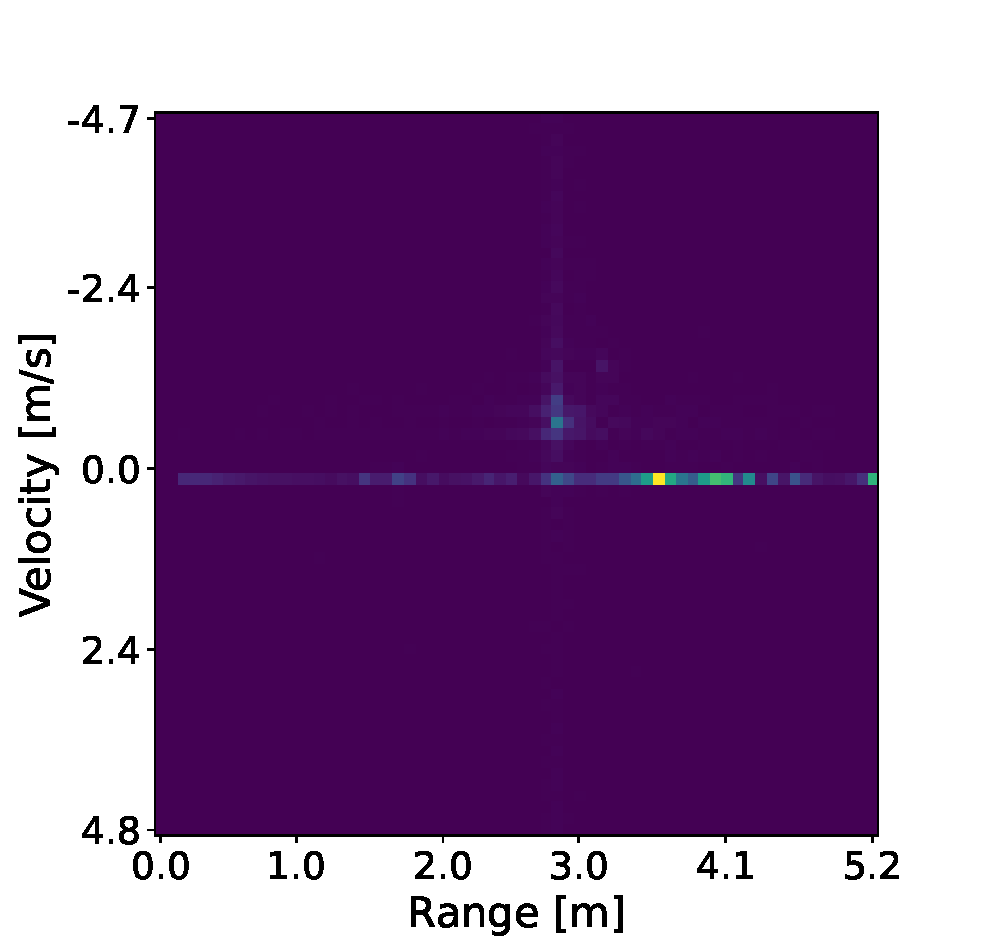
\includegraphics[width=\textwidth]{fig/4/range-velocity-range-filtered.pdf}
        \caption{Range-velocity spectrum with only zero-range noise filtered.}
        \label{fig:range-velocity-range-filtered}
    \end{subfigure}
    \hfill
    \begin{subfigure}[b]{0.49\textwidth}
        \centering
        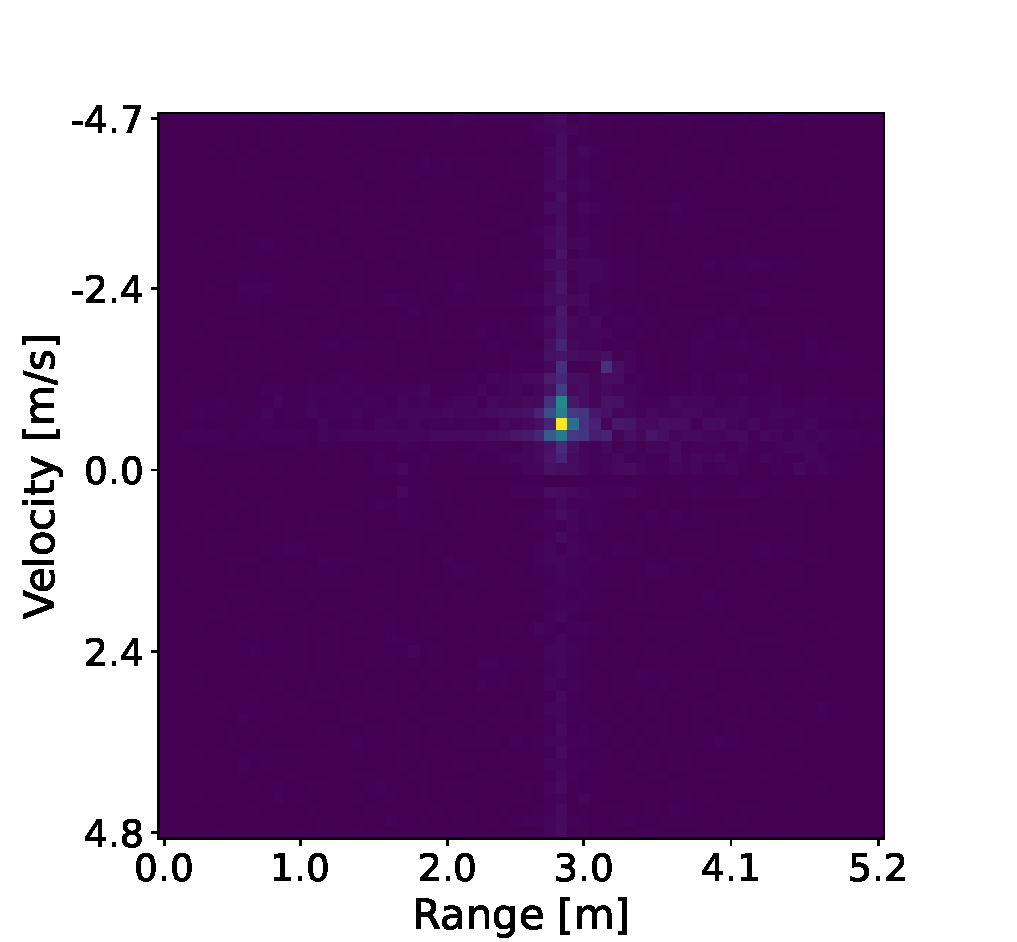
\includegraphics[width=\textwidth]{fig/4/range-velocity-both-filtered.pdf}
        \caption{Range-velocity spectrum with zero-range noise and zero-velocity clutter filtered.}
        \label{fig:range-velocity-both-filtered}
    \end{subfigure}
    \caption{Filtered range-velocity spectrum.}
    \label{fig:range-velocity-spectrum-filtered}
\end{figure}

An example implementation of the \gls{2d-fft} algorithm for acquiring and filtering the range-velocity spectrum
is presented in Appendix \ref{app:2dfft-range-velocity-example}. The example is written in Python.

\subsection{Target detection and tracking}
\label{sec:cfar}
From the calculated spectra, targets can be detected using target detection algorithms.
The most common way of detecting targets from the spectra is picking a threshold and checking if the power a cell is over it.
The threshold be picked in such a way that is higher than the noise power to minimize false positives.
The threshold must also be lower than the power reflected from targets in order to detect true positives. 
In other words, the threshold must be picked in such a way that the error rate is minimized, as illustrated by Figure \ref{fig:error-matrix}.

\begin{figure}
    \centering
    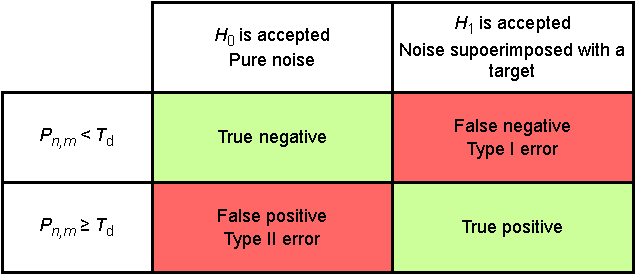
\includegraphics{fig/4/error-matrix.pdf}
    \caption{Different kinds of detection errors. The signal power in the test cell is denoted as $\gls{cell-power}$, whereas $\gls{threshold}$ is the detection threshold.}
    \label{fig:error-matrix}
\end{figure}

Formally, the target detection is done via hypothesis testing, where \gls{null-hypothesis} is that the cell contains only noise
and \gls{alt-hypothesis} is that the cell contains noise superimposed with a target.
When the power of the tested cell is denoted as \gls{cell-power} and detection threshold as $\gls{threshold}$,
the hypothesis test is defined by equation \ref{eq:hypothesis-test}.

\begin{equation}
    \label{eq:hypothesis-test}
    \begin{cases}
        \gls{null-hypothesis}: \gls{cell-power} < \gls{threshold} \\
        \gls{alt-hypothesis}: \gls{cell-power} \ge \gls{threshold}
    \end{cases}
\end{equation}

The threshold depends on parameters of the noise-only distribution.
If the noise distribution was completely known prior to testing,
picking a correct detection threshold would be a trivial task.
In real-world applications the noise spectrum is space-time variant and therefore cannot be known a priori.
This leaves two choices for picking the detection threshold:
using distribution-free detection procedures~\cite{distribution-free-detection} 
or estimating the noise spectrum and using an adaptive algorithm~\cite{mean-level-detection}.

Typically a category of adaptive algorithms called \gls{cfar} detection algorithms is applied for detecting the targets.
The principle of \gls{cfar} algorithms is that the noise distribution is estimated from the calculated spectra (e.g. range-velocity or range-azimuth),
whereof the probability distribution for noise power is estimated.
The detection threshold is picked from the estimated noise probability distribution
based on a predefined probability of a false alarm, thus giving a false alarm rate that is constant.

When the probability density function for noise power in cell $y$ is denoted as $f_{\gls{noise-power}}(y)$,
the probability that \gls{null-hypothesis} is rejected
is given by the Neyman-Pearson criterion (equation \ref{eq:neyman-pearson})~\cite{fast-two-dimensional-cfar, neyman-pearson}.
The criterion is illustrated by Figure \ref{fig:neyman-pearson}.

\begin{equation}
    \label{eq:neyman-pearson}
    \gls{p-fa} = \gls{probability}(\gls{noise-power} \ge \gls{threshold}) = \int_{\gls{threshold}}^{\infty} f_{\gls{noise-power}}(y)dy
\end{equation}

\begin{figure}
    \centering
    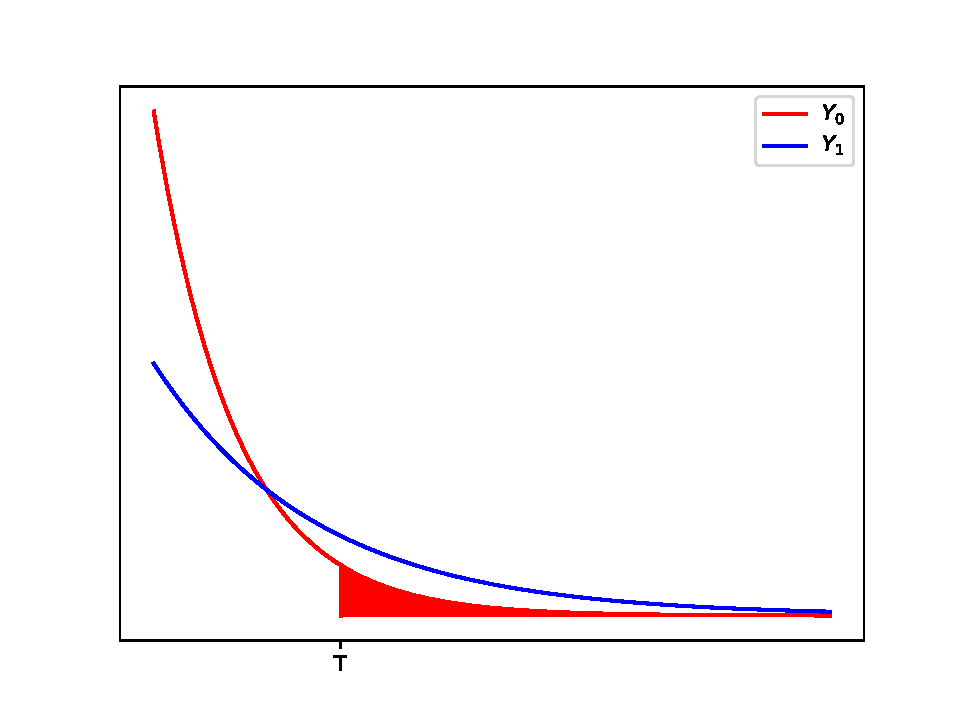
\includegraphics[width=0.67\textwidth]{fig/4/neyman-pearson.pdf}
    \caption{
        The probability density functions for the noise power $\gls{noise-power}$ and signal power $\gls{sig-power}$.
        The highlighted area is the probability of a false alarm as given by equation \ref{eq:neyman-pearson}
        for given decision threshold $\gls{threshold}$.
    }
    \label{fig:neyman-pearson}
\end{figure}

When a square law detector is used for detecting targets in the signal,
i.e. the power of the signal is used as decision criterion,
and the noise in each cell is narrowband Gaussian noise,
the probability distribution for noise follows the exponential distribution.
Thus, the decision threshold $\gls{threshold}$ is given by the quantile function of the exponential distribution (equation \ref{eq:exponential-quantile-func}),
where $\gls{mean-pwr}$ is the average noise power.~\cite{mean-level-detection}

\begin{equation}
    \label{eq:exponential-quantile-func}
    \gls{threshold} = -\gls{mean-pwr} \cdot \ln( 1-\gls{p-fa} )
\end{equation}

Different \gls{cfar} algorithms differ from each other in how the mean noise power $\gls{mean-pwr}$ is estimated.
The \gls{ca} \gls{cfar} algorithm assumes that the noise power in each cell independent and identically distributed.
Based on the central limit theorem, the average noise power may be estimated by defining a window with sufficiently large dimensions,
and calculating the average power in the cells inside the window, disregarding the test cell and some guard cells around it.
This method is based on the assumption that the average noise power is calculated from cells that have a very high likelihood of containing purely noise.
The assumption is fair when the targets are sparse.

The estimated average noise power $\gls{est-mean-pwr}$ around the cell $(\gls{samplenumber}, \gls{chirpnumber})$
in the \gls{ca}-\gls{cfar} algorithm is given by the equation \ref{eq:ca-cfar-noise-estimate}.
The term $\gls{cfar-wnd-sum}(\gls{samplenumber}, \gls{chirpnumber})$ and $\gls{guard-wnd-sum}(\gls{samplenumber}, \gls{chirpnumber})$ in the equation are the sum power of the $\gls{cfar-wnd-height} \times \gls{cfar-wnd-width}$
observation window around the test cell (equation \ref{eq:observation-window-sum})
and the sum power of the $\gls{guard-wnd-height} \times \gls{guard-wnd-width}$ guard cells around the test cell
(equation \ref{eq:guard-window-sum}) respectively.
The terms $\gls{numsamples}$ and $\gls{numchirps}$ are the dimensions of the $\gls{numsamples} \times \gls{numchirps}$ matrix that is the power spectrum \gls{power},
given by the equations \ref{eq:2d-music-spectrum} and \ref{eq:fft-shift}.~\cite{fast-two-dimensional-cfar}
The test cell and the surrounding windows are illustrated by Figure \ref{fig:ca-cfar-window}.

\begin{align}
    \label{eq:ca-cfar-noise-estimate}
    & \gls{est-mean-pwr} (\gls{samplenumber}, \gls{chirpnumber}) = \frac{1}{\gls{cfar-wnd-height}\gls{cfar-wnd-width}-\gls{guard-wnd-height}\gls{guard-wnd-width}} \left( \gls{cfar-wnd-sum}(\gls{samplenumber}, \gls{chirpnumber}) - \gls{guard-wnd-sum}(\gls{samplenumber}, \gls{chirpnumber}) \right)
    \\
    \label{eq:observation-window-sum}
    & \gls{cfar-wnd-sum}(\gls{samplenumber}, \gls{chirpnumber}) = \sum_{\gls{cfar-cell-row}=\gls{cfar-cell-row-min}}^{\gls{cfar-cell-row-max}}\sum_{\gls{cfar-cell-col}=\gls{cfar-cell-col-min}}^{\gls{cfar-cell-col-max}} \gls{power}(\gls{cfar-cell-row}, \gls{cfar-cell-col}) 
    \\
    & \gls{cfar-cell-row-min} = \max \left( \gls{samplenumber}- \lfloor \gls{cfar-wnd-height}/2 \rfloor , 0 \right) \quad \gls{cfar-cell-row-max} = \min \left( \gls{numsamples}, \gls{samplenumber} + \lfloor \gls{cfar-wnd-height}/2 \rfloor \right)
    \\
    & \gls{cfar-cell-col-min} = \max \left( \gls{chirpnumber} - \lfloor \gls{cfar-wnd-width}/2 \rfloor , 0 \right) \quad \gls{cfar-cell-col-max} = \min \left( \gls{numchirps}, \gls{chirpnumber} + \lfloor \gls{cfar-wnd-width}/2 \rfloor  \right)
    \\
    \label{eq:guard-window-sum}
    & \gls{guard-wnd-sum}(\gls{samplenumber}) = \sum_{\gls{guard-cell-row}=\gls{guard-cell-row-min}}^{\gls{guard-cell-row-max}}\sum_{\gls{guard-cell-col}=\gls{guard-cell-col-min}}^{\gls{guard-cell-col-max}} \gls{power}(\gls{guard-cell-row}, \gls{guard-cell-col}) 
    \\
    & \gls{guard-cell-row-min} = \max \left( \gls{samplenumber}- \lfloor \gls{guard-wnd-height}/2 \rfloor , 0 \right) \quad \gls{guard-cell-row-max} = \min \left( \gls{numsamples}, \gls{samplenumber} + \lfloor \gls{guard-wnd-height}/2 \rfloor  \right)
    \\
    & \gls{guard-cell-col-min} = \max \left( \gls{chirpnumber} - \lfloor \gls{guard-wnd-width}/2 \rfloor , 0 \right) \quad \gls{guard-cell-col-max} = \min \left( \gls{numchirps}, \gls{chirpnumber} + \lfloor \gls{guard-wnd-width}/2 \rfloor  \right)
\end{align}

It is noteworthy that the \gls{2d-music} algorithm (equation \ref{eq:2d-music-spectrum}) does not produce a true power spectrum,
but rather a pseudo-power spectrum where the cells contain a correlation number instead of actual signal power.
Thus, the noise pseudo-power may not in reality be exponentially distributed and another distribution or a target detection algorithm
is likely better suited for the task.

\begin{figure}
    \centering
    \begin{subfigure}[b]{0.3\textwidth}
        \centering
        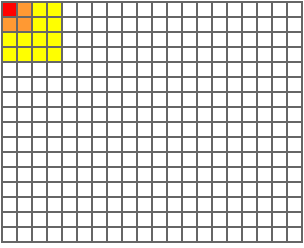
\includegraphics[width=\textwidth]{fig/4/ca-cfar-window-1.pdf}
        \caption{$(\gls{samplenumber}, \gls{chirpnumber}) = (0, 0)$}
    \end{subfigure}
    \hfill
    \begin{subfigure}[b]{0.3\textwidth}
        \centering
        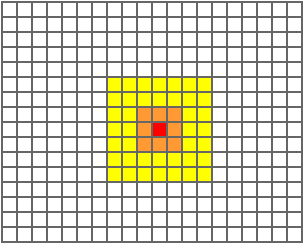
\includegraphics[width=\textwidth]{fig/4/ca-cfar-window-2.pdf}
        \caption{$(\gls{samplenumber}, \gls{chirpnumber}) = (\gls{numsamples}/2, \gls{numchirps}/2)$}
    \end{subfigure}
    \hfill
    \begin{subfigure}[b]{0.3\textwidth}
        \centering
        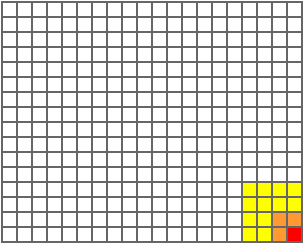
\includegraphics[width=\textwidth]{fig/4/ca-cfar-window-3.pdf}
        \caption{$(\gls{samplenumber}, \gls{chirpnumber}) = (\gls{numsamples}-1, \gls{numchirps}-1)$}
    \end{subfigure}
    \caption{
        The observation window, guard cells and test cell in the Cell Averaging Constant False Alarm Rate algorithm.
        The test cell is highlighted in red, guard cells in orange, and noise estimation window in yellow.
        In all cases, the noise estimation window has dimensions $7 \times 7$ and the guard window has dimensions $3 \times 3$.
    }
    \label{fig:ca-cfar-window}
\end{figure}

In a multitarget situation, the average noise power estimate of \gls{ca}-\gls{cfar} is no longer a good estimate,
as it is skewed from targets appearing inside the noise estimating window.
The average noise level is thus estimated too high and weak targets are "masked" by nearby strong targets,
which causes type \rom{2} errors (\gls{null-hypothesis} is erroneously accepted).
The \gls{os}-\gls{cfar} algorithm may be deployed in multi-target situations to achieve better detection performance.~\cite{nato-radar-topics}

In the \gls{os}-\gls{cfar} algorithm, the powers of the cells inside the observation window are sorted in smallest-first order.
The $\gls{targetnumber}$:th element is then picked from the sorted array and used as the average noise power estimate.
Given the observation window has dimensions $\gls{cfar-wnd-height} \times \gls{cfar-wnd-width}$, based on the work of Rohling, a reasonable value for is $\gls{targetnumber} = \frac{3}{4}\gls{cfar-wnd-height}\gls{cfar-wnd-width}$.
In the \gls{os}-\gls{cfar} algorithm, the guard cells are omitted.
\cite{radar-cfar-thresholding-in-clitter-and-multiple-target-situations}
The figure \ref{fig:cfar-plots} illustrates the results of applying the \gls{ca}- and \gls{os}-\gls{cfar} algorithms
on the range-velocity and range-angle spectra. The range-angle spectrum is calculated via the \gls{2d-music} algorithm whereas the range-velocity
spectrum is calculated via \gls{2d-fft}.
It is apparent from figure \ref{fig:os-cfar-music} that the exponentially distributed noise power assumption may not be good for the \gls{2d-music} spectrum.
The effects of masking in the \gls{ca}-\gls{cfar} algorithm can be seen by comparing figures \ref{fig:ca-cfar-fft} and \ref{fig:os-cfar-fft}.

\begin{figure}[H]
    \centering
    \begin{subfigure}{0.49\textwidth}
        \centering
        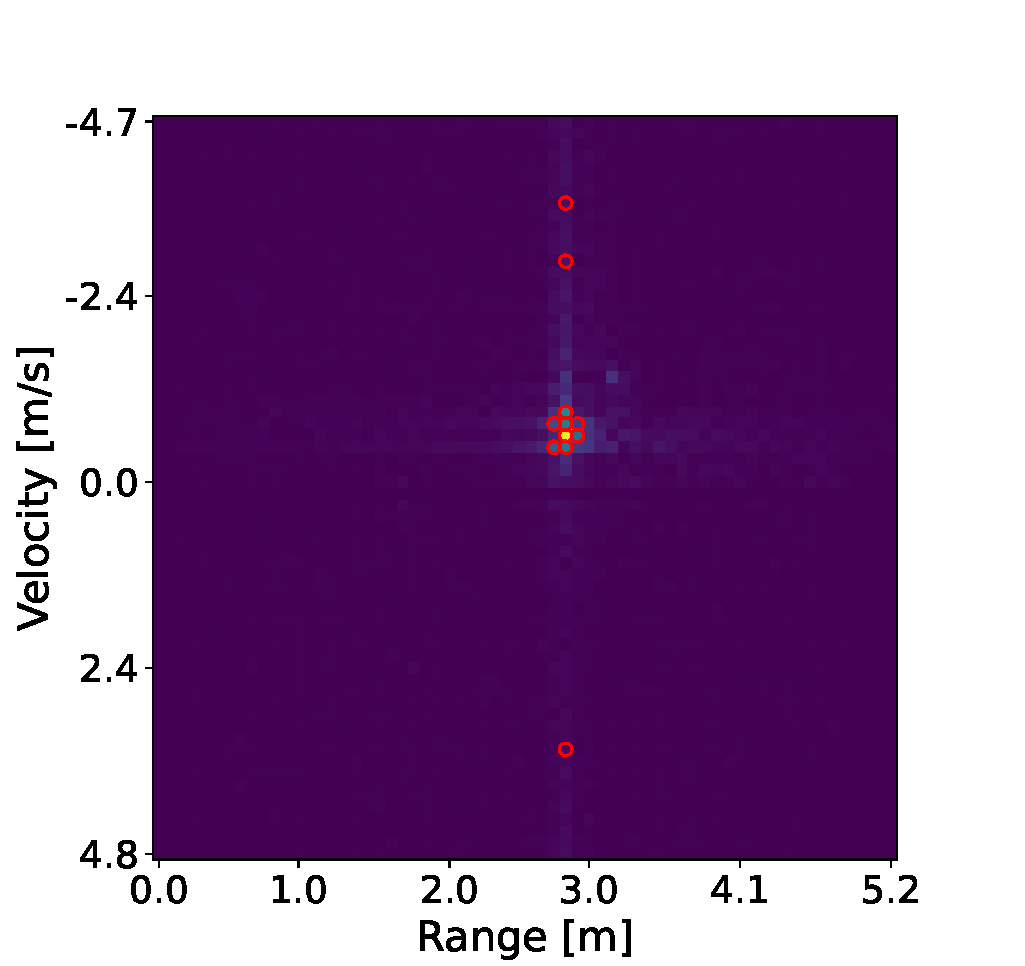
\includegraphics[width=\textwidth]{fig/4/ca-cfar-fft.pdf}
        \caption{CA-CFAR applied on range-velocity spectrum calculated via FFT.}
        \label{fig:ca-cfar-fft}
    \end{subfigure}
    \hfill
    \begin{subfigure}{0.49\textwidth}
        \centering
        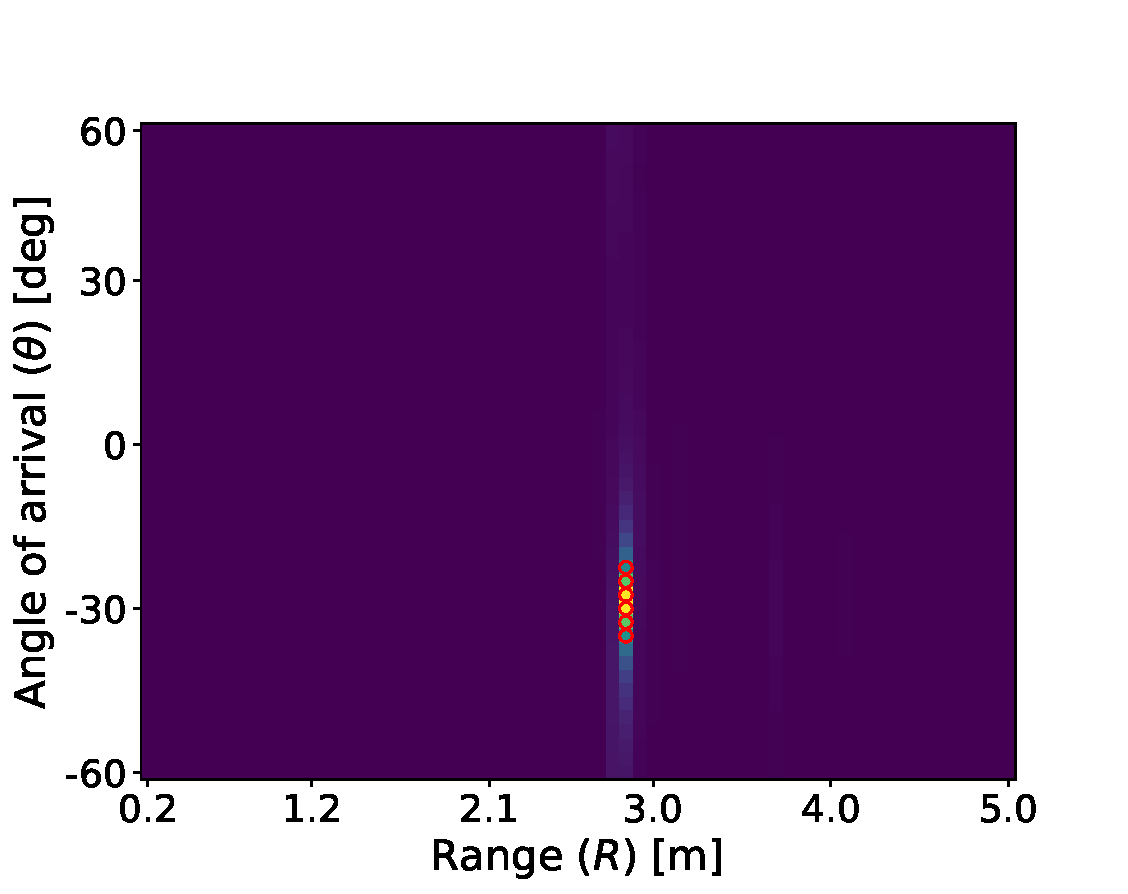
\includegraphics[width=\textwidth]{fig/4/ca-cfar-music.pdf}
        \caption{CA-CFAR applied on range-angle spectrum calculated via 2D-MUSIC.}
        \label{fig:ca-cfar-music}
    \end{subfigure}
    \vskip\baselineskip
    \begin{subfigure}{0.49\textwidth}
        \centering
        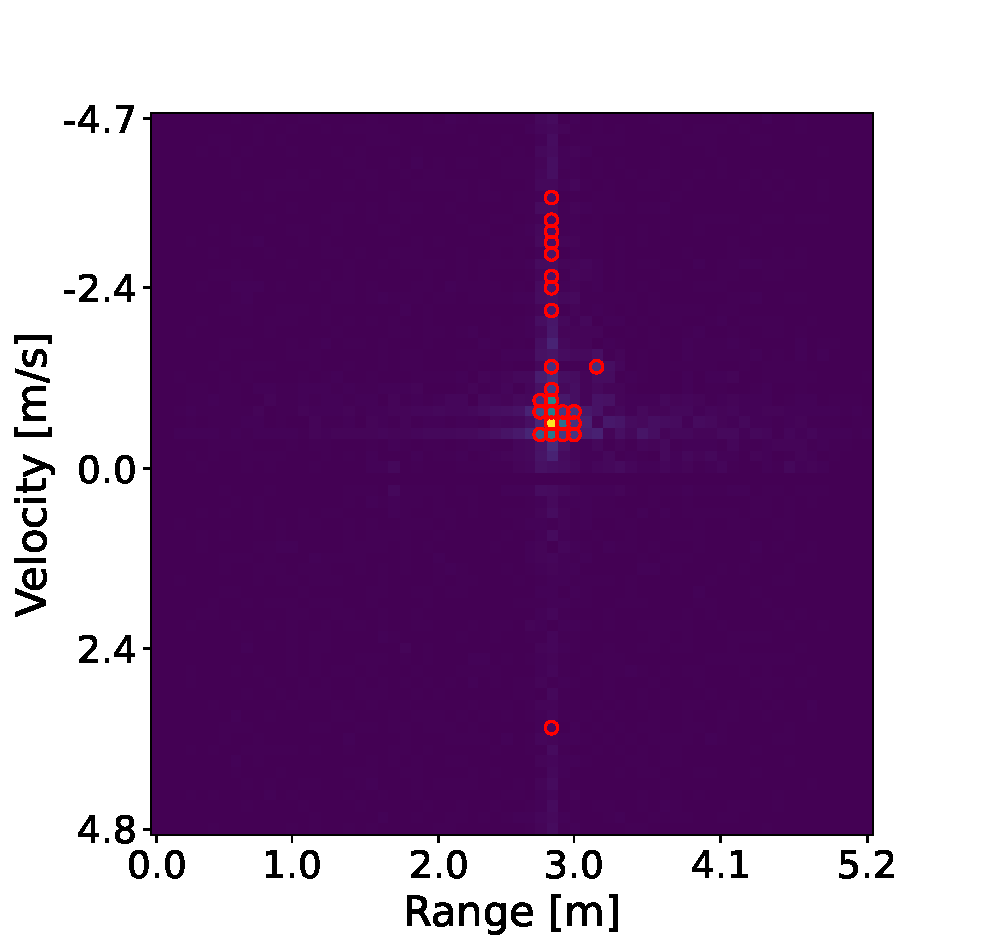
\includegraphics[width=\textwidth]{fig/4/os-cfar-fft.pdf}
        \caption{OS-CFAR applied on range-velocity spectrum calculated via FFT.}
        \label{fig:os-cfar-fft}
    \end{subfigure}
    \hfill
    \begin{subfigure}{0.49\textwidth}
        \centering
        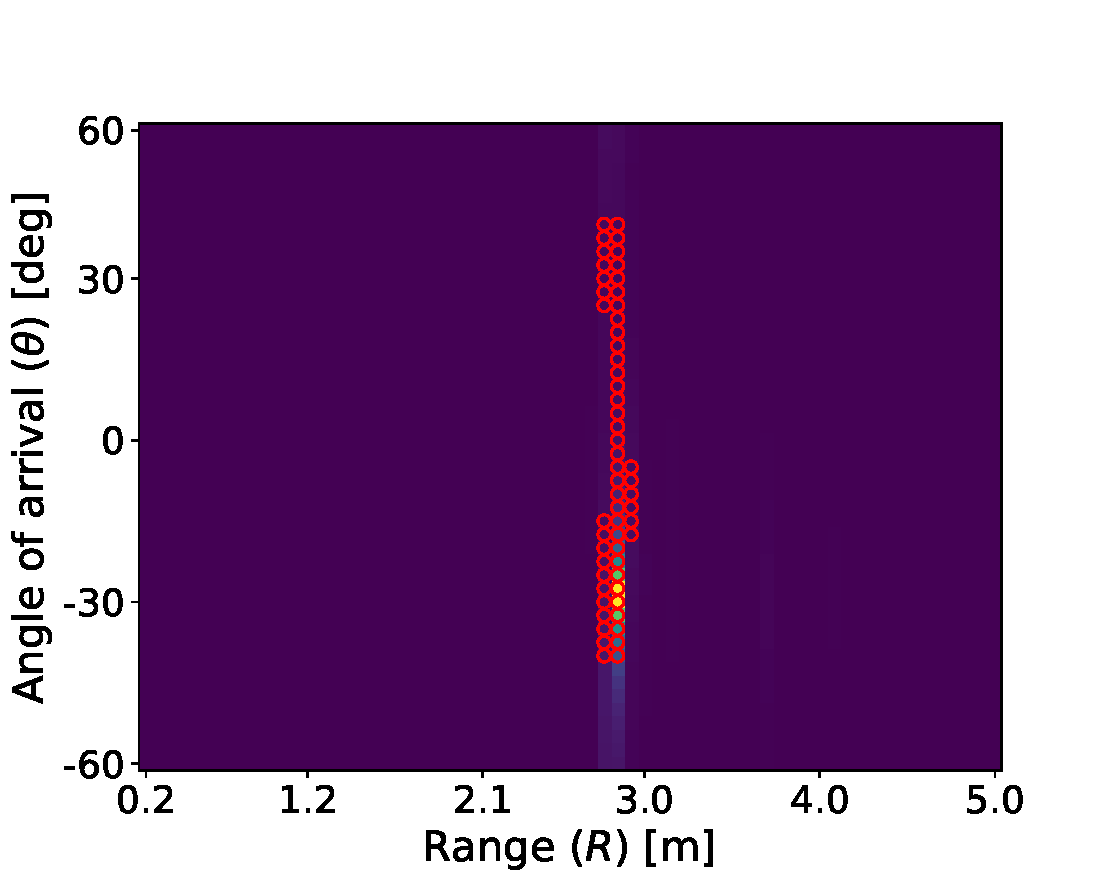
\includegraphics[width=\textwidth]{fig/4/os-cfar-music.pdf}
        \caption{OS-CFAR applied on range-angle spectrum calculated via 2D-MUSIC.}
        \label{fig:os-cfar-music}
    \end{subfigure}
    \caption{
        The Cell Averaging and Ordered Statistic Constant False Alarm Rate algorithms applied on the range-velocity and range-angle spectra.
        The figures are scaled show the amplitude of the spectrum rather than power.
    }
    \label{fig:cfar-plots}
\end{figure}

In addition to the basic \gls{ca}- and \gls{os}-\gls{cfar} algorithms, multiple variations and combinations of the two have been developed over the years.
The \gls{ca}- and \gls{os}-\gls{cfar} still serve as the basis for most of the variations.
The variations typically consider different computational complexity, noise distribution,
target amplitude statistics, and multiple target situations.~\cite{nato-radar-topics}

After target detection, target tracking algorithms may be used to track the same target between multiple frames.
With target tracking, the track of a single target may be recorded and predicted
and the appearance of new targets and the disappearance of old targets may be detected.
Additionally, when the velocity spectrum of a single target can be recorded through multiple frames,
this information can be used for \gls{har}.

Target tracking can be split into two parts: track filtering and measurement-to-track association.
The first part considers predicting the possible target tracks to determine the possible locations for a target in upcoming frames.
The latter part considers assigning measurements (detected targets) to predicted paths.
For track filtering, Kalman filtering is a popular choice.
For measurement-to-track association, nearest-neighbour filtering or probabilistic models are commonly used.~\cite{modern-radar-1}

\section{Depth camera record}   
\label{sec:depth-file}
The depth camera record is stored in the \texttt{depth.raw} file.
The recording program produces two bytes of output per pixel.
The output represents the measured distance at the pixel in millimeters as a 16-bit integer number (short int).
The frame resolution and frame rate are stored in the \texttt{metadata.yaml} file.
Table \ref{tab:depth-metadata} documents the metadata fields recorded under the \texttt{camera.depth} section in \texttt{metadata.yaml} file.
\begin{table}
    \begin{tabular}{l l}
        \toprule
        \textbf{Key} & \textbf{Meaning} \\
        \midrule
        framerate & Number of recorded frames per second, decimal number \\
        resolution & Resolution of the stored frames, string representation of a list: \texttt{'[\gls{width},\gls{height}]'} \\
        \bottomrule
    \end{tabular}
    \caption{Metadata fields for the depth camera.}
    \label{tab:depth-metadata}
\end{table}

Given the resolution is $\gls{height} \times \gls{width}$ (height $\times$ width) and the recorded data is represented by \gls{data},
where each element is two bytes long, the index of the $i$:th pixel of the $\gls{framenumber}$:th frame $\gls{frame-z-vector}(i)$ can be calculated using equation \ref{eq:depth-pixel}.

\begin{equation}
    \label{eq:depth-pixel}
    \forall i \in \left[ 0, \gls{width}\gls{height}-1 \right] \land \gls{framenumber} \in \left[ 0, \frac{| \gls{data} |}{\gls{width}\gls{height}}-1 \right] : \gls{frame-z-vector}(i) = \gls{data}(\gls{width}\gls{height}\gls{framenumber}+i)
\end{equation}

The frame \gls{frame-z-vector} can then be rearranged as a matrix \gls{frame-z},
which represents the pixels of the image in such a way that the origin is in the upper left corner.
The pixel in coordinates $(\gls{pixelrow},\gls{pixelcol})$ in the frame \gls{frame-z} is given by the equation \ref{eq:pixel-in-frame-depth}.

\begin{equation}
    \label{eq:pixel-in-frame-depth}
    \forall h \in [0, \gls{height}-1] \land w \in [0, \gls{width}-1] : \gls{frame-z}(h,w) = \gls{frame-z-vector}(h\gls{width}+w)
\end{equation}

Given the \gls{fov} of the sensor is $\gls{fovmax-az} \times \gls{fovmax-alt}$ in the azimuth and altitude dimensions respectively,
the \gls{fov} of each subpixel is $\frac{\gls{fovmax-az}}{\gls{width}} \times \frac{\gls{fovmax-alt}}{\gls{height}}$.
Given the angle is measured from the upper-left corner of a pixel and origin is in the center pixel,
the range (in the $\gls{framenumber}$:th frame) $\gls{range}_{\gls{framenumber}}$ measured at angle $(\gls{angle-alt}, \gls{angle-az})$ 
is given by equation \ref{eq:depth-range-angle}.
The term $1 \div 1000$ converts the measured range from millimeters to meters.

\begin{equation}
    \label{eq:depth-range-angle}
    \forall \gls{angle-alt} \in \left[ -\frac{\gls{fovmax-alt}}{2}, \frac{\gls{fovmax-alt}}{2} \right] \land \gls{angle-az} \in \left[ -\frac{\gls{fovmax-az}}{2}, \frac{\gls{fovmax-az}}{2} \right] :
    R_z(\gls{angle-alt}, \gls{angle-az}) =
    \frac{1}{1000} 
    \vec{F}_z \left(
        \left\lfloor \frac{\gls{height}}{2} + \frac{\gls{height}\gls{angle-alt}}{\gls{fovmax-alt}} \right\rfloor ,
        \left\lfloor \frac{\gls{width}}{2} + \frac{\gls{width}\gls{angle-az}}{\gls{fovmax-az}} \right\rfloor
    \right)
\end{equation}

\begin{figure}[H]
    \centering
    \begin{subfigure}[t]{0.49\textwidth}
        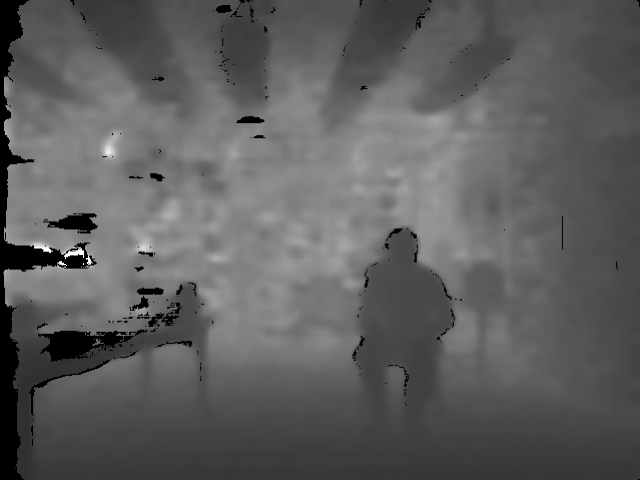
\includegraphics[width=\textwidth]{fig/4/depth-image.png}
        \caption{An example depth image.}
        \label{fig:depth-camera-frame}
    \end{subfigure}
    \hfill
    \begin{subfigure}[t]{0.49\textwidth}
        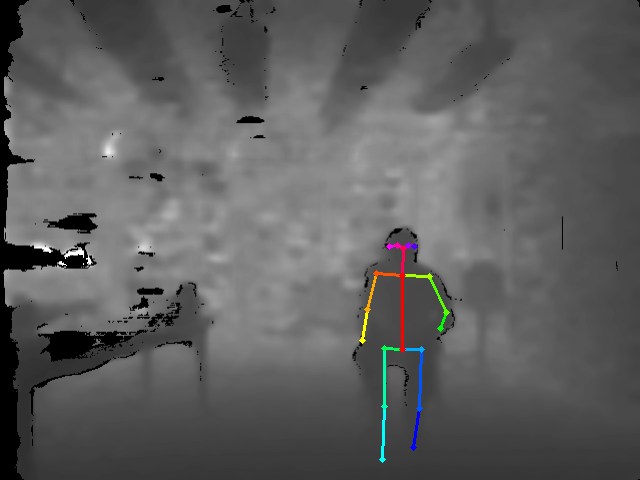
\includegraphics[width=\textwidth]{fig/4/depth-image-skeleton.png}
        \caption{Joint position information extracted from the depth image (PNG) using OpenPose~\cite{openpose}.}
        \label{fig:depth-camera-frame-skeleton}
    \end{subfigure}
    \caption{Depth image extracted from the \texttt{depth.raw} file.}
\end{figure}

Appendix \ref{app:image-parsing} shows an example of parsing the depth camera frames from the recorded data.
An example of a resulting image is presented in Figure \ref{fig:depth-camera-frame}.
Machine learning models may be used to extract e.g. posture information from the depth images.
Example models include TexMesh~\cite{tex-mesh}, A2J~\cite{a2j}, and DoubleFusion~\cite{double-fusion}.
Figure \ref{fig:depth-camera-frame-skeleton} shows an example of an image where the joint positions have been estimated using
OpenPose~\cite{openpose} from the depth image that has been exported to PNG format and rendered to the image.

\section{RGB camera record}
\label{sec:rgb-file}
The RGB camera record is stored in the \texttt{rgb.raw} file.
The recording program produces three bytes of output per pixel. 
The bytes correspond to the red, green and blue values of the pixel,
such that the first byte tells the red value,
second byte tells the green value and the third byte tells the blue value.
Each byte represents an unsigned 8-bit integer.
The frame rate and resolution of the recording are stored in the \texttt{metadata.yaml} file
under the \texttt{camera.rgb} section.
Table \ref{tab:rgb-metadata} documents the metadata fields recorded for the RGB camera.

\begin{table}
    \begin{tabular}{l l}
        \toprule
        \textbf{Key} & \textbf{Meaning} \\
        \midrule
        framerate & Number of recorded frames per second, decimal number \\
        resolution & Resolution of the stored frames, string representation of a list: \texttt{'[\gls{width},\gls{height}]'} \\
        \bottomrule
    \end{tabular}
    \caption{Metadata fields for the RBG camera.}
    \label{tab:rgb-metadata}
\end{table}

Denoting the vector of bytes stored in the file as \gls{bytes},
the data may be organized in pixels such that the $i$:th pixel $\gls{pixels}(i)$ is given by equation \ref{eq:rgb-pixels}.
When the pixels have been parsed, given the resolution of the recording is $\gls{height} \times \gls{width}$ (height $\times$ width),
the \gls{framenumber}:th frame, denoted as \gls{frame-z} can be parsed based on equation \ref{eq:rgb-pixels-to-frames}.

\begin{align}
    \label{eq:rgb-pixels}
    &\forall i \in \left[ 0, \frac{ | \gls{bytes} | }{3} \right] : \gls{pixels}(i) = \begin{bmatrix} \gls{bytes}(3i) & \gls{bytes}(3i+1) & \gls{bytes}(3i+2) \end{bmatrix}^{\gls{transpose}}
    \\
    \label{eq:rgb-pixels-to-frames}
    &\forall \gls{framenumber} \in \left[ 0, \frac{|\gls{pixels}|}{\gls{height}\gls{width}} \right] : \gls{frame-z}(\gls{pixelrow}, \gls{pixelcol}) = \gls{pixels}(\gls{framenumber}\gls{height}\gls{width} + \gls{pixelrow}\gls{width} + \gls{pixelcol})
\end{align}

Appendix \ref{app:image-parsing} shows an example of parsing the RGB camera frames from the recorded data.
An example of a resulting image is presented in Figure \ref{fig:rgb-camera-frame}.
Machine learning models may be used to e.g. extract posture information or detect items from the RGB images.
Some example models are OpenPose~\cite{openpose}, VNect~\cite{vnect}, and MixSTE~\cite{mixste}.
Figure \ref{fig:rgb-camera-frame-skeleton} shows an example of an image
where the joint positions have been estimated using OpenPose~\cite{openpose}.

\begin{figure}[H]
    \centering
    \begin{subfigure}[t]{0.49\textwidth}
        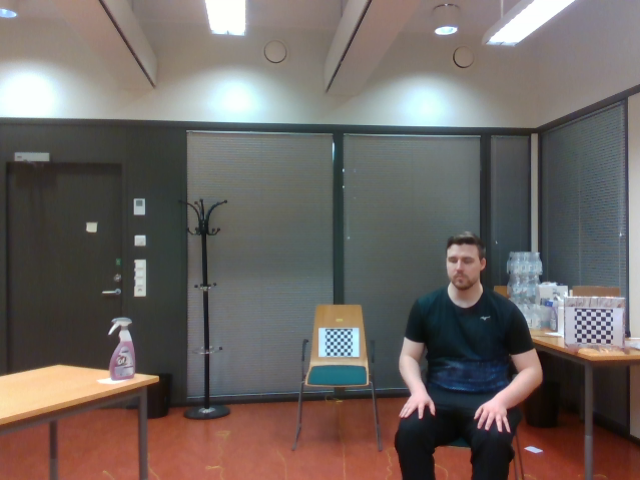
\includegraphics[width=\textwidth]{fig/4/rgb-image.png}
        \caption{An example RGB image.}
        \label{fig:rgb-camera-frame}
    \end{subfigure}
    \hfill
    \begin{subfigure}[t]{0.49\textwidth}
        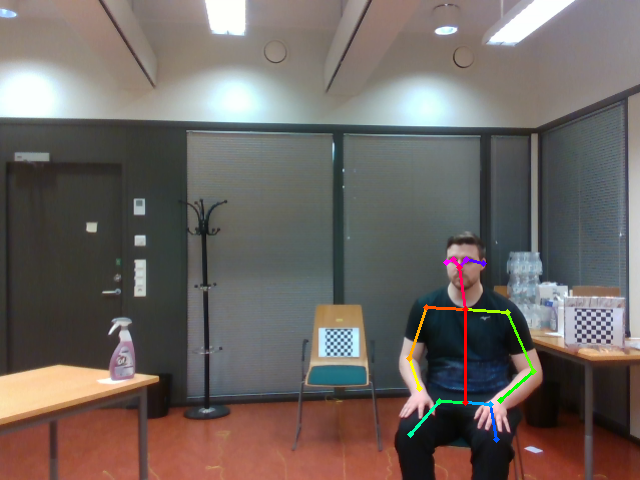
\includegraphics[width=\textwidth]{fig/4/rgb-image-skeleton.png}
        \caption{Joint position information extracted from the RGB using OpenPose\cite{openpose}.}
        \label{fig:rgb-camera-frame-skeleton}
    \end{subfigure}
    \caption{RGB image extracted from the \texttt{rgb.raw} file.}
\end{figure}

\section{Microphone samples}
\label{sec:audio-file}
The microphone record is stored in the \texttt{audio.wav} file. 
The file contains 16 audio channels and the sampling rate is stored in the \texttt{metadata.yaml} file.
The sampling rate is also stored as metadata in the WAV file.
Table \ref{tab:mic-metadata} documents the metadata recorded for the audio file in the \texttt{metadata.yaml} file in the \texttt{audio} section.

\begin{table}[H]
    \centering
    \begin{tabular}{l l}
        \toprule
        \textbf{Key} & \textbf{Meaning} \\
        \midrule
        samplerate & The sampling frequency for the microphone recording, integer number. \\
        \bottomrule
    \end{tabular}
    \caption{Metadata recorded for the \texttt{audio.wav} file.}
    \label{tab:mic-metadata}
\end{table}

Figure \ref{fig:mic-channels} shows the positions of the microphones in the used MiniDSP UMA-16 microphone.
The microphone numbers correspond to the audio channel numbers such that MIC1 is channel 0, MIC2 is channel 1, etc.
Each sample in the data is represented by a 32-bit floating-point number.
The samples are real-valued.
Appendix \ref{app:mic-parsing} shows an example of reading the audio file with Python using the Soundfile~\cite{python-soundfile} library.

\begin{figure}
    \centering
    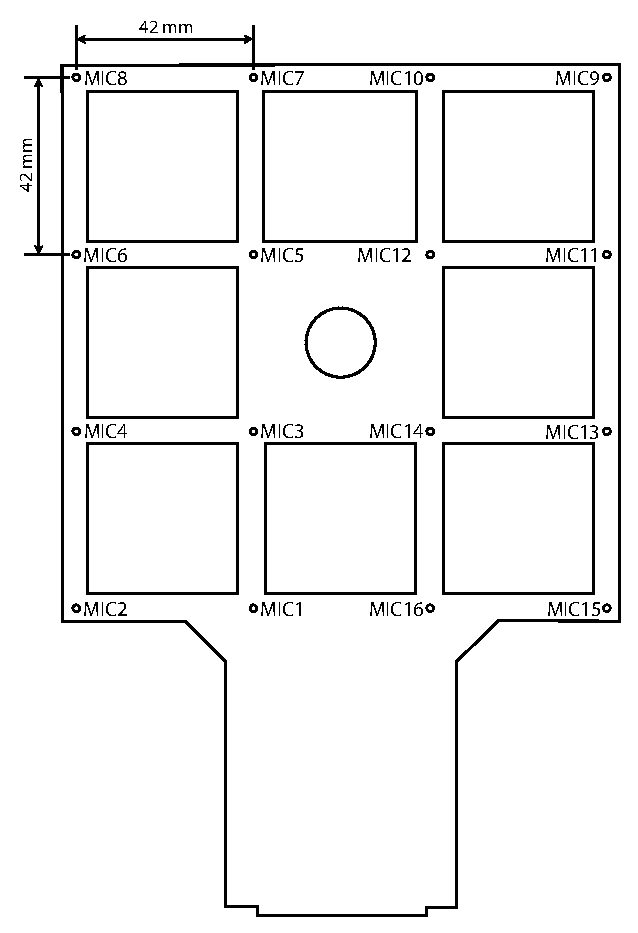
\includegraphics[width=0.67\textwidth]{fig/4/microphone-channels.eps}
    \caption{Channels of the MiniDSP UMA-16 microphone~\cite{minidsp-spec}.}
    \label{fig:mic-channels}
\end{figure}



\chapter{System evaluation}
\label{ch:5-evaluation}
In Section \ref{sec:2-requirements}, requirements for the data recording system were defined.
The quality of the system is evaluated based on the defined criteria.
Additionally, the extensibility and stability of the software are considered.

\section{Time synchronization of data}
The criterion for data synchronization was defined in \ref{sec:2-requirements}.
The frame number \gls{framenumber} that corresponds to a moment in time \gls{time} is given by the equation $\gls{framenumber} = \lfloor \gls{framerate} \gls{time} \rfloor$,
where \gls{framerate} is the frame rate (equation \ref{eq:time-to-sample}).
This holds true for any of the data sources.
Thus, if a frame corresponding to the same point in time is extracted from each data source,
high correlation should be seen between the frames.

In this case, evaluating the data synchronization is done
simply by calculating the range-angle spectrum from the radar frame and drawing it next to the RGB and \gls{ir} frames.
Because the RGB and Depth video are coming from the same sensor, they are guaranteed to be time-synchronized.
The drawn frames should look like they correspond to the same moment in time.

The audio sensor is omitted from this evaluation.
For audio-to-radar synchronization the angle of arrival of a single tone could be estimated from the audio signal.
Given the source for the tone is a radar target, the sound and radar angle-power spectrum could be observed
to see if the direction of arrival is correlated between the sensors.
For audio-to-video synchronization, a video could be recorded of a person starting a tone generator.
If the tone then appears in the audio signal at the same moment when the person starts the tone generator,
it could be concluded that the sound and audio recordings are synchronized.

\begin{figure}
    \centering
    \begin{subfigure}[t]{0.3\textwidth}
    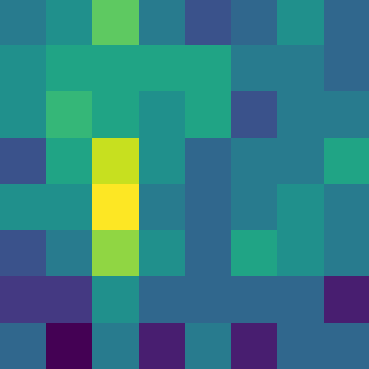
\includegraphics[width=\textwidth]{fig/5/ir_t_7.0.png}
        \caption{IR frame}
    \end{subfigure}
    \hfill
    \begin{subfigure}[t]{0.3\textwidth}
        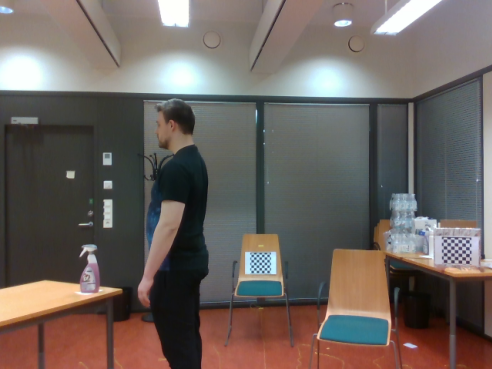
\includegraphics[width=\textwidth]{fig/5/rgb_t_7.0.png}
        \caption{RGB frame}
    \end{subfigure}
    \hfill
    \begin{subfigure}[t]{0.3\textwidth}
        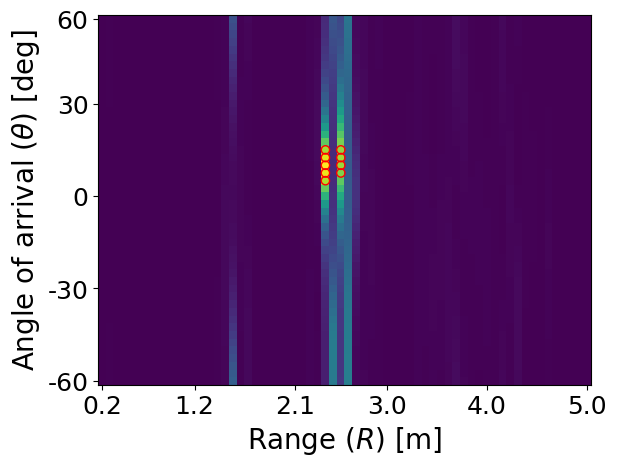
\includegraphics[width=\textwidth]{fig/5/radar_t_7.0.png}
        \caption{Radar angle-range spectrum}
    \end{subfigure}
    \caption{IR, RGB and radar frames, $\gls{time} = 7.0$.}
    \label{fig:5-frames-1}
\end{figure}

\begin{figure}
    \centering
    \begin{subfigure}[t]{0.3\textwidth}
        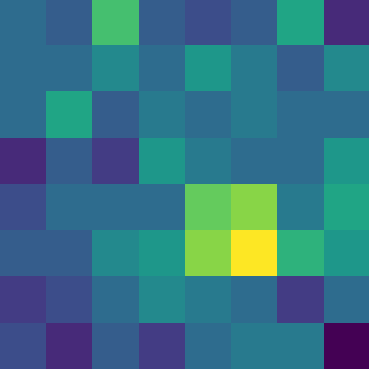
\includegraphics[width=\textwidth]{fig/5/ir_t_24.0.png}
        \caption{IR frame}
    \end{subfigure}
    \hfill
    \begin{subfigure}[t]{0.3\textwidth}
        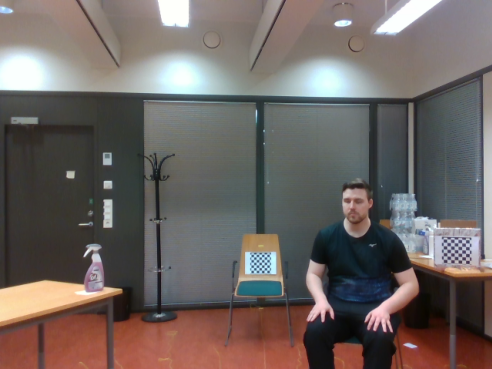
\includegraphics[width=\textwidth]{fig/5/rgb_t_24.0.png}
        \caption{RGB frame}
    \end{subfigure}
    \hfill
    \begin{subfigure}[t]{0.3\textwidth}
        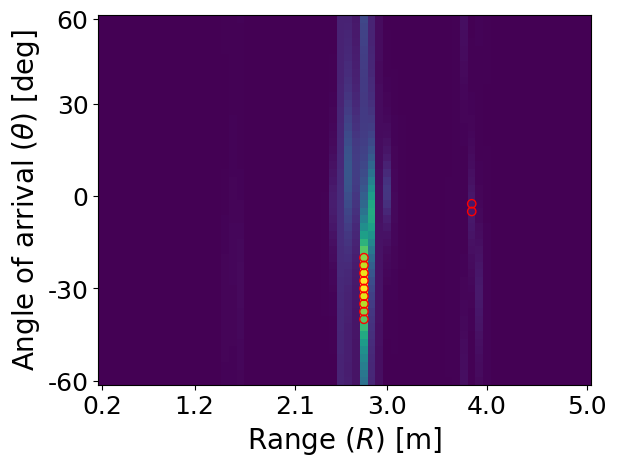
\includegraphics[width=\textwidth]{fig/5/radar_t_24.0.png}
        \caption{Radar angle-range spectrum}
    \end{subfigure}
    \caption{IR, RGB and radar frames, $\gls{time} = 24.0$.}
    \label{fig:5-frames-2}
\end{figure}

\begin{figure}
    \centering
    \begin{subfigure}[t]{0.3\textwidth}
        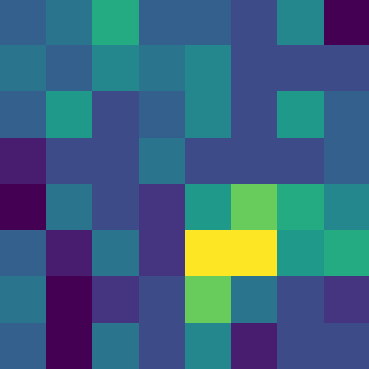
\includegraphics[width=\textwidth]{fig/5/ir_t_53.0.png}
    \end{subfigure}
    \hfill
    \begin{subfigure}[t]{0.3\textwidth}
        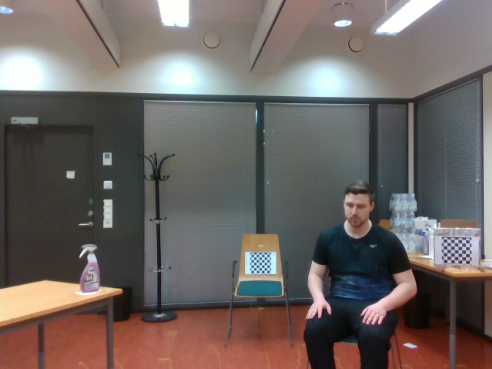
\includegraphics[width=\textwidth]{fig/5/rgb_t_53.0.png}
        \caption{RGB frame}
    \end{subfigure}
    \hfill
    \begin{subfigure}[t]{0.3\textwidth}
        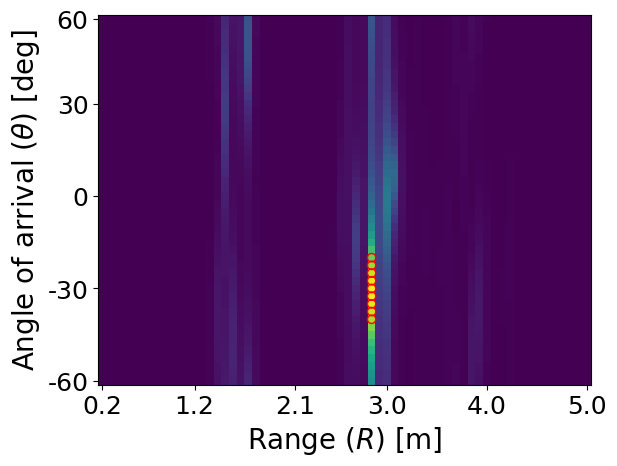
\includegraphics[width=\textwidth]{fig/5/radar_t_53.0.png}
        \caption{Radar angle-range spectrum}
    \end{subfigure}
    \caption{IR, RGB and radar frames, $\gls{time} = 53.0$.}
    \label{fig:5-frames-3}
\end{figure}

Figures \ref{fig:5-frames-1}--\ref{fig:5-frames-3} show the RGB, Radar (range-angle) and \gls{ir} frames
corresponding to different times. By looking at the frames, there seems to be high correlation between
the angle of the target, thus it can be concluded that the data is well synchronized.

\section{Data labelling}
The data can be semi-automatically labelled during testing.
Using this method, considerable effort must be made in planning the set of performed activities,
which makes the performance less natural.
Automatic activity recognition using i.e. RGB video based methods could also be used to produce the activity labels
in post-processing.
The generated labels could then be used as ground-truth information for the other sensors in machine learning algorithms.

The format of the activity labels is very simple and because the data sources are time synchronized and the frame/sampling rates are known,
it is easy to map the activities and data frames based on the time stamps and activity labels.
The data labelling can therefore be considered sufficient.

\section{Data structuring}
Each recording is stored in a single directory.
The software \gls{cli} provides a way to determine the name of the directory.
The directory names can thus be used as unique identifiers to the recordings,
and additional data such as person or room information can be mapped to the recordings using the directory names.

Under each directory, the files have consistent naming and the output from each sensor is stored in a separate file.
This makes it easy to pick and choose used sensors and minimizes the amount of data that has to be loaded into memory
for processing the output of a single sensor.

The data in the output files is unprocessed raw data from the sensors.
As a downside, lots of post-processing may be required but as an upside, no information is lost.
The structuring of the data, in the autor's opinion, is good.

\section{Metadata}
The recorded metadata considers only the sensor characteristics.
The metadata file is easy to parse programmatically as it follows the YAML syntax.
Sufficient parameter information is provided for processing the data.
Thus, the metadata can be considered sufficient.

\section{Extensibility of the system}
The system is easy to extend to include new sensors.
A recorder submodule must be written for each added sensor,
and the sensor must be added as a source to the recroded submodule.

The system was written using a very crude proceduric model.
Any well-established programming patterns were not followed.
This may have had negative effects on extensibility of the code.
Considering the module interfaces for the subprograms may have been worth considering.
Instead of passing constant strings as signals to control the program,
the signaling could have been abstracted to functions.

\section{Stability of the system}
In use, the system proved to be slightly instabile.
Sometimes after starting the software,
the recording never started as the system froze at some point of the initialization.
Power-cycling the radar device fixed the issue,
but this instability made the system much slower to use.

Effort should be made to fix the issue.
Since the issue was fixed by power-cycling the radar device,
the issue is likely related to not sending the correct commands to the radar device.
Because the issue did not occur every time,
it may also be related to parallelization.

\section{Radar data quality}
\label{sec:5-radar-spectrum-issues}
When processing the radar data, it was noticed that sometimes the range-angle spectrum
becomes extremely noisy. Figure \ref{fig:bad-radar-example} shows an example.
It may be worth investigating if using the two transmitter switching to increase the virtual number of receivers would alleviate this issue.

\begin{figure}[h]
    \centering
    \begin{subfigure}[t]{0.49\textwidth}
        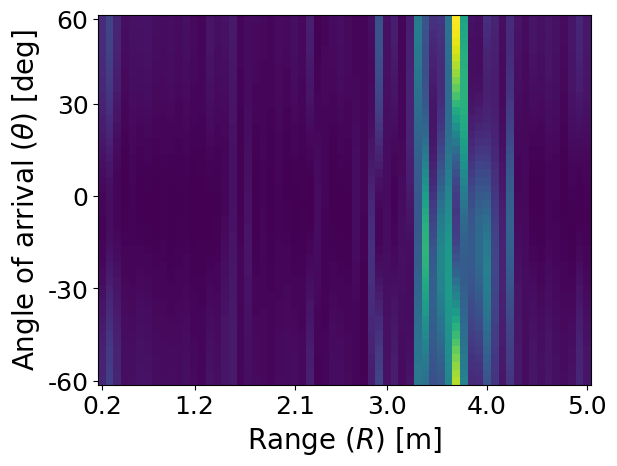
\includegraphics[width=\textwidth]{fig/5/bad-spectrum-example-radar.png}
        \caption{Radar angle-range spectrum.}
    \end{subfigure}
    \hfill
    \begin{subfigure}[t]{0.49\textwidth}
        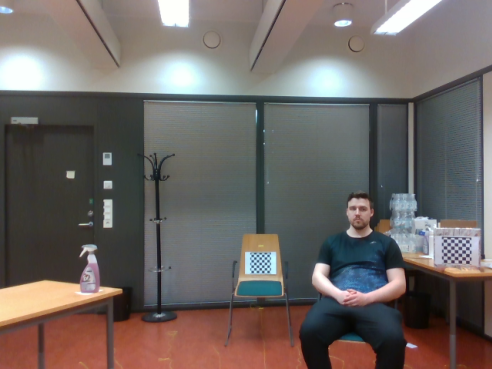
\includegraphics[width=\textwidth]{fig/5/bad-spectrum-example-rgb.png}
        \caption{Corresponding RGB image.}
    \end{subfigure}
    \caption{Example of a very noisy radar range-angle spectrum.}
    \label{fig:bad-radar-example}
\end{figure}

\chapter{Conclusion}
\label{ch:6-conclusion}
As the product of this thesis,
a multimodal sensor data recording system was produced.
The implementation of the system was discussed,
the produced data formats were documented and data processing examples were given to prove the documentation is truthful.
Additionally, the quality of the system was assessed.

The system is capable of recording five different modalities of data:
$4 \times 4$ acoustic, RGB video, depth video, $8 \times 8$ infrared video, and mmWave radar signal.
The system is very portable as the sensors can be mounted on a single bracket that attaches to a camera tri-pod.
Only a sufficient power source and a computer equipped with an \gls{ssd} drive are required.
Wearable sensors were omitted from the system due to being cumbersome.
Proximity sensors, such as magnetic switches, pressure plates, electrostatic sensors, etc. labour-intensive sensors were also omitted.

The system was designed to be parallel to maximize the data throughput.
Each sensor has its own recorder subprocess that is controlled by a single main process.
The subprograms are implemented as modules.
The system can be extended to include additional sensors by writing a recording module for the sensor,
and starting it from the main process.

The recorded data from the different sensors is synchronized in time.
This means, that given a point in time, a corresponding frame can be easily extracted from any of the sensor outputs.
In addition, the program provides a way to attach activity labels to the data during recording.
The activity labels are stored in a separate file and the file format is very simple.
It is also possible to apply the activity labels after recording.
Manual labelling can be used for ultimate accuracy, or well-established activity recognition models can be used to detect actions form the RGB video.
The labels can then be used as ground-truth information to train a machine learning model to recognize activities from the data produced by the other sensors.

The output from each sensor is stored in separate files and each recording is stored in a separate directory.
Based on the output formats documented in Chapter \ref{ch:4-files-and-post},
the data may be parsed into other formats, such as the popular \texttt{.mat} format used by MATLAB.
Additionally, post-processing may be performed on the data to make it more suitable for machine learning.
Most importantly, the range-angle and range-velocity spectra of the radar may be calculated
using the algorithms presented in Sections \ref{sec:range-angle} and \ref{sec:doppler-spectrum}.

While the system fulfilled the requirements set for in in Chapter \ref{ch:2-premise},
some instability was detected when using it,
which makes the system unusable for carrying out a large-scale data recording campaign.
For small-scale campaigns, the system is satisfactory.

Sometimes, after starting, the system freezes.
It is unclear whether this is caused by problems in the parallel design,
or whether it is caused by the radar sensor.
Power-cycling the radar sensor and restarting the program fixed the issue with a high likelihood, though,
which suggests that the problem may be caused by the radar.
It should be looked into, if there is some further configuration that can be done to the radar device to increase its stability.

Additionally, the range-angle spectrum was extremely noisy in some frames.
This issue was discussed in Section \ref{sec:5-radar-spectrum-issues}.
The cause of the noisiness should be investigated.
It should also be investigated if the issue can be alleviated by using the two-transmitter switching to increase the virtual number
of receivers from 4 to 8.
It is also possible that the used radar processing algorithms could be improved to produce a better range-angle estimate.

All in all, the implemented system serves a good basis.
Some further development must still be done,
but the system serves as a very good Proof of Concept.
When the stability issues have been fixed,
carrying out a larger-scale data collection campaign with the system should be feasible.

Even with small data sets, some preliminary research may be done with the system, especially considering transfer learning.
Machine learning models trained with other data sets can be evaluated on data sets recorded on this system to see how the performance carries over.
In addition, once the stability issues are fixed in the system,
the data can even be used for training machine learning models.
With the portable system, high quality data sets should be possible to collect,
which will enable high-performance human activity recognition using remote sensing in various environments.

%%%%% Bibliography/references.
\printbibliography[heading=bibintoc]

%%%%% Appendices.

\begin{appendices}

\chapter{Radar configuration file used during testing and development of the system}
\label{app:config}
\begin{lstlisting}
sensorStop
flushCfg
dfeDataOutputMode 1
channelCfg 15 7 0
adcCfg 2 1
adcbufCfg -1 0 1 1 1
profileCfg 0 60 219 7 40 0 0 100 1 64 3500 0 0 30
chirpCfg 0 0 0 0 0 0 0 2
frameCfg 0 0 64 0 33.333 1 0
lowPower 0 0
guiMonitor -1 0 0 0 0 0 0
cfarCfg -1 0 2 8 4 3 0 15 1
cfarCfg -1 1 0 8 4 4 1 15 1
multiObjBeamForming -1 1 0.5
clutterRemoval -1 0
calibDcRangeSig -1 0 -5 8 256
extendedMaxVelocity -1 0
bpmCfg -1 0 0 1
lvdsStreamCfg -1 0 0 0
compRangeBiasAndRxChanPhase 0.0 1 0 1 0 1 0 1 0 1 0 1 0 1 0 1...
                                           ... 0 1 0 1 0 1 0 1 0
measureRangeBiasAndRxChanPhase 0 1.5 0.2
CQRxSatMonitor 0 3 4 99 0
CQSigImgMonitor 0 63 4
analogMonitor 0 0
aoaFovCfg -1 -90 90 -90 90
cfarFovCfg -1 0 0 4.79
cfarFovCfg -1 1 -2.41 2.41
lvdsStreamCfg -1 0 1 0
\end{lstlisting}

\chapter{DCA1000EVM configuration commands}
\label{app:dca1000evm-commands}
This page is empty on purpose
\newpage

\section{RESET\_FPGA\_CMD\_CODE}
Reset FPGA
\subsection{Request}
\begin{table}[H]
    \centering
    \begin{tabular}{|
    >{\centering\arraybackslash}p{1.8cm}|
    >{\centering\arraybackslash}p{1.4cm}|
    >{\centering\arraybackslash}p{1.5cm}|
    >{\centering\arraybackslash}p{1.5cm}|
    >{\centering\arraybackslash}p{1cm}|
    >{\centering\arraybackslash}p{1cm}|
    >{\centering\arraybackslash}p{3.75cm}|
    }
        \hline
        Name & Data Type & Number of bytes & Default Value & Min Value & Max Value & Description \\
        \hline
        Header             & UINT16 & 2 & 0xA55A & - & - & 0xA55A always. Start bits of packet. \\ \hline
        Command code       & UINT16 & 2 & 0x01 & - & - & Command code \\ \hline
        Size               & UINT16 & 2 & 0 & - & - & Data size \\ \hline
        Footer             & UINT16 & 2 & 0xEEAA & - & - & 0xEEAA always. Stop bits of packet. \\
        \hline
    \end{tabular}
\end{table}

\subsection{Response}
\begin{table}[H]
    \centering
    \begin{tabular}{|
    >{\centering\arraybackslash}p{1.8cm}|
    >{\centering\arraybackslash}p{1.4cm}|
    >{\centering\arraybackslash}p{1.5cm}|
    >{\centering\arraybackslash}p{1.5cm}|
    >{\centering\arraybackslash}p{1cm}|
    >{\centering\arraybackslash}p{1cm}|
    >{\centering\arraybackslash}p{3.75cm}|
    }
        \hline
        Name & Data Type & Number of bytes & Default Value & Min Value & Max Value & Description \\
        \hline
        Header             & UINT16 & 2 & 0xA55A & - & - & 0xA55A always. Start bits of packet. \\ \hline
        Command code       & UINT16 & 2 & 0x01 & - & - & Command code \\ \hline
        Status             & UINT16 & 2 & 0 & 0 & 1 & \makecell{0 -- Success \\ 1 -- Failure } \\ \hline
        Footer             & UINT16 & 2 & 0xEEAA & - & - & 0xEEAA always. Stop bits of packet. \\
        \hline
    \end{tabular}
\end{table}

\newpage
\section{RESET\_AR\_DEV\_CMD\_CODE}
Reset RADAR EVM
\subsection{Request}
\begin{table}[H]
    \centering
    \begin{tabular}{|
    >{\centering\arraybackslash}p{1.8cm}|
    >{\centering\arraybackslash}p{1.4cm}|
    >{\centering\arraybackslash}p{1.5cm}|
    >{\centering\arraybackslash}p{1.5cm}|
    >{\centering\arraybackslash}p{1cm}|
    >{\centering\arraybackslash}p{1cm}|
    >{\centering\arraybackslash}p{3.75cm}|
    }
        \hline
        Name & Data Type & Number of bytes & Default Value & Min Value & Max Value & Description \\
        \hline
        Header             & UINT16 & 2 & 0xA55A & - & - & 0xA55A always. Start bits of packet. \\ \hline
        Command code       & UINT16 & 2 & 0x02 & - & - & Command code \\ \hline
        Size               & UINT16 & 2 & 0 & - & - & Data size \\ \hline
        Footer             & UINT16 & 2 & 0xEEAA & - & - & 0xEEAA always. Stop bits of packet. \\
        \hline
    \end{tabular}
\end{table}

\subsection{Response}
\begin{table}[H]
    \centering
    \begin{tabular}{|
    >{\centering\arraybackslash}p{1.8cm}|
    >{\centering\arraybackslash}p{1.4cm}|
    >{\centering\arraybackslash}p{1.5cm}|
    >{\centering\arraybackslash}p{1.5cm}|
    >{\centering\arraybackslash}p{1cm}|
    >{\centering\arraybackslash}p{1cm}|
    >{\centering\arraybackslash}p{3.75cm}|
    }
        \hline
        Name & Data Type & Number of bytes & Default Value & Min Value & Max Value & Description \\
        \hline
        Header             & UINT16 & 2 & 0xA55A & - & - & 0xA55A always. Start bits of packet. \\ \hline
        Command code       & UINT16 & 2 & 0x02 & - & - & Command code \\ \hline
        Status             & UINT16 & 2 & 0 & 0 & 1 & \makecell{0 -- Success \\ 1 -- Failure } \\ \hline
        Footer             & UINT16 & 2 & 0xEEAA & - & - & 0xEEAA always. Stop bits of packet. \\
        \hline
    \end{tabular}
\end{table}

\newpage
\section{CONFIG\_FPGA\_GEN\_CMD\_CODE}
\label{app:sec:config-fpga}
Configure FPGA
\subsection{Request}
\begin{table}[H]
    \centering
    \begin{tabular}{|
    >{\centering\arraybackslash}p{1.8cm}|
    >{\centering\arraybackslash}p{1.4cm}|
    >{\centering\arraybackslash}p{1.5cm}|
    >{\centering\arraybackslash}p{1.5cm}|
    >{\centering\arraybackslash}p{1cm}|
    >{\centering\arraybackslash}p{1cm}|
    >{\centering\arraybackslash}p{3.75cm}|
    }
        \hline
        Name & Data Type & Number of bytes & Default Value & Min Value & Max Value & Description \\
        \hline
        Header             & UINT16 & 2 & 0xA55A & - & - & 0xA55A always. Start bits of packet. \\ \hline
        Command code       & UINT16 & 2 & 0x03 & - & - & Command code \\ \hline
        Size               & UINT16 & 2 & 6 & - & - & Data size \\ \hline
        Data Logging Mode  & UINT8 & 1 & 1 & 1 & 2 & \makecell{1 -- Raw mode \\ 2 -- Multi mode} \\ \hline
        LVDS mode          & UINT8 & 1 & 1 & 1 & 2 & \makecell{1 -- 4lane \\ 2 -- 2lane} \\ \hline
        Data transfer mode & UINT8 & 1 & 1 & 1 & 2 & \makecell{1 -- LVDS capture \\ 2 -- DMM playback } \\\hline
        Data capture mode  & UINT8 & 1 & 2 & 1 & 2 & \makecell{1 -- SD card storage \\ 2 -- Ethernet stream } \\ \hline
        Data format mode   & UINT8 & 1 & 2 & 1 & 3 & \makecell{1 -- 12-bit \\ 2 -- 14-bit \\ 3 -- 16-bit } \\ \hline
        Timer              & UINT8 & 1 & 30 (0x1E) & 0x0 & 0xFF & Timer info in seconds \\ \hline
        Footer             & UINT16 & 2 & 0xEEAA & - & - & 0xEEAA always. Stop bits of packet. \\
        \hline
    \end{tabular}
\end{table}

\subsection{Response}
\begin{table}[H]
    \centering
    \begin{tabular}{|
    >{\centering\arraybackslash}p{1.8cm}|
    >{\centering\arraybackslash}p{1.4cm}|
    >{\centering\arraybackslash}p{1.5cm}|
    >{\centering\arraybackslash}p{1.5cm}|
    >{\centering\arraybackslash}p{1cm}|
    >{\centering\arraybackslash}p{1cm}|
    >{\centering\arraybackslash}p{3.75cm}|
    }
        \hline
        Name & Data Type & Number of bytes & Default Value & Min Value & Max Value & Description \\
        \hline
        Header             & UINT16 & 2 & 0xA55A & - & - & 0xA55A always. Start bits of packet. \\ \hline
        Command code       & UINT16 & 2 & 0x03 & - & - & Command code \\ \hline
        Status             & UINT16 & 2 & 0 & 0 & 1 & \makecell{0 -- Success \\ 1 -- Failure } \\ \hline
        Footer             & UINT16 & 2 & 0xEEAA & - & - & 0xEEAA always. Stop bits of packet. \\
        \hline
    \end{tabular}
\end{table}

\newpage
\section{CONFIG\_EEPROM\_CMD\_CODE}
Configure EEPROM

\subsection{Request}
\begin{table}[H]
    \centering
    \begin{tabular}{|
    >{\centering\arraybackslash}p{1.8cm}|
    >{\centering\arraybackslash}p{1.4cm}|
    >{\centering\arraybackslash}p{1.5cm}|
    >{\centering\arraybackslash}p{2.75cm}|
    >{\centering\arraybackslash}p{1cm}|
    >{\centering\arraybackslash}p{1.5cm}|
    >{\centering\arraybackslash}p{2cm}|
    }
        \hline
        Name & Data Type & Number of bytes & Default Value & Min Value & Max Value & Description \\
        \hline
        Header             & UINT16 & 2 & 0xA55A & - & - & 0xA55A always. Start bits of packet. \\ \hline
        Command code       & UINT16 & 2 & 0x04 & - & - & Command code \\ \hline
        Size               & UINT16 & 2 & 6 & - & - & Data size \\ \hline
        System IP address  & UINT8  & 4 & 192.168.33.30     & 0x0 & 0xFF   & IP address \\\hline
        FPGA IP address    & UINT8  & 4 & 192.168.33.180    & 0x0 & 0xFF   & IP address \\ \hline
        FPGA MAC address   & UINT8  & 6 & 12-34-56-78-90-12 & 0x0 & 0xFF   & MAC address \\ \hline
        \makecell{Configu-\\ration port} & UINT16 & 2 & 4096 & 0x1 & 0xFFFF & Config Port number \\ \hline
        Data port          & UINT16 & 2 & 4098              & 0x1 & 0xFFFF & Data Port number \\ \hline
        Footer             & UINT16 & 2 & 0xEEAA & - & - & 0xEEAA always. Stop bits of packet. \\
        \hline
    \end{tabular}
\end{table}

\subsection{Response}
\begin{table}[H]
    \centering
    \begin{tabular}{|
    >{\centering\arraybackslash}p{1.8cm}|
    >{\centering\arraybackslash}p{1.4cm}|
    >{\centering\arraybackslash}p{1.5cm}|
    >{\centering\arraybackslash}p{1.5cm}|
    >{\centering\arraybackslash}p{1cm}|
    >{\centering\arraybackslash}p{1cm}|
    >{\centering\arraybackslash}p{3.75cm}|
    }
        \hline
        Name & Data Type & Number of bytes & Default Value & Min Value & Max Value & Description \\
        \hline
        Header             & UINT16 & 2 & 0xA55A & - & - & 0xA55A always. Start bits of packet. \\ \hline
        Command code       & UINT16 & 2 & 0x04 & - & - & Command code \\ \hline
        Status             & UINT16 & 2 & 0 & 0 & 1 & \makecell{0 -- Success \\ 1 -- Failure } \\ \hline
        Footer             & UINT16 & 2 & 0xEEAA & - & - & 0xEEAA always. Stop bits of packet. \\
        \hline
    \end{tabular}
\end{table}

\newpage
\section{RECORD\_START\_CMD\_CODE}
\label{app:sec:start-record}
Start record
\subsection{Request}
\begin{table}[H]
    \centering
    \begin{tabular}{|
    >{\centering\arraybackslash}p{1.8cm}|
    >{\centering\arraybackslash}p{1.4cm}|
    >{\centering\arraybackslash}p{1.5cm}|
    >{\centering\arraybackslash}p{1.5cm}|
    >{\centering\arraybackslash}p{1cm}|
    >{\centering\arraybackslash}p{1cm}|
    >{\centering\arraybackslash}p{3.75cm}|
    }
        \hline
        Name & Data Type & Number of bytes & Default Value & Min Value & Max Value & Description \\
        \hline
        Header             & UINT16 & 2 & 0xA55A & - & - & 0xA55A always. Start bits of packet. \\ \hline
        Command code       & UINT16 & 2 & 0x05 & - & - & Command code \\ \hline
        Size               & UINT16 & 2 & 0 & - & - & Data size \\ \hline
        Footer             & UINT16 & 2 & 0xEEAA & - & - & 0xEEAA always. Stop bits of packet. \\
        \hline
    \end{tabular}
\end{table}

\subsection{Response}
\begin{table}[H]
    \centering
    \begin{tabular}{|
    >{\centering\arraybackslash}p{1.8cm}|
    >{\centering\arraybackslash}p{1.4cm}|
    >{\centering\arraybackslash}p{1.5cm}|
    >{\centering\arraybackslash}p{1.5cm}|
    >{\centering\arraybackslash}p{1cm}|
    >{\centering\arraybackslash}p{1cm}|
    >{\centering\arraybackslash}p{3.75cm}|
    }
        \hline
        Name & Data Type & Number of bytes & Default Value & Min Value & Max Value & Description \\
        \hline
        Header             & UINT16 & 2 & 0xA55A & - & - & 0xA55A always. Start bits of packet. \\ \hline
        Command code       & UINT16 & 2 & 0x05 & - & - & Command code \\ \hline
        Status             & UINT16 & 2 & 0 & 0 & 1 & \makecell{0 -- Success \\ 1 -- Failure } \\ \hline
        Footer             & UINT16 & 2 & 0xEEAA & - & - & 0xEEAA always. Stop bits of packet. \\
        \hline
    \end{tabular}
\end{table}

\newpage
\section{RECORD\_STOP\_CMD\_CODE}
\label{app:sec:stop-record}
Stop record
\subsection{Request}
\begin{table}[H]
    \centering
    \begin{tabular}{|
    >{\centering\arraybackslash}p{1.8cm}|
    >{\centering\arraybackslash}p{1.4cm}|
    >{\centering\arraybackslash}p{1.5cm}|
    >{\centering\arraybackslash}p{1.5cm}|
    >{\centering\arraybackslash}p{1cm}|
    >{\centering\arraybackslash}p{1cm}|
    >{\centering\arraybackslash}p{3.75cm}|
    }
        \hline
        Name & Data Type & Number of bytes & Default Value & Min Value & Max Value & Description \\
        \hline
        Header             & UINT16 & 2 & 0xA55A & - & - & 0xA55A always. Start bits of packet. \\ \hline
        Command code       & UINT16 & 2 & 0x06 & - & - & Command code \\ \hline
        Size               & UINT16 & 2 & 0 & - & - & Data size \\ \hline
        Footer             & UINT16 & 2 & 0xEEAA & - & - & 0xEEAA always. Stop bits of packet. \\
        \hline
    \end{tabular}
\end{table}

\subsection{Response}
\begin{table}[H]
    \centering
    \begin{tabular}{|
    >{\centering\arraybackslash}p{1.8cm}|
    >{\centering\arraybackslash}p{1.4cm}|
    >{\centering\arraybackslash}p{1.5cm}|
    >{\centering\arraybackslash}p{1.5cm}|
    >{\centering\arraybackslash}p{1cm}|
    >{\centering\arraybackslash}p{1cm}|
    >{\centering\arraybackslash}p{3.75cm}|
    }
        \hline
        Name & Data Type & Number of bytes & Default Value & Min Value & Max Value & Description \\
        \hline
        Header             & UINT16 & 2 & 0xA55A & - & - & 0xA55A always. Start bits of packet. \\ \hline
        Command code       & UINT16 & 2 & 0x06 & - & - & Command code \\ \hline
        Status             & UINT16 & 2 & 0 & 0 & 1 & \makecell{0 -- Success \\ 1 -- Failure } \\ \hline
        Footer             & UINT16 & 2 & 0xEEAA & - & - & 0xEEAA always. Stop bits of packet. \\
        \hline
    \end{tabular}
\end{table}

\newpage
\section{PLAYBACK\_START\_CMD\_CODE}
Not documented.

\section{PLAYBACK\_STOP\_CMD\_CODE}
Not documented.

\newpage
\section{SYSTEM\_CONNECT\_CMD\_CODE}
Query system aliveness status
\subsection{Request}
\begin{table}[H]
    \centering
    \begin{tabular}{|
    >{\centering\arraybackslash}p{1.8cm}|
    >{\centering\arraybackslash}p{1.4cm}|
    >{\centering\arraybackslash}p{1.5cm}|
    >{\centering\arraybackslash}p{1.5cm}|
    >{\centering\arraybackslash}p{1cm}|
    >{\centering\arraybackslash}p{1cm}|
    >{\centering\arraybackslash}p{3.75cm}|
    }
        \hline
        Name & Data Type & Number of bytes & Default Value & Min Value & Max Value & Description \\
        \hline
        Header             & UINT16 & 2 & 0xA55A & - & - & 0xA55A always. Start bits of packet. \\ \hline
        Command code       & UINT16 & 2 & 0x09 & - & - & Command code \\ \hline
        Size               & UINT16 & 2 & 0 & - & - & Data size \\ \hline
        Footer             & UINT16 & 2 & 0xEEAA & - & - & 0xEEAA always. Stop bits of packet. \\
        \hline
    \end{tabular}
\end{table}

\subsection{Response}
\begin{table}[H]
    \centering
    \begin{tabular}{|
    >{\centering\arraybackslash}p{1.8cm}|
    >{\centering\arraybackslash}p{1.4cm}|
    >{\centering\arraybackslash}p{1.5cm}|
    >{\centering\arraybackslash}p{1.5cm}|
    >{\centering\arraybackslash}p{1cm}|
    >{\centering\arraybackslash}p{1cm}|
    >{\centering\arraybackslash}p{3.75cm}|
    }
        \hline
        Name & Data Type & Number of bytes & Default Value & Min Value & Max Value & Description \\
        \hline
        Header             & UINT16 & 2 & 0xA55A & - & - & 0xA55A always. Start bits of packet. \\ \hline
        Command code       & UINT16 & 2 & 0x09 & - & - & Command code \\ \hline
        Status             & UINT16 & 2 & 0 & 0 & 1 & \makecell{0 -- Success \\ 1 -- Failure } \\ \hline
        Footer             & UINT16 & 2 & 0xEEAA & - & - & 0xEEAA always. Stop bits of packet. \\
        \hline
    \end{tabular}
\end{table}

\newpage
\section{SYSTEM\_ERROR\_CMD\_CODE}
Query record process status
\subsection{Request}
\begin{table}[H]
    \centering
    \begin{tabular}{|
    >{\centering\arraybackslash}p{1.8cm}|
    >{\centering\arraybackslash}p{1.4cm}|
    >{\centering\arraybackslash}p{1.5cm}|
    >{\centering\arraybackslash}p{1.5cm}|
    >{\centering\arraybackslash}p{1cm}|
    >{\centering\arraybackslash}p{1cm}|
    >{\centering\arraybackslash}p{3.75cm}|
    }
        \hline
        Name & Data Type & Number of bytes & Default Value & Min Value & Max Value & Description \\
        \hline
        Header             & UINT16 & 2 & 0xA55A & - & - & 0xA55A always. Start bits of packet. \\ \hline
        Command code       & UINT16 & 2 & 0x0A & - & - & Command code \\ \hline
        Size               & UINT16 & 2 & 0 & - & - & Data size \\ \hline
        Footer             & UINT16 & 2 & 0xEEAA & - & - & 0xEEAA always. Stop bits of packet. \\
        \hline
    \end{tabular}
\end{table}

\subsection{Response}
\begin{table}[H]
    \centering
    \begin{tabular}{|
    >{\centering\arraybackslash}p{1.8cm}|
    >{\centering\arraybackslash}p{1.4cm}|
    >{\centering\arraybackslash}p{1.5cm}|
    >{\centering\arraybackslash}p{1.5cm}|
    >{\centering\arraybackslash}p{1cm}|
    >{\centering\arraybackslash}p{1cm}|
    >{\centering\arraybackslash}p{3.75cm}|
    }
        \hline
        Name & Data Type & Number of bytes & Default Value & Min Value & Max Value & Description \\
        \hline
        Header             & UINT16 & 2 & 0xA55A & - & - & 0xA55A always. Start bits of packet. \\ \hline
        Command code       & UINT16 & 2 & 0x0A & - & - & Command code \\ \hline
        Status             & UINT16 & 2 & 0 & 0 & 0xFF & System status code \\ \hline
        Footer             & UINT16 & 2 & 0xEEAA & - & - & 0xEEAA always. Stop bits of packet. \\
        \hline
    \end{tabular}
\end{table}

\newpage
\section{CONFIG\_PACKET\_DATA\_CMD\_CODE}
Configure record delay
\subsection{Request}
\begin{table}[H]
    \centering
    \begin{tabular}{|
    >{\centering\arraybackslash}p{1.8cm}|
    >{\centering\arraybackslash}p{1.4cm}|
    >{\centering\arraybackslash}p{1.5cm}|
    >{\centering\arraybackslash}p{1.5cm}|
    >{\centering\arraybackslash}p{1cm}|
    >{\centering\arraybackslash}p{1cm}|
    >{\centering\arraybackslash}p{3.75cm}|
    }
        \hline
        Name & Data Type & Number of bytes & Default Value & Min Value & Max Value & Description \\
        \hline
        Header             & UINT16 & 2 & 0xA55A & - & - & 0xA55A always. Start bits of packet. \\ \hline
        Command code       & UINT16 & 2 & 0x0B & - & - & Command code \\ \hline
        Size               & UINT16 & 2 & 6 & - & - & Data size \\ \hline
        Packet Size        & UINT16 & 2 & 1472 & 48 & 1472 & Packet size \\ \hline
        Delay              & UINT16 & 2 &  25  &  5 & 500  & Inter-packet delay \\ \hline
        Future Use         & UINT16 & 2 &   0  &  - &   -  & Future Use \\ \hline
        Footer             & UINT16 & 2 & 0xEEAA & - & - & 0xEEAA always. Stop bits of packet. \\
        \hline
    \end{tabular}
\end{table}

\subsection{Response}
\begin{table}[H]
    \centering
    \begin{tabular}{|
    >{\centering\arraybackslash}p{1.8cm}|
    >{\centering\arraybackslash}p{1.4cm}|
    >{\centering\arraybackslash}p{1.5cm}|
    >{\centering\arraybackslash}p{1.5cm}|
    >{\centering\arraybackslash}p{1cm}|
    >{\centering\arraybackslash}p{1cm}|
    >{\centering\arraybackslash}p{3.75cm}|
    }
        \hline
        Name & Data Type & Number of bytes & Default Value & Min Value & Max Value & Description \\
        \hline
        Header             & UINT16 & 2 & 0xA55A & - & - & 0xA55A always. Start bits of packet. \\ \hline
        Command code       & UINT16 & 2 & 0x0B & - & - & Command code \\ \hline
        Status             & UINT16 & 2 & 0 & 0 & 1 & \makecell{0 -- Success \\ 1 -- Failure } \\ \hline
        Footer             & UINT16 & 2 & 0xEEAA & - & - & 0xEEAA always. Stop bits of packet. \\
        \hline
    \end{tabular}
\end{table}

\newpage
\section{CONFIG\_DATA\_MODE\_AR\_DEV\_CMD\_CODE}
Not documented.

\section{INT\_FPGA\_PLAYBACK\_CMD\_CODE}
Not documented.

\newpage
\section{READ\_FPGA\_VERSION\_CMD\_CODE}
Read FPGA version
\subsection{Request}
\begin{table}[H]
    \centering
    \begin{tabular}{|
    >{\centering\arraybackslash}p{1.8cm}|
    >{\centering\arraybackslash}p{1.4cm}|
    >{\centering\arraybackslash}p{1.5cm}|
    >{\centering\arraybackslash}p{1.5cm}|
    >{\centering\arraybackslash}p{1cm}|
    >{\centering\arraybackslash}p{1cm}|
    >{\centering\arraybackslash}p{3.75cm}|
    }
        \hline
        Name & Data Type & Number of bytes & Default Value & Min Value & Max Value & Description \\
        \hline
        Header             & UINT16 & 2 & 0xA55A & - & - & 0xA55A always. Start bits of packet. \\ \hline
        Command code       & UINT16 & 2 & 0x0E & - & - & Command code \\ \hline
        Size               & UINT16 & 2 & 9 & - & - & Data size \\ \hline
        Footer             & UINT16 & 2 & 0xEEAA & - & - & 0xEEAA always. Stop bits of packet. \\
        \hline
    \end{tabular}
\end{table}

\subsection{Response}
\begin{table}[H]
    \centering
    \begin{tabular}{|
    >{\centering\arraybackslash}p{1.8cm}|
    >{\centering\arraybackslash}p{1.4cm}|
    >{\centering\arraybackslash}p{1.5cm}|
    >{\centering\arraybackslash}p{1.5cm}|
    >{\centering\arraybackslash}p{1cm}|
    >{\centering\arraybackslash}p{1.5cm}|
    >{\centering\arraybackslash}p{3.25cm}|
    }
        \hline
        Name & Data Type & Number of bytes & Default Value & Min Value & Max Value & Description \\
        \hline
        Header             & UINT16 & 2 & 0xA55A & - & - & 0xA55A always. Start bits of packet. \\ \hline
        Command code       & UINT16 & 2 & 0x0E & - & - & Command code \\ \hline
        Status             & UINT16 & 2 & - & 0 & 0xFFFF & \makecell{0--6th bits ->\\ Major version\\ 7th--13th bits ->\\ Minor version \\ 14th bit -> 0 -- \\ Record bit file \\ 14th bit -> 1 -- \\ Playback bit file} \\ \hline
        Footer             & UINT16 & 2 & 0xEEAA & - & - & 0xEEAA always. Stop bits of packet. \\
        \hline
    \end{tabular}
\end{table}


\chapter{Parsing the IR recorder output}
\label{app:ir-parsing}
Listing \ref{lst:ir-parsing} shows a code example for parsing the \gls{ir} frames from the \texttt{ir-raw} file.

\begin{lstlisting}[language=Python, caption={Code example for parsing infrared from file},label={lst:ir-parsing}]
import numpy

with open('ir.raw', 'rb') as _file:
    data = _file.read()

d = numpy.frombuffer(data,  dtype='float16')
ir_frames = d.reshape((-1,8,8), order='C')
\end{lstlisting}

\chapter{Parsing the radar data cubes from raw radar data}
\label{app:get_frames}
The Listing \ref{lst:get_frames} presents an example for parsing the radar data cubes from the raw radar data.
The meanings of the variables used in the Listing,
that correspond to the symbols in \ref{sec:radar-file},
are defined in \ref{tab:get_frames_variable_definitions}.

\begin{lstlisting}[language=Python, caption={Code example for extracting radar cubes from the raw radar data.},label={lst:get_frames}]
import numpy

def get_frames(N, M, K, path):
    with open(path, 'rb') as _file:
        data = _file.read()
        
    d = numpy.frombuffer(data, dtype='int16')

    n = numpy.arange(0, len(d), 4)
    d_r = numpy.array([d[n], d[n+1]]).flatten('F')
    d_i = numpy.array([d[n+2], d[n+3]]).flatten('F')
    s = d_r + 1j*d_i
    
    S = s.reshape((-1, M, K, N), order='C') \
            .transpose(0, 2, 1, 3)

    return S
\end{lstlisting}

\begin{table}[]
    \centering
    \begin{tabular}{l l}
        \toprule
            \textbf{Variable} & \textbf{Definition} \\
        \midrule
            \texttt{N} & The number of samples per chirp \\
            \texttt{M} & The number of chirps per sample \\
            \texttt{K} & The number of active receivers \\
            \texttt{d} & Raw 16-byte integer samples ($\vec{d}$) \\
            \texttt{d\_r} & Vector of real samples (in-phase component) \\
            \texttt{d\_i} & Vector of imaginary samples (quadrature component) \\
            \texttt{s} & Vector of complex samples \\
            \texttt{S} & The tensor \gls{radarcube-array}, that contains the radar cubes (frames) \\
        \bottomrule
    \end{tabular}
    \caption{Variable meanings in Listing \ref{lst:get_frames}}
    \label{tab:get_frames_variable_definitions}
\end{table}

\chapter{Applying Forward-Backward Spatial Smoothing to a data matrix}
\label{app:fbss-algorithm}
The listing \ref{lst:fbss-code} shows an example implementation of the \gls{fbss} algorithm written in python.
The first argument for the function is a radar data cube, consisting of $M$ chirps sampled $N$ times on $K$ receivers.
The dimensions of the data cube are $K \times M \times N$.
The second and third argument are the dimensions of the scanning window,
and the last argument is the index of a chirp in the data cube; $m \in \left[ 0, M \right)$.

\begin{lstlisting}[language=Python, caption={Code example for applying forward-backward spatial smoothing to a data matrix.}\label{lst:fbss-code}]
import numpy
def covariance_FBSS(data_cube, q1, q2, m):
    K = data_cube.shape[0]
    N = data_cube.shape[2]
    p1 = K-q1
    p2 = N-q2

    J = numpy.fliplr(numpy.identity(q1*q2))
    
    chirp = data_cube[:, m, :]
    d = lambda pp1, pp2 : \
        chirp[pp1:pp1+q1, pp2:pp2+q2].flatten('F')
        
    D = None
    for pp1 in range(p1):
        for pp2 in range(p2):
            D = numpy.column_stack( (D, d(pp1, pp2)) ) \
                if D is not None else d(pp1, pp2)

    DD = D @ D.conj().T
    D_cov = (1/(2*p1*p2)) * ( DD + J @ DD.T @ J)
    return D_cov
\end{lstlisting}

\chapter{Applying 2-D MUSIC algorithm to a radar data cube to estimate the range-azimuth power spectrum}
\label{app:2d-music-algorithm}
Listings \ref{lst:2d-music-code-1}--\ref{lst:2d-music-code-2} show an example of applying the \gls{2d-music} algorithm to a radar data cube
with dimensions $\gls{numrcv} \times \gls{numchirps} \times \gls{numsamples}$, where $\gls{numrcv}$ is the number of active receivers, 
$\gls{numchirps}$ is the number of recorded dwells and $\gls{numsamples}$ is the number of samples per dwell.

The first argument for the function defined in Listing \ref{lst:2d-music-code-2} is the radar data cube.
The second and third are respectively the range and \gls{aoa} bins the spectrum shall be estimated for.
The fourth argument is the slope of the chirp $\gls{slope} = \gls{bandwidth} \div \gls{chirptime}$, where $\gls{slope}$ is the slope of the chirp,
\gls{bandwidth} is the bandwidth of the chirp during sampling and \gls{chirptime} is the duration of the chirp.
The fifth argument is the sampling frequency and the sixth and final argument is the carrier frequency of the modulated chirp signal.

The number of targets $\gls{numtargets}$ in the algorithm is estimated using \gls{aic}, as described by Wax and Kailath \cite{wax-kailath-85}.

\begin{lstlisting}[
    language=Python,
    caption={Code example for estimating the range-azimuth spectrum for a radar data cube using the 2D-MUSIC algorithm. (Part 1/2)},
    label={lst:2d-music-code-1}
]
import numpy
from scipy import constants
from scipy import pi as PI
def music(frame, ranges, angles, slope, fs, fc):
    K, M, N = frame.shape
    wlen = constants.c / fc
    d = wlen / 2
    p1 = 2; p2 = 2
    q1 = K-p1; q2 = N-p2

    cov_mtx = numpy.mean( numpy.array(
        [ covariance_FBSS(frame, q1, q2, m) for m in numpy.arange(M) ]
    ), axis=0 )
\end{lstlisting}
\newpage

Listing \ref{lst:2d-music-code-2} is continuation to listing \ref{lst:2d-music-code-1}.
\begin{lstlisting}[
    language=Python,
    caption={Code example for estimating the range-azimuth spectrum for a radar data cube using the 2D-MUSIC algorithm. (Part 2/2)},
    label={lst:2d-music-code-2}
]
    eigvals, eigvecs = numpy.linalg.eigh(cov_mtx)
    # sort largest first so noise subspace is in the end
    sort_order = numpy.flip(numpy.argsort(eigvals))
    eigvecs = eigvecs[:,sort_order]
    W = eigvecs[:, L+1:]

    p = len(eigvals)
    def AIC(l):
        numerator = numpy.prod(eigvals[l:]) ** (1/(p-l))
        denominator = (1 / (p-l)) * numpy.mean(eigvals[l:])
        exponent = ((p-l)*(K))
        sum_factor = 2*l*(2*p-l)

        return -2*numpy.log10(
            (numerator/denominator)
        ) ** exponent + sum_factor

    L = numpy.argmin(numpy.array([AIC(l) for l in range(p)]))
    steering_vec = lambda theta: numpy.exp(
        1j*((2*PI)/wlen) * d*numpy.arange(q1) * numpy.sin(theta)
    )
    
    range_vec = lambda r: numpy.exp(
        1j*2*PI * ((2*r)/constants.c) * slope*numpy.arange(q2)*(1/fs)
    )
    
    alpha = lambda a, r: numpy.outer(
        steering_vec(a), range_vec(r)
    ).reshape((-1,1), order='F')
    
    range_spectrum = lambda r, theta: 1 / (
        alpha(theta, r).conj().T @ W @ W.conj().T @ alpha(theta, r)
    )
    
    P = lambda theta : numpy.vectorize(range_spectrum)(ranges, theta)
    spectrum = numpy.array([P(theta) for theta in angles])
    return abs(spectrum)**2
\end{lstlisting}

\chapter{Derivation of the range and velocity equations for FMCW radar}
\label{app:deriving-range-velocity-fft}
Figure \ref{fig:beat-frequency} illustrates the transmitted chirp and and the reflected echo
from one target. Denoting the transmitted chirp as $c(t)$ and the reflected echo as $r(t)$,
the difference between the two is called the beat signal $s_{b}$ as defined by
equation \ref{eq:beat-signal}.
\begin{equation}
    \label{eq:beat-signal}
    s_{b}(t) = c(t) - r(t)
\end{equation}

The frequency of the beat signal is called the beat frequency $f_{b}(t)$,
and it is estimated by applying the discrete Fourier transform to the beat signal.
Given the signal is sampled $N$ times during a single chirp with a sampling frequency of $f_{s}$,
the discrete Fourier transform will result in $N$ range bins,
hence the resolution of the Fourier transform is as given by equation \ref{eq:beat-frequency-resolution}.
\begin{equation}
    \label{eq:beat-frequency-resolution}
    \Delta f_{b} = \frac{f_{s}}{N}
\end{equation}

\begin{figure}
    \centering
    
\includegraphics[width=0.8\textwidth]{fig/placeholder.png}
    \caption{Transmitted signal, reflected echo, and beat frequency.}
    \label{fig:beat-frequency}
\end{figure}

\section{Deriving the range equation}
Assuming the radar is of monostatic kind and not moving,
the beat frequency is produced solely by the delay caused by the round-trip-time from the radar to the target and back
and the Doppler-shift caused by the target.
Assuming the signal is propagating at the speed of light, the round-trip-time $T_{\mathrm{RTT}}$ is given by equation \ref{eq:beat-frequency-rtt},
and the Doppler-shift $\Delta f_{d}$ by equation \ref{eq:beat-frequency-doppler}.
\begin{equation}
    \label{eq:beat-frequency-rtt}
    T_{\mathrm{RTT}} = \frac{2R_{l}}{c}
\end{equation}

\begin{equation}
    \label{eq:beat-frequency-doppler}
    \Delta f_{d} = \frac{v_{l}}{c}f_{c}
\end{equation}

Because the slope $s$ of the signal is constant,
the beat frequency is linearly proportional to round-trip time.
The beat frequency of the reflection from the $l$:th target 
is given by equation \ref{eq:frequency-at-receiver}.
\begin{equation}
    \label{eq:frequency-at-receiver}
    f_{b, l} = s \frac{2 R_{l}}{c} + \Delta f_{d, l}
\end{equation}

When the doppler shift of the $l$:th target is much lower than the beat frequency resolution, 
i.e. $\Delta f_{d,l} \ll \Delta f_{b}$, the equation \ref{eq:frequency-at-receiver} can be approximated
as given by equation \ref{eq:frequency-at-receiver-approx},
thus the range of the target on range $R_{l}$ is given by equation \ref{eq:target-range-fft}.
\begin{equation}
    \label{eq:frequency-at-receiver-approx}
    f_{b, l} \approx \frac{2 R_{l} s}{c}
\end{equation}
\begin{equation}
    \label{eq:target-range-fft}
    R_{l} \approx \frac{f_{b,l} c}{2s}
\end{equation}

By combining the equations \ref{eq:beat-frequency-resolution} and \ref{eq:target-range-fft},
the range resolution of the fast-time Fourier transform is given by \ref{eq:range-resolution}.
\begin{equation}
    \label{eq:range-resolution}
    \Delta R = \frac{\Delta f_{b} c}{2s}
\end{equation}

Due to complex sampling, the maximum frequency observable by the receiver is
equal to the sampling frequency. Thus, the maximum beat frequency and thereby maximum range is dictated
by the sampling frequency. The maximum range is given by equation \ref{eq:max-range}.
\begin{equation}
    \label{eq:max-range}
    R_{\mathrm{max}} = \frac{f_{s} c}{2s}
\end{equation}

\section{Velocity equation}
The change of the phase of a signal after it has been transmitted
is given by the wavelength and distance travelled (equation \ref{eq:phase-range-relation}).
Upon reflection, the signal experiences a phase change of $\pi$ radians and the frequency of the signal
changes due to Doppler shift.
\begin{equation}
    \label{eq:phase-range-relation}
    \Delta \phi (R, f) = 2\pi \left( \frac{R}{\lambda} - \left\lfloor \frac{R}{\lambda} \right\rfloor \right)
    = 2\pi \left( \frac{fR}{c} - \left\lfloor \frac{fR}{c} \right\rfloor \right)
\end{equation}

Equation \ref{eq:phase-range-relation} is a surjection but not a bijection,
thus the range of the target cannot be determined from the range unless it is less than the wavelength
when the floor function term ($\lfloor \cdot \rfloor$) becomes zero and the function becomes a bijection.
The special case is shown by equation \ref{eq:phase-range-relation-special-case}.
\begin{equation}
    \label{eq:phase-range-relation-special-case}
    \forall R \in [0, \lambda] : \Delta \phi (R, f) = 2\pi \frac{fR}{c} 
\end{equation}

When the signal reflects off a target, it experiences a phase change of $\pi$ radians.
The phase of the received reflection is thus given by equation \ref{eq:received-phase}

\begin{equation}
    \label{eq:received-phase}
    \phi_{\mathrm{RX}}(R,f) = \phi_{\mathrm{TX}}
    + \Delta \phi(R, f) + \pi + \Delta \phi(R, f+\frac{v}{c}f)
\end{equation}

Because phase is linearly proportional to range,
as shown by equation \ref{eq:phase-range-relation-special-case},
the phase difference between the signals reflected from two targets moving at the same velocity
can be calculated as shown by equation \ref{eq:phase-diff-to-range-diff}.

\begin{equation}
    \label{eq:phase-diff-to-range-diff}
    \begin{aligned}
    \Delta \phi(R_1, R_2,f) &= \Delta \phi(R_1, f) + \pi + \Delta \phi(R_1, f+\frac{v}{c}f) \\
        &- \left( \Delta \phi(R_2, f) + \pi + \Delta \phi(R_2, f+\frac{v}{c}f)  \right) \\
        &= \Delta \phi(R_1, f) + \Delta \phi(R_1, f+\frac{v}{c}f) \\
        &- \Delta \phi(R_2, f) - \Delta \phi(R_2, f+\frac{v}{c}f) 
    \end{aligned}
\end{equation}

Again assuming $R_1 - R_2 < \lambda$, the equation \ref{eq:phase-diff-to-range-diff} can be evaluated as
given by equation \ref{eq:phase-diff-to-range-diff-expanded}.

\begin{equation}
    \label{eq:phase-diff-to-range-diff-expanded}
    \begin{aligned}
        \forall R_1 &- R_2 \in [0, \lambda] : \Delta \phi(R_1, R_2, f) \\
        &= 2\pi f R_1 \left( \frac{1+\frac{v}{c} }{c} \right)
        - 2\pi f R_2 \left( \frac{1+\frac{v}{c} }{c} \right) \\
        &= 2\pi f (R_1-R_2) \left( \frac{1+\frac{v}{c} }{c} \right)
    \end{aligned}
\end{equation}

The frequency of a sinusoidal wave can be expressed as $f = \omega \div (2\pi)$,
where $\omega$ is the phase velocity of the wave.
Given the phase difference of a single-tone signal sampled 
at a time interval of $T_{c}$ is $\Delta \phi_{T_{c}}$,
the corresponding frequency can be calculated using equation \ref{eq:phase-diff-to-freq}.
\begin{equation}
    \label{eq:phase-diff-to-freq}
    \Delta \phi_{T_{c}} = 2 \pi f T_{c}
    \Leftrightarrow
    f = \frac{ \Delta \phi_{T_{c}} }{ 2\pi T_{c} }
\end{equation}

From the properties of discrete Fourier transform,
it is known that the frequency resolution for the transform is $\Delta f = 1 \div T_{c}$.
Because the target can have either a positive or negative velocity,
both positive and negative frequencies may be induced by the change in range.
Hence, the domain of interest for the slow-time Fourier transform is
$f \in [-\frac{1}{2T_{c}}, \frac{1}{2T_{c}}]$.
The corresponding set of phase shifts is $\phi \in [- \pi, \pi]$
and the phase resolution of the transform is $\Delta \phi = \frac{2\pi}{M}$.

Given the signal is sampled $M$ times at the rate of $T_{c}$,
the frequency resolution ($\Delta f$) for a discrete Fourier transform of the signal is $M \div T_{c}$.
Thus, the velocity required for a Doppler-shift to induce an error of one bin ($v_\mathrm{err}$)
is given by equation \ref{eq:doppler-error-velocity}.
Given $M = 64$, $f = 60~\mathrm{GHz}$ and $T_{c} = 260~\mathrm{\mu s}$
(realistic values for an \gls{fmcw} radar), $v_\mathrm{err} \approx 1230~\frac{\mathrm{m}}{\mathrm{s}}$.
\begin{equation}
    \label{eq:doppler-error-velocity}
    \frac{v_\mathrm{err}}{c}f = \frac{M}{T_{c}}
    \Leftrightarrow 
    v_\mathrm{err} = \frac{cM}{f T_{c}}
\end{equation}

Given $v \ll v_\mathrm{err}$, the equation \ref{eq:phase-diff-to-range-diff-expanded}
can be approximated as given by equation \ref{eq:phase-diff-to-range-diff-expanded-approx}.
\begin{equation}
    \label{eq:phase-diff-to-range-diff-expanded-approx}
    \begin{aligned}
        \forall R_1 &- R_2 \in [0, \lambda] : \Delta \phi(R_1, R_2 ,f) \\
        &= \frac {2\pi f (R_1-R_2)}{c}
    \end{aligned}
\end{equation}

Substituting $\Delta \phi$ in equation \ref{eq:phase-diff-to-range-diff-expanded-approx}
with the frequency resolution and denoting $R_1 - R_2 = 2 \Delta R$ 
(change in target range causes twice the change in propagation distance),
the equation can be solved for $\Delta R$ to acquire the range resolution
for the slow-time Fourier transform. Dividing the value with the sampling interval $T_{c}$,
the minimum and maximum velocity and the velocity resolution can be calculated as given by equations
\ref{eq:slow-time-velocity-resolution} and \ref{eq:slow-time-velocity-max}.
\begin{equation}
    \label{eq:slow-time-velocity-resolution}
    \Delta v = \frac{\Delta \phi c}{4 \pi f T_{c}} 
    = \frac{2 \pi c}{4 M \pi f T_{c}} 
    = \frac{c}{2 M f T_{c}}
\end{equation}
\begin{equation}
    \label{eq:slow-time-velocity-max}
    \begin{cases}
        v_{\mathrm{max}} = \frac{\phi c}{4 \pi f T_{c}} = \frac{c}{4 f T_{c}}\\
        v_{\mathrm{min}} = \frac{- \phi c}{4 \pi f T_{c}} = \frac{-c}{4 f T_{c}}
    \end{cases}
\end{equation}


\chapter{Parsing frames from recorded depth and rgb video}
\label{app:image-parsing}
\begin{lstlisting}[language=Python, caption={Code example for parsing depth frames from file}]
import numpy

with open('depth.raw', 'rb') as f:
    data = f.read()

resolution = (480, 640)
d = numpy.frombuffer(data, dtype='int16')
frames = d.reshape((-1, *resolution), order='C')

F = lambda j : frames[j]  # get j:th frame
\end{lstlisting}

\begin{lstlisting}[language=Python, caption={Code example for parsing rgb frames from file}]
import numpy

with open('rgb.raw', 'rb') as f:
    data = f.read()

resolution = (480, 640)
d = numpy.frombuffer(data, dtype='uint8')
frames = d.reshape((-1, *resolution, 3), order='C')

F = lambda j : frames[j]  # get j:th frame
\end{lstlisting}

\chaptrer{Parsing the audio file with Python Soundfile}
\label{app:mic-parsing}
Listing \ref{lst:audio-parsing} shows an example of parsing WAV files, such as the \texttt{audo.wav} file produced by the data recording system.
The Soundfile \cite{python-soundfile} library is used for reading the file.

\begin{lstlisting}[language=Python, caption={Code example for parsing WAV files},label={lst:audio-parsing}]
import soundfile

data, samplerate = soundfile.read('audio.wav', dtype='float32')

# All samples of n:th channel
S = lambda n : data[:, n]
\end{lstlisting}

\end{appendices}

\end{document}
